\section{Evaluation} \label{evaluation} 
\todo[inline]{write one sentence about the main goal: can continuous maintain the quality while reducing the training time? and then mention the three question?}
To evaluate the performance of our deployment platform, we perform several experiments.
The goal of the experiments is to answer the following questions:\\
1. How does our continuous deployment approach perform in comparison to online and periodical deployment approaches with regards to model quality and training time? \\
2. What are the effects of the learning rate adaptation method, the regularization parameter, and the sampling strategy on the continuous deployment? \\
3. What are the effects of live statistics analysis and materialization of preprocessed features on the training time?

To that end, first, we design two pipelines each processing one real-world dataset.
Then, we deploy the pipelines using different deployment approaches.

\subsection{Setup}\label{subsec:setup}
\textbf{Pipelines.}
We design two pipelines for all the experiments.

\textit{URL pipeline.} We use the URL pipeline processes the URL dataset for classifying URLs, gathered over a 121 days period, into malicious and legitimate groups \cite{ma2009identifying}.\\
The pipeline consists of 5 components: input parser, missing value imputer, standard scaler, feature hasher, and an SVM model.
To evaluate the SVM model, we compute the misclassification rate on the unseen data.

\textit{Taxi Pipeline.} The Taxi pipeline processes the Newyork taxi trip dataset and predicts the trip duration of every taxi ride \cite{newyork-taxi}. 
The pipeline consists of 5 components: input parser, feature extractor, anomaly detector, standard scaler, and a Linear Regression model.
The Taxi pipeline is more complex than the URL pipeline. 
We design the pipeline based on the solutions of the top scorers of the New York City Taxi Trip Duration Kaggle competition\footnote{https://www.kaggle.com/c/nyc-taxi-trip-duration/}. 
The input parser computes the actual trip duration by first extracting the pickup and drop off time fields from the input records and calculating the difference (in seconds) between the two values.
The feature extractor computes the haversine distance\footnote{https://en.wikipedia.org/wiki/Haversine\_formula}, the bearing\footnote{https://en.wikipedia.org/wiki/Bearing\_(navigation)}, the hour of the day, and the day of the week from the input records. 
Finally, the anomaly detector filters the trips that are longer than 22 hours, smaller than 10 seconds, or the trips that have a total distance of zero (the car never moved).
To evaluate the model, we use the Root Mean Squared Logarithmic Error (RMSLE) measure.
RMSLE is also the chosen error metric for the NYC taxi Kaggle competition.

\textbf{Deployment Environment. }
\todo[inline]{Because the URL data is small, the run time on cluster is larger because of the hdfs overhead. Should I include the results from the cluster or a single node? In cluster total time of continuous is 7 times less than periodical, but in local it is 13 times better.}
We deploy the URL pipeline on a single laptop running a macOS with 2,2 GHz Intel Core i7 and 16 GB of RAM and the Taxi pipeline on a cluster of 21 machines (Intel Xeon 2.4 GHz 16 cores, 28 GB of dedicated RAM per node).
Both environments are using Apache Spark 2.2.0 as execution engine.

\textbf{Deployment Process. }
Table \ref{dataset-description} describes the details of the datasets, the amount of data for the initial training, and the amount of data for prediction requests and further training after deployment. 
For the URL pipeline, we first train a model on the first day of the data (day 0).
For the Taxi pipeline, we train a model using the data from January 2015.
For both datasets, since the entire data fits in the memory of the computing nodes, we use batch gradient descent (sampling ratio of 1.0) during the initial training.
We then deploy the models (and the pipelines).
We use the remaining data for sending prediction queries and further training of the deployed models.
Using the prediction queries, we compute the cumulative prequential error rate over time to evaluate the performance of each model during the deployment \cite{dawid1984present}.
The URL dataset does not have timestamps. 
Therefore, we divide every day of the data into micro-batches of 1 minute which results in a 12000 micro-batches of data.
We sequentially send the micro-batches to the deployment platform.
The deployment platform first uses the micro-batch for prequential evaluation and then updates the deployed model.
The NYC taxi dataset includes timestamps. 
In our experiments, each micro-batch of the NYC taxi dataset contains one hour of the data. 
The micro-batches are sent in order of the timestamps (from 2015-Feb-01  00:00 to 2016-Jun-31 24:00, an 18 months period) to the deployment platform.

\todo[inline]{number of datapoints for taxi and size of the data after pipeline processing?}
\begin{table}[h!]
\centering
\begin{tabular}{lrrll}
\hline
\textbf{Dataset}  & \textbf{size} &\textbf{\# instances} & \textbf{Initial} & \textbf{Deployment} \\
\hline
URL        &  2.21 GB 	& 2.3 M  			& Day 0        	  & Day 1-120          \\
Taxi        &  30.44 GB 	& XX B              & Jan15              & Feb15 to Jun16    \\
%Criteo       &  & XX B            & Day 0           & Day 1-10       \\
\hline
\end{tabular}
\caption{Description of Datasets. The \textbf{Initial} column indicates the amount of data used during the initial model training and the \textbf{Deployment} column indicates the amount of data used for both prequential evaluation and further model training}  
\label{dataset-description}
\end{table}


\subsection{EX1: Deployment Modes}
In this experiment, we investigate the effect of our continuous deployment approach on model quality and the total training time.
We use 3 different deployment approaches.
\todo[inline]{I will mention that 'static' training resulted in the worst quality (either in discussion or in this section)}
\begin{itemize}
\item Online: deploy the pipeline and only use online (gradient descent) method for updating the model
\item Periodical: deploy the pipeline and periodically train new models 
\item Continuous: deploy the pipeline and continuously update the model using our platform
\end{itemize}

The periodical deployment initiates a full retraining every 10 days and every month for URL and Taxi pipeline, respectively.
To improve the performance of the periodical deployment, we utilize the warm starting technique, used in the TFX framework \cite{baylor2017tfx}.
In warm starting, each periodical training uses the existing parameters such as the pipeline statistics (e.g., standard scaler), model weights, and learning rate adaptation parameters (e.g., the average of past gradients used in Adadelta, Adam, and Rmsprop) when training new models.

\textbf{Model Quality. }
Figure \ref{deployment-quality-figure} (a) and (c) show the cumulative error rate over time for the different deployment approaches.
For both datasets, the continuous and the periodical deployment result in a lower error rate than the online deployment.
Online deployment visits every incoming training data point only once.
As a result, the model updates are more prone to noise.
This results in a higher error rate than the continuous and periodical deployment.
In Figure \ref{deployment-quality-figure} (a), for the URL dataset, during the first 110 days of the deployment, the continuous approach has a lower error rate than the periodical.
Only after the final retraining, the periodical deployment slightly outperforms the continuous deployment.
However, the start to the end of the deployment process, the continuous deployment improves the average error rate by 0.3\% and 1.5\% over the periodical and online deployment.
In Figure \ref{deployment-quality-figure}  (c), for the Taxi dataset, the continuous deployment always attains a smaller error rate than the periodical deployment.
Overall, the continuous deployment improves the error rate by 0.05\% and  0.1\% over the periodical and online deployment, respectively.

When compared to the online deployment, periodical deployment slightly decreases the error rate after every training.
However, between every retraining, the platform updates the model using online learning.
This contributes to the higher error rate than the continuous deployment, where the platform continuously trains the deployed model using the historical data.

\begin{figure*}[t]
\centering
\resizebox{\textwidth}{!}{% Created by tikzDevice version 0.11 on 2018-10-02 13:03:04
% !TEX encoding = UTF-8 Unicode
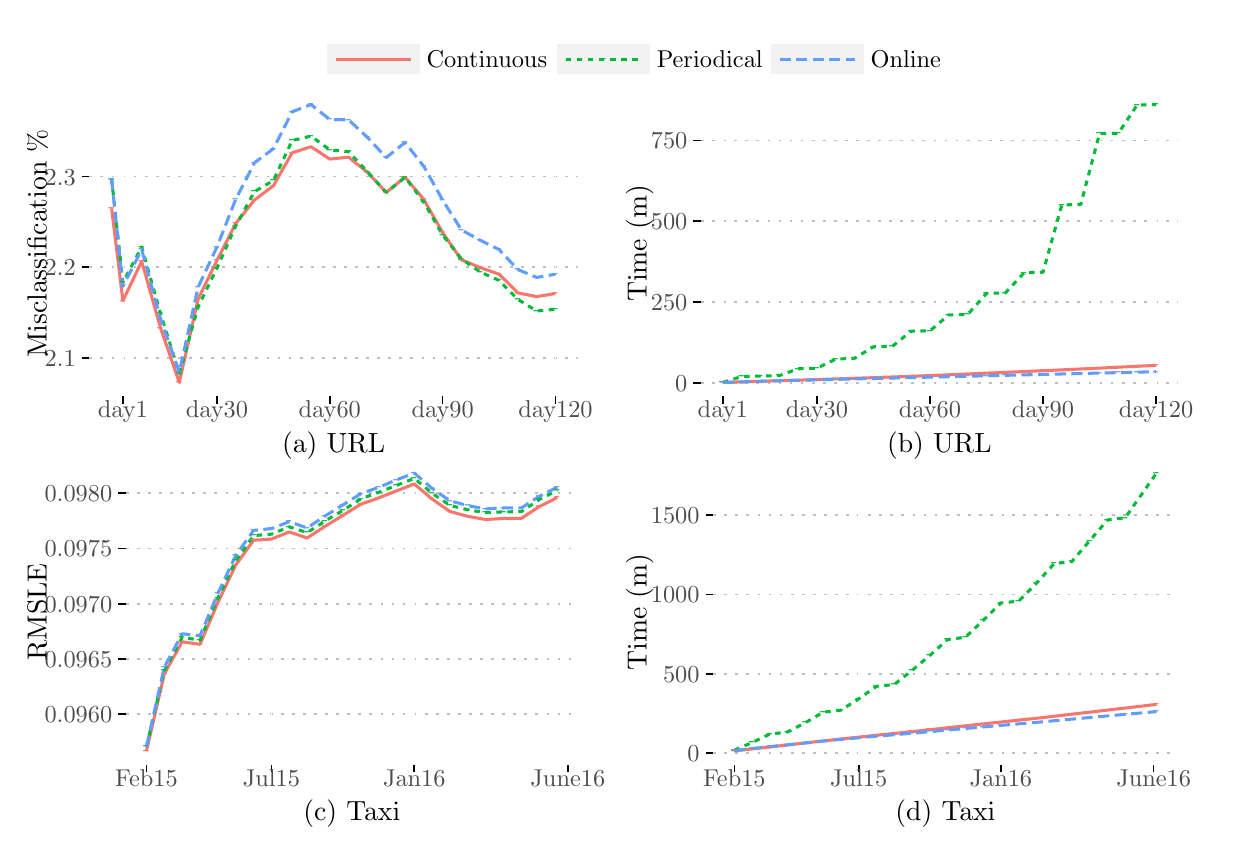
\begin{tikzpicture}[x=1pt,y=1pt]
\definecolor{fillColor}{RGB}{255,255,255}
\path[use as bounding box,fill=fillColor,fill opacity=0.00] (0,0) rectangle (433.62,289.08);
\begin{scope}
\path[clip] (  0.00,  0.00) rectangle (433.62,289.08);
\definecolor{fillColor}{RGB}{255,255,255}

\path[fill=fillColor] ( 97.81,266.32) rectangle (335.81,289.08);
\end{scope}
\begin{scope}
\path[clip] (  0.00,  0.00) rectangle (433.62,289.08);
\definecolor{drawColor}{RGB}{255,255,255}
\definecolor{fillColor}{gray}{0.95}

\path[draw=drawColor,line width= 0.6pt,line join=round,line cap=round,fill=fillColor] (107.84,272.01) rectangle (141.98,283.39);
\end{scope}
\begin{scope}
\path[clip] (  0.00,  0.00) rectangle (433.62,289.08);
\definecolor{drawColor}{RGB}{248,118,109}

\path[draw=drawColor,line width= 1.1pt,line join=round] (111.25,277.70) -- (138.57,277.70);
\end{scope}
\begin{scope}
\path[clip] (  0.00,  0.00) rectangle (433.62,289.08);
\definecolor{drawColor}{RGB}{248,118,109}

\node[text=drawColor,anchor=base,inner sep=0pt, outer sep=0pt, scale=  0.72] at (124.91,276.15) {-};
\end{scope}
\begin{scope}
\path[clip] (  0.00,  0.00) rectangle (433.62,289.08);
\definecolor{drawColor}{RGB}{255,255,255}
\definecolor{fillColor}{gray}{0.95}

\path[draw=drawColor,line width= 0.6pt,line join=round,line cap=round,fill=fillColor] (191.01,272.01) rectangle (225.15,283.39);
\end{scope}
\begin{scope}
\path[clip] (  0.00,  0.00) rectangle (433.62,289.08);
\definecolor{drawColor}{RGB}{0,186,56}

\path[draw=drawColor,line width= 1.1pt,dash pattern=on 2pt off 2pt ,line join=round] (194.42,277.70) -- (221.74,277.70);
\end{scope}
\begin{scope}
\path[clip] (  0.00,  0.00) rectangle (433.62,289.08);
\definecolor{drawColor}{RGB}{0,186,56}

\node[text=drawColor,anchor=base,inner sep=0pt, outer sep=0pt, scale=  0.72] at (208.08,276.15) {-};
\end{scope}
\begin{scope}
\path[clip] (  0.00,  0.00) rectangle (433.62,289.08);
\definecolor{drawColor}{RGB}{255,255,255}
\definecolor{fillColor}{gray}{0.95}

\path[draw=drawColor,line width= 0.6pt,line join=round,line cap=round,fill=fillColor] (268.27,272.01) rectangle (302.42,283.39);
\end{scope}
\begin{scope}
\path[clip] (  0.00,  0.00) rectangle (433.62,289.08);
\definecolor{drawColor}{RGB}{97,156,255}

\path[draw=drawColor,line width= 1.1pt,dash pattern=on 4pt off 2pt ,line join=round] (271.69,277.70) -- (299.00,277.70);
\end{scope}
\begin{scope}
\path[clip] (  0.00,  0.00) rectangle (433.62,289.08);
\definecolor{drawColor}{RGB}{97,156,255}

\node[text=drawColor,anchor=base,inner sep=0pt, outer sep=0pt, scale=  0.72] at (285.34,276.15) {-};
\end{scope}
\begin{scope}
\path[clip] (  0.00,  0.00) rectangle (433.62,289.08);
\definecolor{drawColor}{RGB}{0,0,0}

\node[text=drawColor,anchor=base west,inner sep=0pt, outer sep=0pt, scale=  0.88] at (144.15,274.67) {Continuous};
\end{scope}
\begin{scope}
\path[clip] (  0.00,  0.00) rectangle (433.62,289.08);
\definecolor{drawColor}{RGB}{0,0,0}

\node[text=drawColor,anchor=base west,inner sep=0pt, outer sep=0pt, scale=  0.88] at (227.32,274.67) {Periodical};
\end{scope}
\begin{scope}
\path[clip] (  0.00,  0.00) rectangle (433.62,289.08);
\definecolor{drawColor}{RGB}{0,0,0}

\node[text=drawColor,anchor=base west,inner sep=0pt, outer sep=0pt, scale=  0.88] at (304.58,274.67) {Online};
\end{scope}
\begin{scope}
\path[clip] (  0.00,133.16) rectangle (216.81,266.32);
\definecolor{drawColor}{RGB}{255,255,255}
\definecolor{fillColor}{RGB}{255,255,255}

\path[draw=drawColor,line width= 0.6pt,line join=round,line cap=round,fill=fillColor] (  0.00,133.16) rectangle (216.81,266.32);
\end{scope}
\begin{scope}
\path[clip] ( 22.31,155.85) rectangle (198.74,266.32);
\definecolor{fillColor}{RGB}{255,255,255}

\path[fill=fillColor] ( 22.31,155.85) rectangle (198.74,266.32);
\definecolor{drawColor}{RGB}{255,255,255}

\path[draw=drawColor,line width= 0.3pt,line join=round] ( 22.31,186.15) --
	(198.74,186.15);

\path[draw=drawColor,line width= 0.3pt,line join=round] ( 22.31,218.88) --
	(198.74,218.88);

\path[draw=drawColor,line width= 0.3pt,line join=round] ( 22.31,251.60) --
	(198.74,251.60);

\path[draw=drawColor,line width= 0.3pt,line join=round] ( 51.40,155.85) --
	( 51.40,266.32);

\path[draw=drawColor,line width= 0.3pt,line join=round] ( 88.78,155.85) --
	( 88.78,266.32);

\path[draw=drawColor,line width= 0.3pt,line join=round] (129.56,155.85) --
	(129.56,266.32);

\path[draw=drawColor,line width= 0.3pt,line join=round] (170.33,155.85) --
	(170.33,266.32);
\definecolor{drawColor}{RGB}{190,190,190}

\path[draw=drawColor,line width= 0.6pt,dash pattern=on 1pt off 3pt ,line join=round] ( 22.31,169.79) --
	(198.74,169.79);

\path[draw=drawColor,line width= 0.6pt,dash pattern=on 1pt off 3pt ,line join=round] ( 22.31,202.51) --
	(198.74,202.51);

\path[draw=drawColor,line width= 0.6pt,dash pattern=on 1pt off 3pt ,line join=round] ( 22.31,235.24) --
	(198.74,235.24);
\definecolor{drawColor}{RGB}{255,255,255}

\path[draw=drawColor,line width= 0.6pt,line join=round] ( 34.41,155.85) --
	( 34.41,266.32);

\path[draw=drawColor,line width= 0.6pt,line join=round] ( 68.39,155.85) --
	( 68.39,266.32);

\path[draw=drawColor,line width= 0.6pt,line join=round] (109.17,155.85) --
	(109.17,266.32);

\path[draw=drawColor,line width= 0.6pt,line join=round] (149.94,155.85) --
	(149.94,266.32);

\path[draw=drawColor,line width= 0.6pt,line join=round] (190.72,155.85) --
	(190.72,266.32);
\definecolor{drawColor}{RGB}{248,118,109}

\path[draw=drawColor,line width= 1.1pt,line join=round] ( 30.33,223.79) --
	( 34.41,190.41) --
	( 41.20,204.64) --
	( 48.00,180.59) --
	( 54.79,160.87) --
	( 61.59,191.06) --
	( 68.39,204.97) --
	( 75.18,218.32) --
	( 81.98,226.85) --
	( 88.78,231.93) --
	( 95.57,243.85) --
	(102.37,246.06) --
	(109.17,241.59) --
	(115.96,242.27) --
	(122.76,236.85) --
	(129.56,229.54) --
	(136.35,235.07) --
	(143.15,226.98) --
	(149.94,215.02) --
	(156.74,205.20) --
	(163.54,202.38) --
	(170.33,200.00) --
	(177.13,193.24) --
	(183.93,191.90) --
	(190.72,193.00);
\definecolor{drawColor}{RGB}{0,186,56}

\path[draw=drawColor,line width= 1.1pt,dash pattern=on 2pt off 2pt ,line join=round] ( 30.33,234.42) --
	( 34.41,196.95) --
	( 41.20,209.88) --
	( 48.00,185.82) --
	( 54.79,164.14) --
	( 61.59,188.18) --
	( 68.39,202.19) --
	( 75.18,217.48) --
	( 81.98,229.88) --
	( 88.78,233.81) --
	( 95.57,248.30) --
	(102.37,249.91) --
	(109.17,244.92) --
	(115.96,244.26) --
	(122.76,237.00) --
	(129.56,229.51) --
	(136.35,234.99) --
	(143.15,226.07) --
	(149.94,214.14) --
	(156.74,205.49) --
	(163.54,200.81) --
	(170.33,197.75) --
	(177.13,190.88) --
	(183.93,186.71) --
	(190.72,187.32);
\definecolor{drawColor}{RGB}{97,156,255}

\path[draw=drawColor,line width= 1.1pt,dash pattern=on 4pt off 2pt ,line join=round] ( 30.33,234.42) --
	( 34.41,195.64) --
	( 41.20,208.90) --
	( 48.00,183.86) --
	( 54.79,164.63) --
	( 61.59,195.32) --
	( 68.39,209.82) --
	( 75.18,227.06) --
	( 81.98,240.27) --
	( 88.78,245.32) --
	( 95.57,258.68) --
	(102.37,261.30) --
	(109.17,255.90) --
	(115.96,255.77) --
	(122.76,249.47) --
	(129.56,242.12) --
	(136.35,247.58) --
	(143.15,238.96) --
	(149.94,226.77) --
	(156.74,215.99) --
	(163.54,212.25) --
	(170.33,208.90) --
	(177.13,201.68) --
	(183.93,198.83) --
	(190.72,200.00);
\definecolor{drawColor}{RGB}{248,118,109}

\node[text=drawColor,anchor=base,inner sep=0pt, outer sep=0pt, scale=  0.72] at ( 30.33,222.24) {-};

\node[text=drawColor,anchor=base,inner sep=0pt, outer sep=0pt, scale=  0.72] at ( 34.41,188.86) {-};

\node[text=drawColor,anchor=base,inner sep=0pt, outer sep=0pt, scale=  0.72] at ( 41.20,203.09) {-};

\node[text=drawColor,anchor=base,inner sep=0pt, outer sep=0pt, scale=  0.72] at ( 48.00,179.04) {-};

\node[text=drawColor,anchor=base,inner sep=0pt, outer sep=0pt, scale=  0.72] at ( 54.79,159.32) {-};

\node[text=drawColor,anchor=base,inner sep=0pt, outer sep=0pt, scale=  0.72] at ( 61.59,189.51) {-};

\node[text=drawColor,anchor=base,inner sep=0pt, outer sep=0pt, scale=  0.72] at ( 68.39,203.42) {-};

\node[text=drawColor,anchor=base,inner sep=0pt, outer sep=0pt, scale=  0.72] at ( 75.18,216.77) {-};

\node[text=drawColor,anchor=base,inner sep=0pt, outer sep=0pt, scale=  0.72] at ( 81.98,225.30) {-};

\node[text=drawColor,anchor=base,inner sep=0pt, outer sep=0pt, scale=  0.72] at ( 88.78,230.38) {-};

\node[text=drawColor,anchor=base,inner sep=0pt, outer sep=0pt, scale=  0.72] at ( 95.57,242.30) {-};

\node[text=drawColor,anchor=base,inner sep=0pt, outer sep=0pt, scale=  0.72] at (102.37,244.51) {-};

\node[text=drawColor,anchor=base,inner sep=0pt, outer sep=0pt, scale=  0.72] at (109.17,240.04) {-};

\node[text=drawColor,anchor=base,inner sep=0pt, outer sep=0pt, scale=  0.72] at (115.96,240.72) {-};

\node[text=drawColor,anchor=base,inner sep=0pt, outer sep=0pt, scale=  0.72] at (122.76,235.30) {-};

\node[text=drawColor,anchor=base,inner sep=0pt, outer sep=0pt, scale=  0.72] at (129.56,227.99) {-};

\node[text=drawColor,anchor=base,inner sep=0pt, outer sep=0pt, scale=  0.72] at (136.35,233.52) {-};

\node[text=drawColor,anchor=base,inner sep=0pt, outer sep=0pt, scale=  0.72] at (143.15,225.43) {-};

\node[text=drawColor,anchor=base,inner sep=0pt, outer sep=0pt, scale=  0.72] at (149.94,213.47) {-};

\node[text=drawColor,anchor=base,inner sep=0pt, outer sep=0pt, scale=  0.72] at (156.74,203.65) {-};

\node[text=drawColor,anchor=base,inner sep=0pt, outer sep=0pt, scale=  0.72] at (163.54,200.83) {-};

\node[text=drawColor,anchor=base,inner sep=0pt, outer sep=0pt, scale=  0.72] at (170.33,198.45) {-};

\node[text=drawColor,anchor=base,inner sep=0pt, outer sep=0pt, scale=  0.72] at (177.13,191.69) {-};

\node[text=drawColor,anchor=base,inner sep=0pt, outer sep=0pt, scale=  0.72] at (183.93,190.35) {-};

\node[text=drawColor,anchor=base,inner sep=0pt, outer sep=0pt, scale=  0.72] at (190.72,191.45) {-};
\definecolor{drawColor}{RGB}{0,186,56}

\node[text=drawColor,anchor=base,inner sep=0pt, outer sep=0pt, scale=  0.72] at ( 30.33,232.87) {-};

\node[text=drawColor,anchor=base,inner sep=0pt, outer sep=0pt, scale=  0.72] at ( 34.41,195.40) {-};

\node[text=drawColor,anchor=base,inner sep=0pt, outer sep=0pt, scale=  0.72] at ( 41.20,208.33) {-};

\node[text=drawColor,anchor=base,inner sep=0pt, outer sep=0pt, scale=  0.72] at ( 48.00,184.27) {-};

\node[text=drawColor,anchor=base,inner sep=0pt, outer sep=0pt, scale=  0.72] at ( 54.79,162.59) {-};

\node[text=drawColor,anchor=base,inner sep=0pt, outer sep=0pt, scale=  0.72] at ( 61.59,186.63) {-};

\node[text=drawColor,anchor=base,inner sep=0pt, outer sep=0pt, scale=  0.72] at ( 68.39,200.64) {-};

\node[text=drawColor,anchor=base,inner sep=0pt, outer sep=0pt, scale=  0.72] at ( 75.18,215.92) {-};

\node[text=drawColor,anchor=base,inner sep=0pt, outer sep=0pt, scale=  0.72] at ( 81.98,228.33) {-};

\node[text=drawColor,anchor=base,inner sep=0pt, outer sep=0pt, scale=  0.72] at ( 88.78,232.26) {-};

\node[text=drawColor,anchor=base,inner sep=0pt, outer sep=0pt, scale=  0.72] at ( 95.57,246.74) {-};

\node[text=drawColor,anchor=base,inner sep=0pt, outer sep=0pt, scale=  0.72] at (102.37,248.35) {-};

\node[text=drawColor,anchor=base,inner sep=0pt, outer sep=0pt, scale=  0.72] at (109.17,243.37) {-};

\node[text=drawColor,anchor=base,inner sep=0pt, outer sep=0pt, scale=  0.72] at (115.96,242.71) {-};

\node[text=drawColor,anchor=base,inner sep=0pt, outer sep=0pt, scale=  0.72] at (122.76,235.44) {-};

\node[text=drawColor,anchor=base,inner sep=0pt, outer sep=0pt, scale=  0.72] at (129.56,227.96) {-};

\node[text=drawColor,anchor=base,inner sep=0pt, outer sep=0pt, scale=  0.72] at (136.35,233.44) {-};

\node[text=drawColor,anchor=base,inner sep=0pt, outer sep=0pt, scale=  0.72] at (143.15,224.52) {-};

\node[text=drawColor,anchor=base,inner sep=0pt, outer sep=0pt, scale=  0.72] at (149.94,212.59) {-};

\node[text=drawColor,anchor=base,inner sep=0pt, outer sep=0pt, scale=  0.72] at (156.74,203.94) {-};

\node[text=drawColor,anchor=base,inner sep=0pt, outer sep=0pt, scale=  0.72] at (163.54,199.26) {-};

\node[text=drawColor,anchor=base,inner sep=0pt, outer sep=0pt, scale=  0.72] at (170.33,196.20) {-};

\node[text=drawColor,anchor=base,inner sep=0pt, outer sep=0pt, scale=  0.72] at (177.13,189.33) {-};

\node[text=drawColor,anchor=base,inner sep=0pt, outer sep=0pt, scale=  0.72] at (183.93,185.16) {-};

\node[text=drawColor,anchor=base,inner sep=0pt, outer sep=0pt, scale=  0.72] at (190.72,185.77) {-};
\definecolor{drawColor}{RGB}{97,156,255}

\node[text=drawColor,anchor=base,inner sep=0pt, outer sep=0pt, scale=  0.72] at ( 30.33,232.87) {-};

\node[text=drawColor,anchor=base,inner sep=0pt, outer sep=0pt, scale=  0.72] at ( 34.41,194.09) {-};

\node[text=drawColor,anchor=base,inner sep=0pt, outer sep=0pt, scale=  0.72] at ( 41.20,207.35) {-};

\node[text=drawColor,anchor=base,inner sep=0pt, outer sep=0pt, scale=  0.72] at ( 48.00,182.31) {-};

\node[text=drawColor,anchor=base,inner sep=0pt, outer sep=0pt, scale=  0.72] at ( 54.79,163.08) {-};

\node[text=drawColor,anchor=base,inner sep=0pt, outer sep=0pt, scale=  0.72] at ( 61.59,193.76) {-};

\node[text=drawColor,anchor=base,inner sep=0pt, outer sep=0pt, scale=  0.72] at ( 68.39,208.27) {-};

\node[text=drawColor,anchor=base,inner sep=0pt, outer sep=0pt, scale=  0.72] at ( 75.18,225.51) {-};

\node[text=drawColor,anchor=base,inner sep=0pt, outer sep=0pt, scale=  0.72] at ( 81.98,238.72) {-};

\node[text=drawColor,anchor=base,inner sep=0pt, outer sep=0pt, scale=  0.72] at ( 88.78,243.77) {-};

\node[text=drawColor,anchor=base,inner sep=0pt, outer sep=0pt, scale=  0.72] at ( 95.57,257.13) {-};

\node[text=drawColor,anchor=base,inner sep=0pt, outer sep=0pt, scale=  0.72] at (102.37,259.75) {-};

\node[text=drawColor,anchor=base,inner sep=0pt, outer sep=0pt, scale=  0.72] at (109.17,254.35) {-};

\node[text=drawColor,anchor=base,inner sep=0pt, outer sep=0pt, scale=  0.72] at (115.96,254.22) {-};

\node[text=drawColor,anchor=base,inner sep=0pt, outer sep=0pt, scale=  0.72] at (122.76,247.92) {-};

\node[text=drawColor,anchor=base,inner sep=0pt, outer sep=0pt, scale=  0.72] at (129.56,240.57) {-};

\node[text=drawColor,anchor=base,inner sep=0pt, outer sep=0pt, scale=  0.72] at (136.35,246.03) {-};

\node[text=drawColor,anchor=base,inner sep=0pt, outer sep=0pt, scale=  0.72] at (143.15,237.41) {-};

\node[text=drawColor,anchor=base,inner sep=0pt, outer sep=0pt, scale=  0.72] at (149.94,225.22) {-};

\node[text=drawColor,anchor=base,inner sep=0pt, outer sep=0pt, scale=  0.72] at (156.74,214.44) {-};

\node[text=drawColor,anchor=base,inner sep=0pt, outer sep=0pt, scale=  0.72] at (163.54,210.70) {-};

\node[text=drawColor,anchor=base,inner sep=0pt, outer sep=0pt, scale=  0.72] at (170.33,207.35) {-};

\node[text=drawColor,anchor=base,inner sep=0pt, outer sep=0pt, scale=  0.72] at (177.13,200.13) {-};

\node[text=drawColor,anchor=base,inner sep=0pt, outer sep=0pt, scale=  0.72] at (183.93,197.28) {-};

\node[text=drawColor,anchor=base,inner sep=0pt, outer sep=0pt, scale=  0.72] at (190.72,198.45) {-};
\end{scope}
\begin{scope}
\path[clip] (  0.00,  0.00) rectangle (433.62,289.08);
\definecolor{drawColor}{gray}{0.30}

\node[text=drawColor,anchor=base east,inner sep=0pt, outer sep=0pt, scale=  0.88] at ( 17.36,166.76) {2.1};

\node[text=drawColor,anchor=base east,inner sep=0pt, outer sep=0pt, scale=  0.88] at ( 17.36,199.48) {2.2};

\node[text=drawColor,anchor=base east,inner sep=0pt, outer sep=0pt, scale=  0.88] at ( 17.36,232.21) {2.3};
\end{scope}
\begin{scope}
\path[clip] (  0.00,  0.00) rectangle (433.62,289.08);
\definecolor{drawColor}{RGB}{0,0,0}

\path[draw=drawColor,line width= 0.6pt,line join=round] ( 19.56,169.79) --
	( 22.31,169.79);

\path[draw=drawColor,line width= 0.6pt,line join=round] ( 19.56,202.51) --
	( 22.31,202.51);

\path[draw=drawColor,line width= 0.6pt,line join=round] ( 19.56,235.24) --
	( 22.31,235.24);
\end{scope}
\begin{scope}
\path[clip] (  0.00,  0.00) rectangle (433.62,289.08);
\definecolor{drawColor}{RGB}{0,0,0}

\path[draw=drawColor,line width= 0.6pt,line join=round] ( 34.41,153.10) --
	( 34.41,155.85);

\path[draw=drawColor,line width= 0.6pt,line join=round] ( 68.39,153.10) --
	( 68.39,155.85);

\path[draw=drawColor,line width= 0.6pt,line join=round] (109.17,153.10) --
	(109.17,155.85);

\path[draw=drawColor,line width= 0.6pt,line join=round] (149.94,153.10) --
	(149.94,155.85);

\path[draw=drawColor,line width= 0.6pt,line join=round] (190.72,153.10) --
	(190.72,155.85);
\end{scope}
\begin{scope}
\path[clip] (  0.00,  0.00) rectangle (433.62,289.08);
\definecolor{drawColor}{gray}{0.30}

\node[text=drawColor,anchor=base,inner sep=0pt, outer sep=0pt, scale=  0.88] at ( 34.41,148.04) {day1};

\node[text=drawColor,anchor=base,inner sep=0pt, outer sep=0pt, scale=  0.88] at ( 68.39,148.04) {day30};

\node[text=drawColor,anchor=base,inner sep=0pt, outer sep=0pt, scale=  0.88] at (109.17,148.04) {day60};

\node[text=drawColor,anchor=base,inner sep=0pt, outer sep=0pt, scale=  0.88] at (149.94,148.04) {day90};

\node[text=drawColor,anchor=base,inner sep=0pt, outer sep=0pt, scale=  0.88] at (190.72,148.04) {day120};
\end{scope}
\begin{scope}
\path[clip] (  0.00,  0.00) rectangle (433.62,289.08);
\definecolor{drawColor}{RGB}{0,0,0}

\node[text=drawColor,anchor=base,inner sep=0pt, outer sep=0pt, scale=  1.00] at (110.53,135.65) {(a) URL};
\end{scope}
\begin{scope}
\path[clip] (  0.00,  0.00) rectangle (433.62,289.08);
\definecolor{drawColor}{RGB}{0,0,0}

\node[text=drawColor,rotate= 90.00,anchor=base,inner sep=0pt, outer sep=0pt, scale=  1.00] at (  6.89,211.08) {Misclassification \%};
\end{scope}
\begin{scope}
\path[clip] (216.81,133.16) rectangle (433.62,266.32);
\definecolor{drawColor}{RGB}{255,255,255}
\definecolor{fillColor}{RGB}{255,255,255}

\path[draw=drawColor,line width= 0.6pt,line join=round,line cap=round,fill=fillColor] (216.81,133.16) rectangle (433.62,266.32);
\end{scope}
\begin{scope}
\path[clip] (243.34,155.85) rectangle (415.55,266.32);
\definecolor{fillColor}{RGB}{255,255,255}

\path[fill=fillColor] (243.34,155.85) rectangle (415.55,266.32);
\definecolor{drawColor}{RGB}{255,255,255}

\path[draw=drawColor,line width= 0.3pt,line join=round] (243.34,175.29) --
	(415.55,175.29);

\path[draw=drawColor,line width= 0.3pt,line join=round] (243.34,204.50) --
	(415.55,204.50);

\path[draw=drawColor,line width= 0.3pt,line join=round] (243.34,233.72) --
	(415.55,233.72);

\path[draw=drawColor,line width= 0.3pt,line join=round] (243.34,262.93) --
	(415.55,262.93);

\path[draw=drawColor,line width= 0.3pt,line join=round] (268.18,155.85) --
	(268.18,266.32);

\path[draw=drawColor,line width= 0.3pt,line join=round] (305.62,155.85) --
	(305.62,266.32);

\path[draw=drawColor,line width= 0.3pt,line join=round] (346.46,155.85) --
	(346.46,266.32);

\path[draw=drawColor,line width= 0.3pt,line join=round] (387.30,155.85) --
	(387.30,266.32);
\definecolor{drawColor}{RGB}{190,190,190}

\path[draw=drawColor,line width= 0.6pt,dash pattern=on 1pt off 3pt ,line join=round] (243.34,160.69) --
	(415.55,160.69);

\path[draw=drawColor,line width= 0.6pt,dash pattern=on 1pt off 3pt ,line join=round] (243.34,189.90) --
	(415.55,189.90);

\path[draw=drawColor,line width= 0.6pt,dash pattern=on 1pt off 3pt ,line join=round] (243.34,219.11) --
	(415.55,219.11);

\path[draw=drawColor,line width= 0.6pt,dash pattern=on 1pt off 3pt ,line join=round] (243.34,248.32) --
	(415.55,248.32);
\definecolor{drawColor}{RGB}{255,255,255}

\path[draw=drawColor,line width= 0.6pt,line join=round] (251.17,155.85) --
	(251.17,266.32);

\path[draw=drawColor,line width= 0.6pt,line join=round] (285.20,155.85) --
	(285.20,266.32);

\path[draw=drawColor,line width= 0.6pt,line join=round] (326.04,155.85) --
	(326.04,266.32);

\path[draw=drawColor,line width= 0.6pt,line join=round] (366.88,155.85) --
	(366.88,266.32);

\path[draw=drawColor,line width= 0.6pt,line join=round] (407.72,155.85) --
	(407.72,266.32);
\definecolor{drawColor}{RGB}{248,118,109}

\path[draw=drawColor,line width= 1.1pt,line join=round] (251.17,160.89) --
	(257.97,161.09) --
	(264.78,161.30) --
	(271.59,161.50) --
	(278.39,161.71) --
	(285.20,161.92) --
	(292.01,162.16) --
	(298.81,162.39) --
	(305.62,162.61) --
	(312.43,162.86) --
	(319.23,163.10) --
	(326.04,163.37) --
	(332.85,163.65) --
	(339.66,163.95) --
	(346.46,164.24) --
	(353.27,164.53) --
	(360.08,164.82) --
	(366.88,165.13) --
	(373.69,165.43) --
	(380.50,165.75) --
	(387.30,166.06) --
	(394.11,166.39) --
	(400.92,166.72) --
	(407.72,167.07);
\definecolor{drawColor}{RGB}{0,186,56}

\path[draw=drawColor,line width= 1.1pt,dash pattern=on 2pt off 2pt ,line join=round] (251.17,160.90) --
	(257.97,163.01) --
	(264.78,163.18) --
	(271.59,163.35) --
	(278.39,165.82) --
	(285.20,166.03) --
	(292.01,169.31) --
	(298.81,169.62) --
	(305.62,173.77) --
	(312.43,173.93) --
	(319.23,179.39) --
	(326.04,179.54) --
	(332.85,185.30) --
	(339.66,185.45) --
	(346.46,193.05) --
	(353.27,193.23) --
	(360.08,200.53) --
	(366.88,200.71) --
	(373.69,225.03) --
	(380.50,225.17) --
	(387.30,250.78) --
	(394.11,250.93) --
	(400.92,261.15) --
	(407.72,261.30);
\definecolor{drawColor}{RGB}{97,156,255}

\path[draw=drawColor,line width= 1.1pt,dash pattern=on 4pt off 2pt ,line join=round] (251.17,160.87) --
	(257.97,161.04) --
	(264.78,161.32) --
	(271.59,161.49) --
	(278.39,161.66) --
	(285.20,161.82) --
	(292.01,161.99) --
	(298.81,162.16) --
	(305.62,162.30) --
	(312.43,162.47) --
	(319.23,162.63) --
	(326.04,162.80) --
	(332.85,162.96) --
	(339.66,163.13) --
	(346.46,163.29) --
	(353.27,163.45) --
	(360.08,163.62) --
	(366.88,163.78) --
	(373.69,163.94) --
	(380.50,164.11) --
	(387.30,164.27) --
	(394.11,164.43) --
	(400.92,164.60) --
	(407.72,164.76);
\definecolor{drawColor}{RGB}{248,118,109}

\node[text=drawColor,anchor=base,inner sep=0pt, outer sep=0pt, scale=  0.72] at (251.17,159.34) {-};

\node[text=drawColor,anchor=base,inner sep=0pt, outer sep=0pt, scale=  0.72] at (257.97,159.54) {-};

\node[text=drawColor,anchor=base,inner sep=0pt, outer sep=0pt, scale=  0.72] at (264.78,159.75) {-};

\node[text=drawColor,anchor=base,inner sep=0pt, outer sep=0pt, scale=  0.72] at (271.59,159.95) {-};

\node[text=drawColor,anchor=base,inner sep=0pt, outer sep=0pt, scale=  0.72] at (278.39,160.16) {-};

\node[text=drawColor,anchor=base,inner sep=0pt, outer sep=0pt, scale=  0.72] at (285.20,160.37) {-};

\node[text=drawColor,anchor=base,inner sep=0pt, outer sep=0pt, scale=  0.72] at (292.01,160.61) {-};

\node[text=drawColor,anchor=base,inner sep=0pt, outer sep=0pt, scale=  0.72] at (298.81,160.84) {-};

\node[text=drawColor,anchor=base,inner sep=0pt, outer sep=0pt, scale=  0.72] at (305.62,161.06) {-};

\node[text=drawColor,anchor=base,inner sep=0pt, outer sep=0pt, scale=  0.72] at (312.43,161.31) {-};

\node[text=drawColor,anchor=base,inner sep=0pt, outer sep=0pt, scale=  0.72] at (319.23,161.55) {-};

\node[text=drawColor,anchor=base,inner sep=0pt, outer sep=0pt, scale=  0.72] at (326.04,161.82) {-};

\node[text=drawColor,anchor=base,inner sep=0pt, outer sep=0pt, scale=  0.72] at (332.85,162.10) {-};

\node[text=drawColor,anchor=base,inner sep=0pt, outer sep=0pt, scale=  0.72] at (339.66,162.40) {-};

\node[text=drawColor,anchor=base,inner sep=0pt, outer sep=0pt, scale=  0.72] at (346.46,162.69) {-};

\node[text=drawColor,anchor=base,inner sep=0pt, outer sep=0pt, scale=  0.72] at (353.27,162.98) {-};

\node[text=drawColor,anchor=base,inner sep=0pt, outer sep=0pt, scale=  0.72] at (360.08,163.27) {-};

\node[text=drawColor,anchor=base,inner sep=0pt, outer sep=0pt, scale=  0.72] at (366.88,163.58) {-};

\node[text=drawColor,anchor=base,inner sep=0pt, outer sep=0pt, scale=  0.72] at (373.69,163.88) {-};

\node[text=drawColor,anchor=base,inner sep=0pt, outer sep=0pt, scale=  0.72] at (380.50,164.19) {-};

\node[text=drawColor,anchor=base,inner sep=0pt, outer sep=0pt, scale=  0.72] at (387.30,164.51) {-};

\node[text=drawColor,anchor=base,inner sep=0pt, outer sep=0pt, scale=  0.72] at (394.11,164.84) {-};

\node[text=drawColor,anchor=base,inner sep=0pt, outer sep=0pt, scale=  0.72] at (400.92,165.17) {-};

\node[text=drawColor,anchor=base,inner sep=0pt, outer sep=0pt, scale=  0.72] at (407.72,165.52) {-};
\definecolor{drawColor}{RGB}{0,186,56}

\node[text=drawColor,anchor=base,inner sep=0pt, outer sep=0pt, scale=  0.72] at (251.17,159.35) {-};

\node[text=drawColor,anchor=base,inner sep=0pt, outer sep=0pt, scale=  0.72] at (257.97,161.46) {-};

\node[text=drawColor,anchor=base,inner sep=0pt, outer sep=0pt, scale=  0.72] at (264.78,161.63) {-};

\node[text=drawColor,anchor=base,inner sep=0pt, outer sep=0pt, scale=  0.72] at (271.59,161.80) {-};

\node[text=drawColor,anchor=base,inner sep=0pt, outer sep=0pt, scale=  0.72] at (278.39,164.27) {-};

\node[text=drawColor,anchor=base,inner sep=0pt, outer sep=0pt, scale=  0.72] at (285.20,164.47) {-};

\node[text=drawColor,anchor=base,inner sep=0pt, outer sep=0pt, scale=  0.72] at (292.01,167.76) {-};

\node[text=drawColor,anchor=base,inner sep=0pt, outer sep=0pt, scale=  0.72] at (298.81,168.07) {-};

\node[text=drawColor,anchor=base,inner sep=0pt, outer sep=0pt, scale=  0.72] at (305.62,172.22) {-};

\node[text=drawColor,anchor=base,inner sep=0pt, outer sep=0pt, scale=  0.72] at (312.43,172.38) {-};

\node[text=drawColor,anchor=base,inner sep=0pt, outer sep=0pt, scale=  0.72] at (319.23,177.83) {-};

\node[text=drawColor,anchor=base,inner sep=0pt, outer sep=0pt, scale=  0.72] at (326.04,177.99) {-};

\node[text=drawColor,anchor=base,inner sep=0pt, outer sep=0pt, scale=  0.72] at (332.85,183.75) {-};

\node[text=drawColor,anchor=base,inner sep=0pt, outer sep=0pt, scale=  0.72] at (339.66,183.90) {-};

\node[text=drawColor,anchor=base,inner sep=0pt, outer sep=0pt, scale=  0.72] at (346.46,191.50) {-};

\node[text=drawColor,anchor=base,inner sep=0pt, outer sep=0pt, scale=  0.72] at (353.27,191.68) {-};

\node[text=drawColor,anchor=base,inner sep=0pt, outer sep=0pt, scale=  0.72] at (360.08,198.98) {-};

\node[text=drawColor,anchor=base,inner sep=0pt, outer sep=0pt, scale=  0.72] at (366.88,199.16) {-};

\node[text=drawColor,anchor=base,inner sep=0pt, outer sep=0pt, scale=  0.72] at (373.69,223.48) {-};

\node[text=drawColor,anchor=base,inner sep=0pt, outer sep=0pt, scale=  0.72] at (380.50,223.62) {-};

\node[text=drawColor,anchor=base,inner sep=0pt, outer sep=0pt, scale=  0.72] at (387.30,249.23) {-};

\node[text=drawColor,anchor=base,inner sep=0pt, outer sep=0pt, scale=  0.72] at (394.11,249.38) {-};

\node[text=drawColor,anchor=base,inner sep=0pt, outer sep=0pt, scale=  0.72] at (400.92,259.60) {-};

\node[text=drawColor,anchor=base,inner sep=0pt, outer sep=0pt, scale=  0.72] at (407.72,259.75) {-};
\definecolor{drawColor}{RGB}{97,156,255}

\node[text=drawColor,anchor=base,inner sep=0pt, outer sep=0pt, scale=  0.72] at (251.17,159.32) {-};

\node[text=drawColor,anchor=base,inner sep=0pt, outer sep=0pt, scale=  0.72] at (257.97,159.49) {-};

\node[text=drawColor,anchor=base,inner sep=0pt, outer sep=0pt, scale=  0.72] at (264.78,159.77) {-};

\node[text=drawColor,anchor=base,inner sep=0pt, outer sep=0pt, scale=  0.72] at (271.59,159.94) {-};

\node[text=drawColor,anchor=base,inner sep=0pt, outer sep=0pt, scale=  0.72] at (278.39,160.11) {-};

\node[text=drawColor,anchor=base,inner sep=0pt, outer sep=0pt, scale=  0.72] at (285.20,160.27) {-};

\node[text=drawColor,anchor=base,inner sep=0pt, outer sep=0pt, scale=  0.72] at (292.01,160.44) {-};

\node[text=drawColor,anchor=base,inner sep=0pt, outer sep=0pt, scale=  0.72] at (298.81,160.61) {-};

\node[text=drawColor,anchor=base,inner sep=0pt, outer sep=0pt, scale=  0.72] at (305.62,160.75) {-};

\node[text=drawColor,anchor=base,inner sep=0pt, outer sep=0pt, scale=  0.72] at (312.43,160.92) {-};

\node[text=drawColor,anchor=base,inner sep=0pt, outer sep=0pt, scale=  0.72] at (319.23,161.08) {-};

\node[text=drawColor,anchor=base,inner sep=0pt, outer sep=0pt, scale=  0.72] at (326.04,161.25) {-};

\node[text=drawColor,anchor=base,inner sep=0pt, outer sep=0pt, scale=  0.72] at (332.85,161.41) {-};

\node[text=drawColor,anchor=base,inner sep=0pt, outer sep=0pt, scale=  0.72] at (339.66,161.58) {-};

\node[text=drawColor,anchor=base,inner sep=0pt, outer sep=0pt, scale=  0.72] at (346.46,161.74) {-};

\node[text=drawColor,anchor=base,inner sep=0pt, outer sep=0pt, scale=  0.72] at (353.27,161.90) {-};

\node[text=drawColor,anchor=base,inner sep=0pt, outer sep=0pt, scale=  0.72] at (360.08,162.07) {-};

\node[text=drawColor,anchor=base,inner sep=0pt, outer sep=0pt, scale=  0.72] at (366.88,162.23) {-};

\node[text=drawColor,anchor=base,inner sep=0pt, outer sep=0pt, scale=  0.72] at (373.69,162.39) {-};

\node[text=drawColor,anchor=base,inner sep=0pt, outer sep=0pt, scale=  0.72] at (380.50,162.56) {-};

\node[text=drawColor,anchor=base,inner sep=0pt, outer sep=0pt, scale=  0.72] at (387.30,162.72) {-};

\node[text=drawColor,anchor=base,inner sep=0pt, outer sep=0pt, scale=  0.72] at (394.11,162.88) {-};

\node[text=drawColor,anchor=base,inner sep=0pt, outer sep=0pt, scale=  0.72] at (400.92,163.05) {-};

\node[text=drawColor,anchor=base,inner sep=0pt, outer sep=0pt, scale=  0.72] at (407.72,163.21) {-};
\end{scope}
\begin{scope}
\path[clip] (  0.00,  0.00) rectangle (433.62,289.08);
\definecolor{drawColor}{gray}{0.30}

\node[text=drawColor,anchor=base east,inner sep=0pt, outer sep=0pt, scale=  0.88] at (238.39,157.66) {0};

\node[text=drawColor,anchor=base east,inner sep=0pt, outer sep=0pt, scale=  0.88] at (238.39,186.87) {250};

\node[text=drawColor,anchor=base east,inner sep=0pt, outer sep=0pt, scale=  0.88] at (238.39,216.08) {500};

\node[text=drawColor,anchor=base east,inner sep=0pt, outer sep=0pt, scale=  0.88] at (238.39,245.29) {750};
\end{scope}
\begin{scope}
\path[clip] (  0.00,  0.00) rectangle (433.62,289.08);
\definecolor{drawColor}{RGB}{0,0,0}

\path[draw=drawColor,line width= 0.6pt,line join=round] (240.59,160.69) --
	(243.34,160.69);

\path[draw=drawColor,line width= 0.6pt,line join=round] (240.59,189.90) --
	(243.34,189.90);

\path[draw=drawColor,line width= 0.6pt,line join=round] (240.59,219.11) --
	(243.34,219.11);

\path[draw=drawColor,line width= 0.6pt,line join=round] (240.59,248.32) --
	(243.34,248.32);
\end{scope}
\begin{scope}
\path[clip] (  0.00,  0.00) rectangle (433.62,289.08);
\definecolor{drawColor}{RGB}{0,0,0}

\path[draw=drawColor,line width= 0.6pt,line join=round] (251.17,153.10) --
	(251.17,155.85);

\path[draw=drawColor,line width= 0.6pt,line join=round] (285.20,153.10) --
	(285.20,155.85);

\path[draw=drawColor,line width= 0.6pt,line join=round] (326.04,153.10) --
	(326.04,155.85);

\path[draw=drawColor,line width= 0.6pt,line join=round] (366.88,153.10) --
	(366.88,155.85);

\path[draw=drawColor,line width= 0.6pt,line join=round] (407.72,153.10) --
	(407.72,155.85);
\end{scope}
\begin{scope}
\path[clip] (  0.00,  0.00) rectangle (433.62,289.08);
\definecolor{drawColor}{gray}{0.30}

\node[text=drawColor,anchor=base,inner sep=0pt, outer sep=0pt, scale=  0.88] at (251.17,148.04) {day1};

\node[text=drawColor,anchor=base,inner sep=0pt, outer sep=0pt, scale=  0.88] at (285.20,148.04) {day30};

\node[text=drawColor,anchor=base,inner sep=0pt, outer sep=0pt, scale=  0.88] at (326.04,148.04) {day60};

\node[text=drawColor,anchor=base,inner sep=0pt, outer sep=0pt, scale=  0.88] at (366.88,148.04) {day90};

\node[text=drawColor,anchor=base,inner sep=0pt, outer sep=0pt, scale=  0.88] at (407.72,148.04) {day120};
\end{scope}
\begin{scope}
\path[clip] (  0.00,  0.00) rectangle (433.62,289.08);
\definecolor{drawColor}{RGB}{0,0,0}

\node[text=drawColor,anchor=base,inner sep=0pt, outer sep=0pt, scale=  1.00] at (329.44,135.65) {(b) URL};
\end{scope}
\begin{scope}
\path[clip] (  0.00,  0.00) rectangle (433.62,289.08);
\definecolor{drawColor}{RGB}{0,0,0}

\node[text=drawColor,rotate= 90.00,anchor=base,inner sep=0pt, outer sep=0pt, scale=  1.00] at (223.70,211.08) {Time (m)};
\end{scope}
\begin{scope}
\path[clip] (  0.00,  0.00) rectangle (216.81,133.16);
\definecolor{drawColor}{RGB}{255,255,255}
\definecolor{fillColor}{RGB}{255,255,255}

\path[draw=drawColor,line width= 0.6pt,line join=round,line cap=round,fill=fillColor] (  0.00, -0.00) rectangle (216.81,133.16);
\end{scope}
\begin{scope}
\path[clip] ( 35.50, 22.69) rectangle (198.74,133.16);
\definecolor{fillColor}{RGB}{255,255,255}

\path[fill=fillColor] ( 35.50, 22.69) rectangle (198.74,133.16);
\definecolor{drawColor}{RGB}{255,255,255}

\path[draw=drawColor,line width= 0.3pt,line join=round] ( 35.50, 30.97) --
	(198.74, 30.97);

\path[draw=drawColor,line width= 0.3pt,line join=round] ( 35.50, 50.95) --
	(198.74, 50.95);

\path[draw=drawColor,line width= 0.3pt,line join=round] ( 35.50, 70.93) --
	(198.74, 70.93);

\path[draw=drawColor,line width= 0.3pt,line join=round] ( 35.50, 90.91) --
	(198.74, 90.91);

\path[draw=drawColor,line width= 0.3pt,line join=round] ( 35.50,110.89) --
	(198.74,110.89);

\path[draw=drawColor,line width= 0.3pt,line join=round] ( 35.50,130.87) --
	(198.74,130.87);

\path[draw=drawColor,line width= 0.3pt,line join=round] ( 65.51, 22.69) --
	( 65.51,133.16);

\path[draw=drawColor,line width= 0.3pt,line join=round] (113.90, 22.69) --
	(113.90,133.16);

\path[draw=drawColor,line width= 0.3pt,line join=round] (167.45, 22.69) --
	(167.45,133.16);
\definecolor{drawColor}{RGB}{190,190,190}

\path[draw=drawColor,line width= 0.6pt,dash pattern=on 1pt off 3pt ,line join=round] ( 35.50, 40.96) --
	(198.74, 40.96);

\path[draw=drawColor,line width= 0.6pt,dash pattern=on 1pt off 3pt ,line join=round] ( 35.50, 60.94) --
	(198.74, 60.94);

\path[draw=drawColor,line width= 0.6pt,dash pattern=on 1pt off 3pt ,line join=round] ( 35.50, 80.92) --
	(198.74, 80.92);

\path[draw=drawColor,line width= 0.6pt,dash pattern=on 1pt off 3pt ,line join=round] ( 35.50,100.90) --
	(198.74,100.90);

\path[draw=drawColor,line width= 0.6pt,dash pattern=on 1pt off 3pt ,line join=round] ( 35.50,120.88) --
	(198.74,120.88);
\definecolor{drawColor}{RGB}{255,255,255}

\path[draw=drawColor,line width= 0.6pt,line join=round] ( 42.92, 22.69) --
	( 42.92,133.16);

\path[draw=drawColor,line width= 0.6pt,line join=round] ( 88.09, 22.69) --
	( 88.09,133.16);

\path[draw=drawColor,line width= 0.6pt,line join=round] (139.71, 22.69) --
	(139.71,133.16);

\path[draw=drawColor,line width= 0.6pt,line join=round] (195.19, 22.69) --
	(195.19,133.16);
\definecolor{drawColor}{RGB}{248,118,109}

\path[draw=drawColor,line width= 1.1pt,line join=round] ( 42.92, 27.71) --
	( 49.38, 55.56) --
	( 55.83, 67.17) --
	( 62.28, 66.25) --
	( 68.73, 81.34) --
	( 75.19, 94.92) --
	( 81.64,103.85) --
	( 88.09,104.29) --
	( 94.54,106.86) --
	(100.99,104.68) --
	(107.45,108.87) --
	(113.90,112.84) --
	(120.35,116.86) --
	(126.80,119.15) --
	(133.25,121.68) --
	(139.71,124.19) --
	(146.16,118.72) --
	(152.61,114.23) --
	(159.06,112.49) --
	(165.51,111.35) --
	(171.97,111.73) --
	(178.42,111.80) --
	(184.87,116.02) --
	(191.32,119.26);
\definecolor{drawColor}{RGB}{0,186,56}

\path[draw=drawColor,line width= 1.1pt,dash pattern=on 2pt off 2pt ,line join=round] ( 42.92, 29.31) --
	( 49.38, 56.73) --
	( 55.83, 68.75) --
	( 62.28, 67.76) --
	( 68.73, 83.01) --
	( 75.19, 96.51) --
	( 81.64,105.52) --
	( 88.09,106.06) --
	( 94.54,108.70) --
	(100.99,106.61) --
	(107.45,110.82) --
	(113.90,114.62) --
	(120.35,118.81) --
	(126.80,121.16) --
	(133.25,123.68) --
	(139.71,126.23) --
	(146.16,120.82) --
	(152.61,116.45) --
	(159.06,114.85) --
	(165.51,113.83) --
	(171.97,114.12) --
	(178.42,114.19) --
	(184.87,118.58) --
	(191.32,121.86);
\definecolor{drawColor}{RGB}{97,156,255}

\path[draw=drawColor,line width= 1.1pt,dash pattern=on 4pt off 2pt ,line join=round] ( 42.92, 29.31) --
	( 49.38, 58.03) --
	( 55.83, 70.06) --
	( 62.28, 69.35) --
	( 68.73, 84.62) --
	( 75.19, 98.42) --
	( 81.64,107.44) --
	( 88.09,108.06) --
	( 94.54,110.57) --
	(100.99,108.31) --
	(107.45,112.63) --
	(113.90,116.63) --
	(120.35,120.65) --
	(126.80,122.96) --
	(133.25,125.66) --
	(139.71,128.14) --
	(146.16,122.56) --
	(152.61,118.11) --
	(159.06,116.37) --
	(165.51,115.18) --
	(171.97,115.52) --
	(178.42,115.55) --
	(184.87,119.74) --
	(191.32,122.99);
\definecolor{drawColor}{RGB}{248,118,109}

\node[text=drawColor,anchor=base,inner sep=0pt, outer sep=0pt, scale=  0.72] at ( 42.92, 26.16) {-};

\node[text=drawColor,anchor=base,inner sep=0pt, outer sep=0pt, scale=  0.72] at ( 49.38, 54.01) {-};

\node[text=drawColor,anchor=base,inner sep=0pt, outer sep=0pt, scale=  0.72] at ( 55.83, 65.62) {-};

\node[text=drawColor,anchor=base,inner sep=0pt, outer sep=0pt, scale=  0.72] at ( 62.28, 64.70) {-};

\node[text=drawColor,anchor=base,inner sep=0pt, outer sep=0pt, scale=  0.72] at ( 68.73, 79.79) {-};

\node[text=drawColor,anchor=base,inner sep=0pt, outer sep=0pt, scale=  0.72] at ( 75.19, 93.37) {-};

\node[text=drawColor,anchor=base,inner sep=0pt, outer sep=0pt, scale=  0.72] at ( 81.64,102.30) {-};

\node[text=drawColor,anchor=base,inner sep=0pt, outer sep=0pt, scale=  0.72] at ( 88.09,102.74) {-};

\node[text=drawColor,anchor=base,inner sep=0pt, outer sep=0pt, scale=  0.72] at ( 94.54,105.31) {-};

\node[text=drawColor,anchor=base,inner sep=0pt, outer sep=0pt, scale=  0.72] at (100.99,103.13) {-};

\node[text=drawColor,anchor=base,inner sep=0pt, outer sep=0pt, scale=  0.72] at (107.45,107.32) {-};

\node[text=drawColor,anchor=base,inner sep=0pt, outer sep=0pt, scale=  0.72] at (113.90,111.29) {-};

\node[text=drawColor,anchor=base,inner sep=0pt, outer sep=0pt, scale=  0.72] at (120.35,115.31) {-};

\node[text=drawColor,anchor=base,inner sep=0pt, outer sep=0pt, scale=  0.72] at (126.80,117.60) {-};

\node[text=drawColor,anchor=base,inner sep=0pt, outer sep=0pt, scale=  0.72] at (133.25,120.13) {-};

\node[text=drawColor,anchor=base,inner sep=0pt, outer sep=0pt, scale=  0.72] at (139.71,122.64) {-};

\node[text=drawColor,anchor=base,inner sep=0pt, outer sep=0pt, scale=  0.72] at (146.16,117.17) {-};

\node[text=drawColor,anchor=base,inner sep=0pt, outer sep=0pt, scale=  0.72] at (152.61,112.68) {-};

\node[text=drawColor,anchor=base,inner sep=0pt, outer sep=0pt, scale=  0.72] at (159.06,110.94) {-};

\node[text=drawColor,anchor=base,inner sep=0pt, outer sep=0pt, scale=  0.72] at (165.51,109.80) {-};

\node[text=drawColor,anchor=base,inner sep=0pt, outer sep=0pt, scale=  0.72] at (171.97,110.18) {-};

\node[text=drawColor,anchor=base,inner sep=0pt, outer sep=0pt, scale=  0.72] at (178.42,110.25) {-};

\node[text=drawColor,anchor=base,inner sep=0pt, outer sep=0pt, scale=  0.72] at (184.87,114.47) {-};

\node[text=drawColor,anchor=base,inner sep=0pt, outer sep=0pt, scale=  0.72] at (191.32,117.71) {-};
\definecolor{drawColor}{RGB}{0,186,56}

\node[text=drawColor,anchor=base,inner sep=0pt, outer sep=0pt, scale=  0.72] at ( 42.92, 27.76) {-};

\node[text=drawColor,anchor=base,inner sep=0pt, outer sep=0pt, scale=  0.72] at ( 49.38, 55.18) {-};

\node[text=drawColor,anchor=base,inner sep=0pt, outer sep=0pt, scale=  0.72] at ( 55.83, 67.20) {-};

\node[text=drawColor,anchor=base,inner sep=0pt, outer sep=0pt, scale=  0.72] at ( 62.28, 66.21) {-};

\node[text=drawColor,anchor=base,inner sep=0pt, outer sep=0pt, scale=  0.72] at ( 68.73, 81.46) {-};

\node[text=drawColor,anchor=base,inner sep=0pt, outer sep=0pt, scale=  0.72] at ( 75.19, 94.96) {-};

\node[text=drawColor,anchor=base,inner sep=0pt, outer sep=0pt, scale=  0.72] at ( 81.64,103.97) {-};

\node[text=drawColor,anchor=base,inner sep=0pt, outer sep=0pt, scale=  0.72] at ( 88.09,104.51) {-};

\node[text=drawColor,anchor=base,inner sep=0pt, outer sep=0pt, scale=  0.72] at ( 94.54,107.15) {-};

\node[text=drawColor,anchor=base,inner sep=0pt, outer sep=0pt, scale=  0.72] at (100.99,105.06) {-};

\node[text=drawColor,anchor=base,inner sep=0pt, outer sep=0pt, scale=  0.72] at (107.45,109.27) {-};

\node[text=drawColor,anchor=base,inner sep=0pt, outer sep=0pt, scale=  0.72] at (113.90,113.06) {-};

\node[text=drawColor,anchor=base,inner sep=0pt, outer sep=0pt, scale=  0.72] at (120.35,117.26) {-};

\node[text=drawColor,anchor=base,inner sep=0pt, outer sep=0pt, scale=  0.72] at (126.80,119.61) {-};

\node[text=drawColor,anchor=base,inner sep=0pt, outer sep=0pt, scale=  0.72] at (133.25,122.13) {-};

\node[text=drawColor,anchor=base,inner sep=0pt, outer sep=0pt, scale=  0.72] at (139.71,124.68) {-};

\node[text=drawColor,anchor=base,inner sep=0pt, outer sep=0pt, scale=  0.72] at (146.16,119.27) {-};

\node[text=drawColor,anchor=base,inner sep=0pt, outer sep=0pt, scale=  0.72] at (152.61,114.90) {-};

\node[text=drawColor,anchor=base,inner sep=0pt, outer sep=0pt, scale=  0.72] at (159.06,113.30) {-};

\node[text=drawColor,anchor=base,inner sep=0pt, outer sep=0pt, scale=  0.72] at (165.51,112.28) {-};

\node[text=drawColor,anchor=base,inner sep=0pt, outer sep=0pt, scale=  0.72] at (171.97,112.57) {-};

\node[text=drawColor,anchor=base,inner sep=0pt, outer sep=0pt, scale=  0.72] at (178.42,112.64) {-};

\node[text=drawColor,anchor=base,inner sep=0pt, outer sep=0pt, scale=  0.72] at (184.87,117.03) {-};

\node[text=drawColor,anchor=base,inner sep=0pt, outer sep=0pt, scale=  0.72] at (191.32,120.31) {-};
\definecolor{drawColor}{RGB}{97,156,255}

\node[text=drawColor,anchor=base,inner sep=0pt, outer sep=0pt, scale=  0.72] at ( 42.92, 27.76) {-};

\node[text=drawColor,anchor=base,inner sep=0pt, outer sep=0pt, scale=  0.72] at ( 49.38, 56.48) {-};

\node[text=drawColor,anchor=base,inner sep=0pt, outer sep=0pt, scale=  0.72] at ( 55.83, 68.51) {-};

\node[text=drawColor,anchor=base,inner sep=0pt, outer sep=0pt, scale=  0.72] at ( 62.28, 67.80) {-};

\node[text=drawColor,anchor=base,inner sep=0pt, outer sep=0pt, scale=  0.72] at ( 68.73, 83.07) {-};

\node[text=drawColor,anchor=base,inner sep=0pt, outer sep=0pt, scale=  0.72] at ( 75.19, 96.87) {-};

\node[text=drawColor,anchor=base,inner sep=0pt, outer sep=0pt, scale=  0.72] at ( 81.64,105.89) {-};

\node[text=drawColor,anchor=base,inner sep=0pt, outer sep=0pt, scale=  0.72] at ( 88.09,106.51) {-};

\node[text=drawColor,anchor=base,inner sep=0pt, outer sep=0pt, scale=  0.72] at ( 94.54,109.02) {-};

\node[text=drawColor,anchor=base,inner sep=0pt, outer sep=0pt, scale=  0.72] at (100.99,106.76) {-};

\node[text=drawColor,anchor=base,inner sep=0pt, outer sep=0pt, scale=  0.72] at (107.45,111.08) {-};

\node[text=drawColor,anchor=base,inner sep=0pt, outer sep=0pt, scale=  0.72] at (113.90,115.08) {-};

\node[text=drawColor,anchor=base,inner sep=0pt, outer sep=0pt, scale=  0.72] at (120.35,119.10) {-};

\node[text=drawColor,anchor=base,inner sep=0pt, outer sep=0pt, scale=  0.72] at (126.80,121.41) {-};

\node[text=drawColor,anchor=base,inner sep=0pt, outer sep=0pt, scale=  0.72] at (133.25,124.11) {-};

\node[text=drawColor,anchor=base,inner sep=0pt, outer sep=0pt, scale=  0.72] at (139.71,126.59) {-};

\node[text=drawColor,anchor=base,inner sep=0pt, outer sep=0pt, scale=  0.72] at (146.16,121.00) {-};

\node[text=drawColor,anchor=base,inner sep=0pt, outer sep=0pt, scale=  0.72] at (152.61,116.56) {-};

\node[text=drawColor,anchor=base,inner sep=0pt, outer sep=0pt, scale=  0.72] at (159.06,114.82) {-};

\node[text=drawColor,anchor=base,inner sep=0pt, outer sep=0pt, scale=  0.72] at (165.51,113.63) {-};

\node[text=drawColor,anchor=base,inner sep=0pt, outer sep=0pt, scale=  0.72] at (171.97,113.96) {-};

\node[text=drawColor,anchor=base,inner sep=0pt, outer sep=0pt, scale=  0.72] at (178.42,114.00) {-};

\node[text=drawColor,anchor=base,inner sep=0pt, outer sep=0pt, scale=  0.72] at (184.87,118.19) {-};

\node[text=drawColor,anchor=base,inner sep=0pt, outer sep=0pt, scale=  0.72] at (191.32,121.44) {-};
\end{scope}
\begin{scope}
\path[clip] (  0.00,  0.00) rectangle (433.62,289.08);
\definecolor{drawColor}{gray}{0.30}

\node[text=drawColor,anchor=base east,inner sep=0pt, outer sep=0pt, scale=  0.88] at ( 30.55, 37.93) {0.0960};

\node[text=drawColor,anchor=base east,inner sep=0pt, outer sep=0pt, scale=  0.88] at ( 30.55, 57.91) {0.0965};

\node[text=drawColor,anchor=base east,inner sep=0pt, outer sep=0pt, scale=  0.88] at ( 30.55, 77.89) {0.0970};

\node[text=drawColor,anchor=base east,inner sep=0pt, outer sep=0pt, scale=  0.88] at ( 30.55, 97.87) {0.0975};

\node[text=drawColor,anchor=base east,inner sep=0pt, outer sep=0pt, scale=  0.88] at ( 30.55,117.85) {0.0980};
\end{scope}
\begin{scope}
\path[clip] (  0.00,  0.00) rectangle (433.62,289.08);
\definecolor{drawColor}{RGB}{0,0,0}

\path[draw=drawColor,line width= 0.6pt,line join=round] ( 32.75, 40.96) --
	( 35.50, 40.96);

\path[draw=drawColor,line width= 0.6pt,line join=round] ( 32.75, 60.94) --
	( 35.50, 60.94);

\path[draw=drawColor,line width= 0.6pt,line join=round] ( 32.75, 80.92) --
	( 35.50, 80.92);

\path[draw=drawColor,line width= 0.6pt,line join=round] ( 32.75,100.90) --
	( 35.50,100.90);

\path[draw=drawColor,line width= 0.6pt,line join=round] ( 32.75,120.88) --
	( 35.50,120.88);
\end{scope}
\begin{scope}
\path[clip] (  0.00,  0.00) rectangle (433.62,289.08);
\definecolor{drawColor}{RGB}{0,0,0}

\path[draw=drawColor,line width= 0.6pt,line join=round] ( 42.92, 19.94) --
	( 42.92, 22.69);

\path[draw=drawColor,line width= 0.6pt,line join=round] ( 88.09, 19.94) --
	( 88.09, 22.69);

\path[draw=drawColor,line width= 0.6pt,line join=round] (139.71, 19.94) --
	(139.71, 22.69);

\path[draw=drawColor,line width= 0.6pt,line join=round] (195.19, 19.94) --
	(195.19, 22.69);
\end{scope}
\begin{scope}
\path[clip] (  0.00,  0.00) rectangle (433.62,289.08);
\definecolor{drawColor}{gray}{0.30}

\node[text=drawColor,anchor=base,inner sep=0pt, outer sep=0pt, scale=  0.88] at ( 42.92, 14.88) {Feb15};

\node[text=drawColor,anchor=base,inner sep=0pt, outer sep=0pt, scale=  0.88] at ( 88.09, 14.88) {Jul15};

\node[text=drawColor,anchor=base,inner sep=0pt, outer sep=0pt, scale=  0.88] at (139.71, 14.88) {Jan16};

\node[text=drawColor,anchor=base,inner sep=0pt, outer sep=0pt, scale=  0.88] at (195.19, 14.88) {June16};
\end{scope}
\begin{scope}
\path[clip] (  0.00,  0.00) rectangle (433.62,289.08);
\definecolor{drawColor}{RGB}{0,0,0}

\node[text=drawColor,anchor=base,inner sep=0pt, outer sep=0pt, scale=  1.00] at (117.12,  2.49) {(c) Taxi};
\end{scope}
\begin{scope}
\path[clip] (  0.00,  0.00) rectangle (433.62,289.08);
\definecolor{drawColor}{RGB}{0,0,0}

\node[text=drawColor,rotate= 90.00,anchor=base,inner sep=0pt, outer sep=0pt, scale=  1.00] at (  6.89, 77.93) {RMSLE};
\end{scope}
\begin{scope}
\path[clip] (216.81,  0.00) rectangle (433.62,133.16);
\definecolor{drawColor}{RGB}{255,255,255}
\definecolor{fillColor}{RGB}{255,255,255}

\path[draw=drawColor,line width= 0.6pt,line join=round,line cap=round,fill=fillColor] (216.81, -0.00) rectangle (433.62,133.16);
\end{scope}
\begin{scope}
\path[clip] (247.74, 22.69) rectangle (415.55,133.16);
\definecolor{fillColor}{RGB}{255,255,255}

\path[fill=fillColor] (247.74, 22.69) rectangle (415.55,133.16);
\definecolor{drawColor}{RGB}{255,255,255}

\path[draw=drawColor,line width= 0.3pt,line join=round] (247.74, 41.21) --
	(415.55, 41.21);

\path[draw=drawColor,line width= 0.3pt,line join=round] (247.74, 69.89) --
	(415.55, 69.89);

\path[draw=drawColor,line width= 0.3pt,line join=round] (247.74, 98.56) --
	(415.55, 98.56);

\path[draw=drawColor,line width= 0.3pt,line join=round] (247.74,127.24) --
	(415.55,127.24);

\path[draw=drawColor,line width= 0.3pt,line join=round] (277.83, 22.69) --
	(277.83,133.16);

\path[draw=drawColor,line width= 0.3pt,line join=round] (325.98, 22.69) --
	(325.98,133.16);

\path[draw=drawColor,line width= 0.3pt,line join=round] (379.27, 22.69) --
	(379.27,133.16);
\definecolor{drawColor}{RGB}{190,190,190}

\path[draw=drawColor,line width= 0.6pt,dash pattern=on 1pt off 3pt ,line join=round] (247.74, 26.87) --
	(415.55, 26.87);

\path[draw=drawColor,line width= 0.6pt,dash pattern=on 1pt off 3pt ,line join=round] (247.74, 55.55) --
	(415.55, 55.55);

\path[draw=drawColor,line width= 0.6pt,dash pattern=on 1pt off 3pt ,line join=round] (247.74, 84.23) --
	(415.55, 84.23);

\path[draw=drawColor,line width= 0.6pt,dash pattern=on 1pt off 3pt ,line join=round] (247.74,112.90) --
	(415.55,112.90);
\definecolor{drawColor}{RGB}{255,255,255}

\path[draw=drawColor,line width= 0.6pt,line join=round] (255.36, 22.69) --
	(255.36,133.16);

\path[draw=drawColor,line width= 0.6pt,line join=round] (300.30, 22.69) --
	(300.30,133.16);

\path[draw=drawColor,line width= 0.6pt,line join=round] (351.66, 22.69) --
	(351.66,133.16);

\path[draw=drawColor,line width= 0.6pt,line join=round] (406.87, 22.69) --
	(406.87,133.16);
\definecolor{drawColor}{RGB}{248,118,109}

\path[draw=drawColor,line width= 1.1pt,line join=round] (255.36, 27.71) --
	(261.78, 28.47) --
	(268.20, 29.18) --
	(274.62, 29.90) --
	(281.04, 30.64) --
	(287.46, 31.35) --
	(293.88, 32.05) --
	(300.30, 32.71) --
	(306.72, 33.40) --
	(313.14, 34.05) --
	(319.56, 34.71) --
	(325.98, 35.40) --
	(332.40, 36.11) --
	(338.82, 36.82) --
	(345.24, 37.50) --
	(351.66, 38.17) --
	(358.08, 38.86) --
	(364.50, 39.53) --
	(370.92, 40.26) --
	(377.34, 41.01) --
	(383.76, 41.74) --
	(390.18, 42.49) --
	(396.60, 43.22) --
	(407.92, 44.56);
\definecolor{drawColor}{RGB}{0,186,56}

\path[draw=drawColor,line width= 1.1pt,dash pattern=on 2pt off 2pt ,line join=round] (255.36, 28.00) --
	(261.78, 30.78) --
	(268.20, 33.82) --
	(274.62, 34.59) --
	(281.04, 37.94) --
	(287.46, 41.74) --
	(293.88, 42.47) --
	(300.30, 46.56) --
	(306.72, 51.07) --
	(313.14, 51.74) --
	(319.56, 56.82) --
	(325.98, 62.23) --
	(332.40, 67.99) --
	(338.82, 68.80) --
	(345.24, 74.86) --
	(351.66, 81.18) --
	(358.08, 81.88) --
	(364.50, 88.32) --
	(370.92, 95.42) --
	(377.34, 96.19) --
	(383.76,103.69) --
	(390.18,111.18) --
	(396.60,112.00) --
	(407.92,128.14);
\definecolor{drawColor}{RGB}{97,156,255}

\path[draw=drawColor,line width= 1.1pt,dash pattern=on 4pt off 2pt ,line join=round] (255.36, 27.87) --
	(261.78, 28.57) --
	(268.20, 29.26) --
	(274.62, 29.94) --
	(281.04, 30.62) --
	(287.46, 31.27) --
	(293.88, 31.91) --
	(300.30, 32.49) --
	(306.72, 33.06) --
	(313.14, 33.59) --
	(319.56, 34.13) --
	(325.98, 34.69) --
	(332.40, 35.27) --
	(338.82, 35.84) --
	(345.24, 36.40) --
	(351.66, 36.95) --
	(358.08, 37.51) --
	(364.50, 38.05) --
	(370.92, 38.64) --
	(377.34, 39.22) --
	(383.76, 39.80) --
	(390.18, 40.38) --
	(396.60, 40.96) --
	(407.92, 41.93);
\definecolor{drawColor}{RGB}{248,118,109}

\node[text=drawColor,anchor=base,inner sep=0pt, outer sep=0pt, scale=  0.72] at (255.36, 26.16) {-};

\node[text=drawColor,anchor=base,inner sep=0pt, outer sep=0pt, scale=  0.72] at (261.78, 26.92) {-};

\node[text=drawColor,anchor=base,inner sep=0pt, outer sep=0pt, scale=  0.72] at (268.20, 27.63) {-};

\node[text=drawColor,anchor=base,inner sep=0pt, outer sep=0pt, scale=  0.72] at (274.62, 28.35) {-};

\node[text=drawColor,anchor=base,inner sep=0pt, outer sep=0pt, scale=  0.72] at (281.04, 29.09) {-};

\node[text=drawColor,anchor=base,inner sep=0pt, outer sep=0pt, scale=  0.72] at (287.46, 29.80) {-};

\node[text=drawColor,anchor=base,inner sep=0pt, outer sep=0pt, scale=  0.72] at (293.88, 30.50) {-};

\node[text=drawColor,anchor=base,inner sep=0pt, outer sep=0pt, scale=  0.72] at (300.30, 31.16) {-};

\node[text=drawColor,anchor=base,inner sep=0pt, outer sep=0pt, scale=  0.72] at (306.72, 31.85) {-};

\node[text=drawColor,anchor=base,inner sep=0pt, outer sep=0pt, scale=  0.72] at (313.14, 32.50) {-};

\node[text=drawColor,anchor=base,inner sep=0pt, outer sep=0pt, scale=  0.72] at (319.56, 33.16) {-};

\node[text=drawColor,anchor=base,inner sep=0pt, outer sep=0pt, scale=  0.72] at (325.98, 33.85) {-};

\node[text=drawColor,anchor=base,inner sep=0pt, outer sep=0pt, scale=  0.72] at (332.40, 34.56) {-};

\node[text=drawColor,anchor=base,inner sep=0pt, outer sep=0pt, scale=  0.72] at (338.82, 35.27) {-};

\node[text=drawColor,anchor=base,inner sep=0pt, outer sep=0pt, scale=  0.72] at (345.24, 35.95) {-};

\node[text=drawColor,anchor=base,inner sep=0pt, outer sep=0pt, scale=  0.72] at (351.66, 36.62) {-};

\node[text=drawColor,anchor=base,inner sep=0pt, outer sep=0pt, scale=  0.72] at (358.08, 37.31) {-};

\node[text=drawColor,anchor=base,inner sep=0pt, outer sep=0pt, scale=  0.72] at (364.50, 37.98) {-};

\node[text=drawColor,anchor=base,inner sep=0pt, outer sep=0pt, scale=  0.72] at (370.92, 38.71) {-};

\node[text=drawColor,anchor=base,inner sep=0pt, outer sep=0pt, scale=  0.72] at (377.34, 39.45) {-};

\node[text=drawColor,anchor=base,inner sep=0pt, outer sep=0pt, scale=  0.72] at (383.76, 40.19) {-};

\node[text=drawColor,anchor=base,inner sep=0pt, outer sep=0pt, scale=  0.72] at (390.18, 40.94) {-};

\node[text=drawColor,anchor=base,inner sep=0pt, outer sep=0pt, scale=  0.72] at (396.60, 41.67) {-};

\node[text=drawColor,anchor=base,inner sep=0pt, outer sep=0pt, scale=  0.72] at (407.92, 43.01) {-};
\definecolor{drawColor}{RGB}{0,186,56}

\node[text=drawColor,anchor=base,inner sep=0pt, outer sep=0pt, scale=  0.72] at (255.36, 26.45) {-};

\node[text=drawColor,anchor=base,inner sep=0pt, outer sep=0pt, scale=  0.72] at (261.78, 29.23) {-};

\node[text=drawColor,anchor=base,inner sep=0pt, outer sep=0pt, scale=  0.72] at (268.20, 32.27) {-};

\node[text=drawColor,anchor=base,inner sep=0pt, outer sep=0pt, scale=  0.72] at (274.62, 33.04) {-};

\node[text=drawColor,anchor=base,inner sep=0pt, outer sep=0pt, scale=  0.72] at (281.04, 36.39) {-};

\node[text=drawColor,anchor=base,inner sep=0pt, outer sep=0pt, scale=  0.72] at (287.46, 40.19) {-};

\node[text=drawColor,anchor=base,inner sep=0pt, outer sep=0pt, scale=  0.72] at (293.88, 40.92) {-};

\node[text=drawColor,anchor=base,inner sep=0pt, outer sep=0pt, scale=  0.72] at (300.30, 45.00) {-};

\node[text=drawColor,anchor=base,inner sep=0pt, outer sep=0pt, scale=  0.72] at (306.72, 49.52) {-};

\node[text=drawColor,anchor=base,inner sep=0pt, outer sep=0pt, scale=  0.72] at (313.14, 50.18) {-};

\node[text=drawColor,anchor=base,inner sep=0pt, outer sep=0pt, scale=  0.72] at (319.56, 55.27) {-};

\node[text=drawColor,anchor=base,inner sep=0pt, outer sep=0pt, scale=  0.72] at (325.98, 60.68) {-};

\node[text=drawColor,anchor=base,inner sep=0pt, outer sep=0pt, scale=  0.72] at (332.40, 66.44) {-};

\node[text=drawColor,anchor=base,inner sep=0pt, outer sep=0pt, scale=  0.72] at (338.82, 67.25) {-};

\node[text=drawColor,anchor=base,inner sep=0pt, outer sep=0pt, scale=  0.72] at (345.24, 73.31) {-};

\node[text=drawColor,anchor=base,inner sep=0pt, outer sep=0pt, scale=  0.72] at (351.66, 79.63) {-};

\node[text=drawColor,anchor=base,inner sep=0pt, outer sep=0pt, scale=  0.72] at (358.08, 80.33) {-};

\node[text=drawColor,anchor=base,inner sep=0pt, outer sep=0pt, scale=  0.72] at (364.50, 86.77) {-};

\node[text=drawColor,anchor=base,inner sep=0pt, outer sep=0pt, scale=  0.72] at (370.92, 93.87) {-};

\node[text=drawColor,anchor=base,inner sep=0pt, outer sep=0pt, scale=  0.72] at (377.34, 94.64) {-};

\node[text=drawColor,anchor=base,inner sep=0pt, outer sep=0pt, scale=  0.72] at (383.76,102.14) {-};

\node[text=drawColor,anchor=base,inner sep=0pt, outer sep=0pt, scale=  0.72] at (390.18,109.63) {-};

\node[text=drawColor,anchor=base,inner sep=0pt, outer sep=0pt, scale=  0.72] at (396.60,110.44) {-};

\node[text=drawColor,anchor=base,inner sep=0pt, outer sep=0pt, scale=  0.72] at (407.92,126.59) {-};
\definecolor{drawColor}{RGB}{97,156,255}

\node[text=drawColor,anchor=base,inner sep=0pt, outer sep=0pt, scale=  0.72] at (255.36, 26.32) {-};

\node[text=drawColor,anchor=base,inner sep=0pt, outer sep=0pt, scale=  0.72] at (261.78, 27.02) {-};

\node[text=drawColor,anchor=base,inner sep=0pt, outer sep=0pt, scale=  0.72] at (268.20, 27.71) {-};

\node[text=drawColor,anchor=base,inner sep=0pt, outer sep=0pt, scale=  0.72] at (274.62, 28.39) {-};

\node[text=drawColor,anchor=base,inner sep=0pt, outer sep=0pt, scale=  0.72] at (281.04, 29.07) {-};

\node[text=drawColor,anchor=base,inner sep=0pt, outer sep=0pt, scale=  0.72] at (287.46, 29.72) {-};

\node[text=drawColor,anchor=base,inner sep=0pt, outer sep=0pt, scale=  0.72] at (293.88, 30.36) {-};

\node[text=drawColor,anchor=base,inner sep=0pt, outer sep=0pt, scale=  0.72] at (300.30, 30.94) {-};

\node[text=drawColor,anchor=base,inner sep=0pt, outer sep=0pt, scale=  0.72] at (306.72, 31.51) {-};

\node[text=drawColor,anchor=base,inner sep=0pt, outer sep=0pt, scale=  0.72] at (313.14, 32.04) {-};

\node[text=drawColor,anchor=base,inner sep=0pt, outer sep=0pt, scale=  0.72] at (319.56, 32.58) {-};

\node[text=drawColor,anchor=base,inner sep=0pt, outer sep=0pt, scale=  0.72] at (325.98, 33.14) {-};

\node[text=drawColor,anchor=base,inner sep=0pt, outer sep=0pt, scale=  0.72] at (332.40, 33.72) {-};

\node[text=drawColor,anchor=base,inner sep=0pt, outer sep=0pt, scale=  0.72] at (338.82, 34.29) {-};

\node[text=drawColor,anchor=base,inner sep=0pt, outer sep=0pt, scale=  0.72] at (345.24, 34.85) {-};

\node[text=drawColor,anchor=base,inner sep=0pt, outer sep=0pt, scale=  0.72] at (351.66, 35.40) {-};

\node[text=drawColor,anchor=base,inner sep=0pt, outer sep=0pt, scale=  0.72] at (358.08, 35.95) {-};

\node[text=drawColor,anchor=base,inner sep=0pt, outer sep=0pt, scale=  0.72] at (364.50, 36.50) {-};

\node[text=drawColor,anchor=base,inner sep=0pt, outer sep=0pt, scale=  0.72] at (370.92, 37.09) {-};

\node[text=drawColor,anchor=base,inner sep=0pt, outer sep=0pt, scale=  0.72] at (377.34, 37.67) {-};

\node[text=drawColor,anchor=base,inner sep=0pt, outer sep=0pt, scale=  0.72] at (383.76, 38.25) {-};

\node[text=drawColor,anchor=base,inner sep=0pt, outer sep=0pt, scale=  0.72] at (390.18, 38.83) {-};

\node[text=drawColor,anchor=base,inner sep=0pt, outer sep=0pt, scale=  0.72] at (396.60, 39.41) {-};

\node[text=drawColor,anchor=base,inner sep=0pt, outer sep=0pt, scale=  0.72] at (407.92, 40.38) {-};
\end{scope}
\begin{scope}
\path[clip] (  0.00,  0.00) rectangle (433.62,289.08);
\definecolor{drawColor}{gray}{0.30}

\node[text=drawColor,anchor=base east,inner sep=0pt, outer sep=0pt, scale=  0.88] at (242.79, 23.84) {0};

\node[text=drawColor,anchor=base east,inner sep=0pt, outer sep=0pt, scale=  0.88] at (242.79, 52.52) {500};

\node[text=drawColor,anchor=base east,inner sep=0pt, outer sep=0pt, scale=  0.88] at (242.79, 81.19) {1000};

\node[text=drawColor,anchor=base east,inner sep=0pt, outer sep=0pt, scale=  0.88] at (242.79,109.87) {1500};
\end{scope}
\begin{scope}
\path[clip] (  0.00,  0.00) rectangle (433.62,289.08);
\definecolor{drawColor}{RGB}{0,0,0}

\path[draw=drawColor,line width= 0.6pt,line join=round] (244.99, 26.87) --
	(247.74, 26.87);

\path[draw=drawColor,line width= 0.6pt,line join=round] (244.99, 55.55) --
	(247.74, 55.55);

\path[draw=drawColor,line width= 0.6pt,line join=round] (244.99, 84.23) --
	(247.74, 84.23);

\path[draw=drawColor,line width= 0.6pt,line join=round] (244.99,112.90) --
	(247.74,112.90);
\end{scope}
\begin{scope}
\path[clip] (  0.00,  0.00) rectangle (433.62,289.08);
\definecolor{drawColor}{RGB}{0,0,0}

\path[draw=drawColor,line width= 0.6pt,line join=round] (255.36, 19.94) --
	(255.36, 22.69);

\path[draw=drawColor,line width= 0.6pt,line join=round] (300.30, 19.94) --
	(300.30, 22.69);

\path[draw=drawColor,line width= 0.6pt,line join=round] (351.66, 19.94) --
	(351.66, 22.69);

\path[draw=drawColor,line width= 0.6pt,line join=round] (406.87, 19.94) --
	(406.87, 22.69);
\end{scope}
\begin{scope}
\path[clip] (  0.00,  0.00) rectangle (433.62,289.08);
\definecolor{drawColor}{gray}{0.30}

\node[text=drawColor,anchor=base,inner sep=0pt, outer sep=0pt, scale=  0.88] at (255.36, 14.88) {Feb15};

\node[text=drawColor,anchor=base,inner sep=0pt, outer sep=0pt, scale=  0.88] at (300.30, 14.88) {Jul15};

\node[text=drawColor,anchor=base,inner sep=0pt, outer sep=0pt, scale=  0.88] at (351.66, 14.88) {Jan16};

\node[text=drawColor,anchor=base,inner sep=0pt, outer sep=0pt, scale=  0.88] at (406.87, 14.88) {June16};
\end{scope}
\begin{scope}
\path[clip] (  0.00,  0.00) rectangle (433.62,289.08);
\definecolor{drawColor}{RGB}{0,0,0}

\node[text=drawColor,anchor=base,inner sep=0pt, outer sep=0pt, scale=  1.00] at (331.64,  2.49) {(d) Taxi};
\end{scope}
\begin{scope}
\path[clip] (  0.00,  0.00) rectangle (433.62,289.08);
\definecolor{drawColor}{RGB}{0,0,0}

\node[text=drawColor,rotate= 90.00,anchor=base,inner sep=0pt, outer sep=0pt, scale=  1.00] at (223.70, 77.93) {Time (m)};
\end{scope}
\end{tikzpicture}
}
\caption{Model Quality and Training cost for different deployment approaches}
\label{deployment-quality-figure}
\end{figure*}

In Figure \ref{deployment-quality-figure} (b) and (d), we report the cumulative cost over time for every deployment approach.
We define the deployment cost as the total time spent in data preprocessing, model training, and performing prediction.
For the URL dataset (Figure \ref{deployment-quality-figure} (b)), online deployment has the smallest cost (around 34 minutes) as it only scans each data point once (around 2.3 million scans).  
The continuous deployment approach scans 45 million data points.
However, the total cost at the end of the deployment is only two times larger than the online deployment approach (around 65 minutes).  
Because of the online statistics computation and the feature materialization optimization, a large part of the data processing time is avoided.
For the periodical deployment approach, the cumulative deployment cost starts similar to the online deployment approach.
However, after every offline retraining, the deployment cost substantially increases.
At the end of the deployment process, the total cost for the periodical deployment is more than 850 minutes, 13 times more than the total cost of the continuous deployment approach.
Each data point in the URL dataset has more than 3 million features.
Therefore, the convergence time for each retraining is very high.
The high data-dimensionality and repeated data preprocessing contribute to the large deployment cost of the periodical deployment.

For the Taxi dataset (Figure \ref{deployment-quality-figure} (d)), the cost of online, continuous, and periodical deployment are 250, 340, and 1600 minutes, respectively.
Similar to the URL dataset, continuous deployment only adds a small overhead to the deployment cost when compared with the online deployment.
Contrary to the URL dataset, the feature size of the Taxi dataset is 11.
Therefore, offline retraining converges faster to a solution.
Therefore, for the Taxi dataset, the cost of the periodical deployment is 5 times larger than the continuous deployment (instead of 13 times for URL dataset). 

\subsection{EX2: System Tuning}
\begin{table*}[t]
\centering
\begin{adjustbox}{max width=\textwidth}
\begin{tabular}{lrclrclrcl}
\hline
& \multicolumn{3}{c}{\textbf{URL}}  & \multicolumn{3}{c}{\textbf{Taxi}} & \multicolumn{3}{c}{\textbf{Criteo}} \\
 \cmidrule(lr){2-4} \cmidrule(lr){5-7} \cmidrule(lr){8-10} 
\textbf{Adaptation}          
 & \multicolumn{1}{r}{1E-2} & \multicolumn{1}{c}{1E-3} & \multicolumn{1}{l@{\hskip 0.3in}}{1E-4} 
 & \multicolumn{1}{r}{1E-2} & \multicolumn{1}{c}{1E-3} & \multicolumn{1}{l@{\hskip 0.3in}}{1E-4} 
 & \multicolumn{1}{r}{1E-2} & \multicolumn{1}{c}{1E-3} & \multicolumn{1}{l}{1E-4} \\
\hline
Adam      	&  0.030 & \textbf{0.026} 	& 0.035 & 0.09553 & 0.09551 & \textbf{0.09551} & 0.434 & 0.424 & \textbf{0.421} \\
RMSProp &  0.030 	& \textbf{0.027} 	& 0.034 & 0.09552 & 0.09552 & \textbf{0.09550} & 0.868 & 0.832 & \textbf{0.831} \\
Adadelta &  0.029 	& \textbf{0.028} 	& 0.034 & \textbf{0.09609} & 0.09610 & 0.09619 & 0.832 & 0.832 &  \textbf{0.832 }\\ \hline         
\end{tabular}

\end{adjustbox}
\caption{Hyperparameter tuning during initial training (bold numbers show the best result for a dataset)}
\label{hyper-param-table}
\end{table*}

In this experiment, we investigate the effect of different parameters on the quality of the models after deployment.
As described in Section \ref{proactive-training}, proactive training is an extension of the stochastic gradient descent to the deployment phase.
Therefore, we expect the set of hyperparameters with best performance during the initial training also performs the best during the deployment phase.

\textbf{Proactive Training Parameters. }
Stochastic gradient descent is heavily dependent on the choice of learning rate and the regularization parameter.
To find the best set of hyperparameters for the initial training, we perform a grid search.
We use advanced learning rate adaptation techniques (Adam, Adadelta, and RMSPROP) for both initial and proactive training.

For each dataset, we divide the initial data (from Table \ref{dataset-description}) into a training and evaluation set.
For each configuration, we first train a model using the training set and then evaluate the model using the evaluation set.
Table \ref{hyper-param-table} shows the result of hyperparameter tuning for every pipeline.
For URL dataset, Adam with regularization parameter $1E{\text -}3$ yields the model with lowest error rate.
The Taxi dataset is less complex than the URL dataset and has a smaller number of feature dimensions.
As a result, the choice of different hyperparameter does not have a large impact on the quality of the model.
The Rmsprop adaptation technique with regularization parameter of $1E{\text -}4$ results in a slightly better model than the other configurations.

After the initial training, for every configuration, we deploy the model and use 10 \% of the remaining data to evaluate the model after deployment.
Figure \ref{hyper-param-figure} shows the results of the different hyperparameter configurations on the deployed model.
To make the deployment figure more readable, we avoid displaying the result of every possible combination of hyperparameters and only show the result of the best configuration for each learning rate adaptation technique.
For the URL dataset, similar to the initial training, Adam with regularization parameter $1E{\text -}3$ results in the best model.
For the Taxi dataset, we observe similar behaviour to the initial training.
Different configurations do not have a significant impact on the quality of the deployed model.

This experiment confirms that the effect of the hyperparameters (learning rate and regularization) during the initial and proactive training are the same.
Therefore, we tune the parameters of the proactive training based on the result of the hyperparameter search during the initial training.

\begin{figure}[!h]
\centering
\resizebox{\columnwidth}{!}{% Created by tikzDevice version 0.11 on 2018-05-16 15:52:54
% !TEX encoding = UTF-8 Unicode
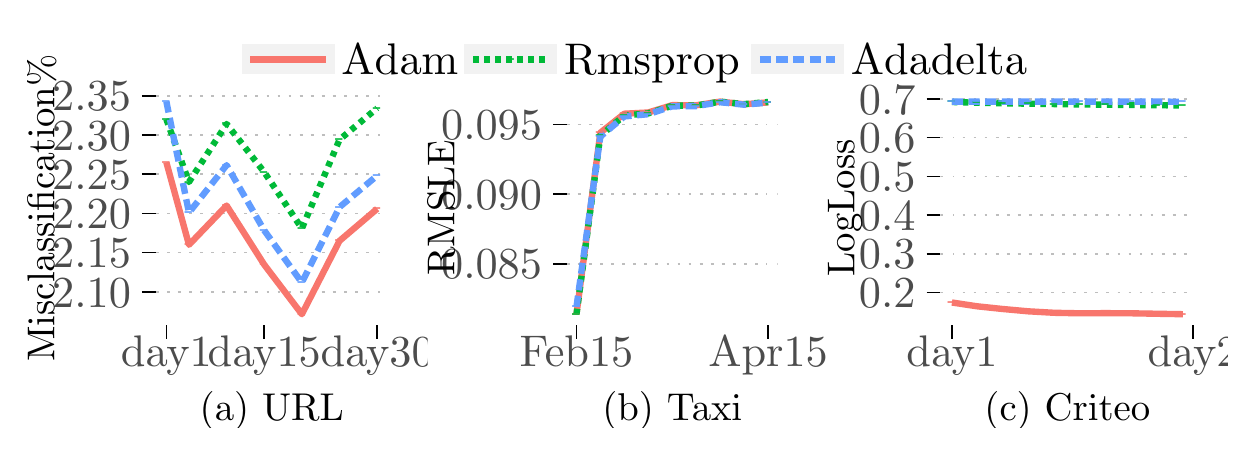
\begin{tikzpicture}[x=1pt,y=1pt]
\definecolor{fillColor}{RGB}{255,255,255}
\path[use as bounding box,fill=fillColor,fill opacity=0.00] (0,0) rectangle (433.62,144.54);
\begin{scope}
\path[clip] (  0.00,  0.00) rectangle (433.62,144.54);
\definecolor{fillColor}{RGB}{255,255,255}

\path[fill=fillColor] ( 67.06,121.66) rectangle (366.56,144.54);
\end{scope}
\begin{scope}
\path[clip] (  0.00,  0.00) rectangle (433.62,144.54);
\definecolor{drawColor}{RGB}{0,0,0}

\node[text=drawColor,anchor=base west,inner sep=0pt, outer sep=0pt, scale=  0.00] at ( 72.75,133.10) {Adaptation};
\end{scope}
\begin{scope}
\path[clip] (  0.00,  0.00) rectangle (433.62,144.54);
\definecolor{drawColor}{RGB}{255,255,255}
\definecolor{fillColor}{gray}{0.95}

\path[draw=drawColor,line width= 0.6pt,line join=round,line cap=round,fill=fillColor] ( 77.09,127.35) rectangle (111.23,138.85);
\end{scope}
\begin{scope}
\path[clip] (  0.00,  0.00) rectangle (433.62,144.54);
\definecolor{drawColor}{RGB}{248,118,109}

\path[draw=drawColor,line width= 2.3pt,line join=round] ( 80.51,133.10) -- (107.82,133.10);
\end{scope}
\begin{scope}
\path[clip] (  0.00,  0.00) rectangle (433.62,144.54);
\definecolor{drawColor}{RGB}{248,118,109}

\node[text=drawColor,anchor=base,inner sep=0pt, outer sep=0pt, scale=  1.00] at ( 94.16,130.94) {-};
\end{scope}
\begin{scope}
\path[clip] (  0.00,  0.00) rectangle (433.62,144.54);
\definecolor{drawColor}{RGB}{255,255,255}
\definecolor{fillColor}{gray}{0.95}

\path[draw=drawColor,line width= 0.6pt,line join=round,line cap=round,fill=fillColor] (157.52,127.35) rectangle (191.67,138.85);
\end{scope}
\begin{scope}
\path[clip] (  0.00,  0.00) rectangle (433.62,144.54);
\definecolor{drawColor}{RGB}{0,186,56}

\path[draw=drawColor,line width= 2.3pt,dash pattern=on 2pt off 2pt ,line join=round] (160.94,133.10) -- (188.25,133.10);
\end{scope}
\begin{scope}
\path[clip] (  0.00,  0.00) rectangle (433.62,144.54);
\definecolor{drawColor}{RGB}{0,186,56}

\node[text=drawColor,anchor=base,inner sep=0pt, outer sep=0pt, scale=  1.00] at (174.60,130.94) {-};
\end{scope}
\begin{scope}
\path[clip] (  0.00,  0.00) rectangle (433.62,144.54);
\definecolor{drawColor}{RGB}{255,255,255}
\definecolor{fillColor}{gray}{0.95}

\path[draw=drawColor,line width= 0.6pt,line join=round,line cap=round,fill=fillColor] (261.15,127.35) rectangle (295.30,138.85);
\end{scope}
\begin{scope}
\path[clip] (  0.00,  0.00) rectangle (433.62,144.54);
\definecolor{drawColor}{RGB}{97,156,255}

\path[draw=drawColor,line width= 2.3pt,dash pattern=on 4pt off 2pt ,line join=round] (264.57,133.10) -- (291.88,133.10);
\end{scope}
\begin{scope}
\path[clip] (  0.00,  0.00) rectangle (433.62,144.54);
\definecolor{drawColor}{RGB}{97,156,255}

\node[text=drawColor,anchor=base,inner sep=0pt, outer sep=0pt, scale=  1.00] at (278.22,130.94) {-};
\end{scope}
\begin{scope}
\path[clip] (  0.00,  0.00) rectangle (433.62,144.54);
\definecolor{drawColor}{RGB}{0,0,0}

\node[text=drawColor,anchor=base west,inner sep=0pt, outer sep=0pt, scale=  1.60] at (113.40,127.59) {Adam};
\end{scope}
\begin{scope}
\path[clip] (  0.00,  0.00) rectangle (433.62,144.54);
\definecolor{drawColor}{RGB}{0,0,0}

\node[text=drawColor,anchor=base west,inner sep=0pt, outer sep=0pt, scale=  1.60] at (193.84,127.59) {Rmsprop};
\end{scope}
\begin{scope}
\path[clip] (  0.00,  0.00) rectangle (433.62,144.54);
\definecolor{drawColor}{RGB}{0,0,0}

\node[text=drawColor,anchor=base west,inner sep=0pt, outer sep=0pt, scale=  1.60] at (297.46,127.59) {Adadelta};
\end{scope}
\begin{scope}
\path[clip] (  0.00,  0.00) rectangle (144.54,121.66);
\definecolor{drawColor}{RGB}{255,255,255}
\definecolor{fillColor}{RGB}{255,255,255}

\path[draw=drawColor,line width= 0.6pt,line join=round,line cap=round,fill=fillColor] (  0.00,  0.00) rectangle (144.54,121.66);
\end{scope}
\begin{scope}
\path[clip] ( 46.31, 37.15) rectangle (130.09,121.66);
\definecolor{fillColor}{RGB}{255,255,255}

\path[fill=fillColor] ( 46.31, 37.15) rectangle (130.09,121.66);
\definecolor{drawColor}{RGB}{255,255,255}

\path[draw=drawColor,line width= 0.3pt,line join=round] ( 46.31, 41.99) --
	(130.09, 41.99);

\path[draw=drawColor,line width= 0.3pt,line join=round] ( 46.31, 56.16) --
	(130.09, 56.16);

\path[draw=drawColor,line width= 0.3pt,line join=round] ( 46.31, 70.34) --
	(130.09, 70.34);

\path[draw=drawColor,line width= 0.3pt,line join=round] ( 46.31, 84.51) --
	(130.09, 84.51);

\path[draw=drawColor,line width= 0.3pt,line join=round] ( 46.31, 98.69) --
	(130.09, 98.69);

\path[draw=drawColor,line width= 0.3pt,line join=round] ( 46.31,112.86) --
	(130.09,112.86);

\path[draw=drawColor,line width= 0.3pt,line join=round] ( 67.80, 37.15) --
	( 67.80,121.66);

\path[draw=drawColor,line width= 0.3pt,line join=round] (105.88, 37.15) --
	(105.88,121.66);
\definecolor{drawColor}{RGB}{190,190,190}

\path[draw=drawColor,line width= 0.6pt,dash pattern=on 1pt off 3pt ,line join=round] ( 46.31, 49.08) --
	(130.09, 49.08);

\path[draw=drawColor,line width= 0.6pt,dash pattern=on 1pt off 3pt ,line join=round] ( 46.31, 63.25) --
	(130.09, 63.25);

\path[draw=drawColor,line width= 0.6pt,dash pattern=on 1pt off 3pt ,line join=round] ( 46.31, 77.42) --
	(130.09, 77.42);

\path[draw=drawColor,line width= 0.6pt,dash pattern=on 1pt off 3pt ,line join=round] ( 46.31, 91.60) --
	(130.09, 91.60);

\path[draw=drawColor,line width= 0.6pt,dash pattern=on 1pt off 3pt ,line join=round] ( 46.31,105.77) --
	(130.09,105.77);

\path[draw=drawColor,line width= 0.6pt,dash pattern=on 1pt off 3pt ,line join=round] ( 46.31,119.95) --
	(130.09,119.95);
\definecolor{drawColor}{RGB}{255,255,255}

\path[draw=drawColor,line width= 0.6pt,line join=round] ( 50.12, 37.15) --
	( 50.12,121.66);

\path[draw=drawColor,line width= 0.6pt,line join=round] ( 85.48, 37.15) --
	( 85.48,121.66);

\path[draw=drawColor,line width= 0.6pt,line join=round] (126.28, 37.15) --
	(126.28,121.66);
\definecolor{drawColor}{RGB}{248,118,109}

\path[draw=drawColor,line width= 2.3pt,line join=round] ( 50.12, 95.85) --
	( 58.28, 66.08) --
	( 71.88, 80.26) --
	( 85.48, 58.90) --
	( 99.08, 41.00) --
	(112.68, 67.50) --
	(126.28, 79.08);
\definecolor{drawColor}{RGB}{0,186,56}

\path[draw=drawColor,line width= 2.3pt,dash pattern=on 2pt off 2pt ,line join=round] ( 50.12,111.44) --
	( 58.28, 88.76) --
	( 71.88,109.74) --
	( 85.48, 92.35) --
	( 99.08, 71.97) --
	(112.68,104.07) --
	(126.28,115.46);
\definecolor{drawColor}{RGB}{97,156,255}

\path[draw=drawColor,line width= 2.3pt,dash pattern=on 4pt off 2pt ,line join=round] ( 50.12,117.82) --
	( 58.28, 77.71) --
	( 71.88, 94.86) --
	( 85.48, 71.28) --
	( 99.08, 52.41) --
	(112.68, 79.69) --
	(126.28, 91.08);
\definecolor{drawColor}{RGB}{248,118,109}

\node[text=drawColor,anchor=base,inner sep=0pt, outer sep=0pt, scale=  1.00] at ( 50.12, 93.69) {-};

\node[text=drawColor,anchor=base,inner sep=0pt, outer sep=0pt, scale=  1.00] at ( 58.28, 63.92) {-};

\node[text=drawColor,anchor=base,inner sep=0pt, outer sep=0pt, scale=  1.00] at ( 71.88, 78.10) {-};

\node[text=drawColor,anchor=base,inner sep=0pt, outer sep=0pt, scale=  1.00] at ( 85.48, 56.74) {-};

\node[text=drawColor,anchor=base,inner sep=0pt, outer sep=0pt, scale=  1.00] at ( 99.08, 38.83) {-};

\node[text=drawColor,anchor=base,inner sep=0pt, outer sep=0pt, scale=  1.00] at (112.68, 65.34) {-};

\node[text=drawColor,anchor=base,inner sep=0pt, outer sep=0pt, scale=  1.00] at (126.28, 76.92) {-};
\definecolor{drawColor}{RGB}{0,186,56}

\node[text=drawColor,anchor=base,inner sep=0pt, outer sep=0pt, scale=  1.00] at ( 50.12,109.28) {-};

\node[text=drawColor,anchor=base,inner sep=0pt, outer sep=0pt, scale=  1.00] at ( 58.28, 86.60) {-};

\node[text=drawColor,anchor=base,inner sep=0pt, outer sep=0pt, scale=  1.00] at ( 71.88,107.58) {-};

\node[text=drawColor,anchor=base,inner sep=0pt, outer sep=0pt, scale=  1.00] at ( 85.48, 90.19) {-};

\node[text=drawColor,anchor=base,inner sep=0pt, outer sep=0pt, scale=  1.00] at ( 99.08, 69.80) {-};

\node[text=drawColor,anchor=base,inner sep=0pt, outer sep=0pt, scale=  1.00] at (112.68,101.91) {-};

\node[text=drawColor,anchor=base,inner sep=0pt, outer sep=0pt, scale=  1.00] at (126.28,113.30) {-};
\definecolor{drawColor}{RGB}{97,156,255}

\node[text=drawColor,anchor=base,inner sep=0pt, outer sep=0pt, scale=  1.00] at ( 50.12,115.66) {-};

\node[text=drawColor,anchor=base,inner sep=0pt, outer sep=0pt, scale=  1.00] at ( 58.28, 75.54) {-};

\node[text=drawColor,anchor=base,inner sep=0pt, outer sep=0pt, scale=  1.00] at ( 71.88, 92.70) {-};

\node[text=drawColor,anchor=base,inner sep=0pt, outer sep=0pt, scale=  1.00] at ( 85.48, 69.12) {-};

\node[text=drawColor,anchor=base,inner sep=0pt, outer sep=0pt, scale=  1.00] at ( 99.08, 50.24) {-};

\node[text=drawColor,anchor=base,inner sep=0pt, outer sep=0pt, scale=  1.00] at (112.68, 77.53) {-};

\node[text=drawColor,anchor=base,inner sep=0pt, outer sep=0pt, scale=  1.00] at (126.28, 88.92) {-};
\end{scope}
\begin{scope}
\path[clip] (  0.00,  0.00) rectangle (433.62,144.54);
\definecolor{drawColor}{gray}{0.30}

\node[text=drawColor,anchor=base east,inner sep=0pt, outer sep=0pt, scale=  1.60] at ( 37.31, 43.57) {2.10};

\node[text=drawColor,anchor=base east,inner sep=0pt, outer sep=0pt, scale=  1.60] at ( 37.31, 57.74) {2.15};

\node[text=drawColor,anchor=base east,inner sep=0pt, outer sep=0pt, scale=  1.60] at ( 37.31, 71.91) {2.20};

\node[text=drawColor,anchor=base east,inner sep=0pt, outer sep=0pt, scale=  1.60] at ( 37.31, 86.09) {2.25};

\node[text=drawColor,anchor=base east,inner sep=0pt, outer sep=0pt, scale=  1.60] at ( 37.31,100.26) {2.30};

\node[text=drawColor,anchor=base east,inner sep=0pt, outer sep=0pt, scale=  1.60] at ( 37.31,114.44) {2.35};
\end{scope}
\begin{scope}
\path[clip] (  0.00,  0.00) rectangle (433.62,144.54);
\definecolor{drawColor}{RGB}{0,0,0}

\path[draw=drawColor,line width= 0.6pt,line join=round] ( 41.31, 49.08) --
	( 46.31, 49.08);

\path[draw=drawColor,line width= 0.6pt,line join=round] ( 41.31, 63.25) --
	( 46.31, 63.25);

\path[draw=drawColor,line width= 0.6pt,line join=round] ( 41.31, 77.42) --
	( 46.31, 77.42);

\path[draw=drawColor,line width= 0.6pt,line join=round] ( 41.31, 91.60) --
	( 46.31, 91.60);

\path[draw=drawColor,line width= 0.6pt,line join=round] ( 41.31,105.77) --
	( 46.31,105.77);

\path[draw=drawColor,line width= 0.6pt,line join=round] ( 41.31,119.95) --
	( 46.31,119.95);
\end{scope}
\begin{scope}
\path[clip] (  0.00,  0.00) rectangle (433.62,144.54);
\definecolor{drawColor}{RGB}{0,0,0}

\path[draw=drawColor,line width= 0.6pt,line join=round] ( 50.12, 32.15) --
	( 50.12, 37.15);

\path[draw=drawColor,line width= 0.6pt,line join=round] ( 85.48, 32.15) --
	( 85.48, 37.15);

\path[draw=drawColor,line width= 0.6pt,line join=round] (126.28, 32.15) --
	(126.28, 37.15);
\end{scope}
\begin{scope}
\path[clip] (  0.00,  0.00) rectangle (433.62,144.54);
\definecolor{drawColor}{gray}{0.30}

\node[text=drawColor,anchor=base,inner sep=0pt, outer sep=0pt, scale=  1.60] at ( 50.12, 22.14) {day1};

\node[text=drawColor,anchor=base,inner sep=0pt, outer sep=0pt, scale=  1.60] at ( 85.48, 22.14) {day15};

\node[text=drawColor,anchor=base,inner sep=0pt, outer sep=0pt, scale=  1.60] at (126.28, 22.14) {day30};
\end{scope}
\begin{scope}
\path[clip] (  0.00,  0.00) rectangle (433.62,144.54);
\definecolor{drawColor}{RGB}{0,0,0}

\node[text=drawColor,anchor=base,inner sep=0pt, outer sep=0pt, scale=  1.40] at ( 88.20,  2.49) {(a) URL};
\end{scope}
\begin{scope}
\path[clip] (  0.00,  0.00) rectangle (433.62,144.54);
\definecolor{drawColor}{RGB}{0,0,0}

\node[text=drawColor,rotate= 90.00,anchor=base,inner sep=0pt, outer sep=0pt, scale=  1.40] at (  9.64, 79.41) {Misclassification\%};
\end{scope}
\begin{scope}
\path[clip] (144.54,  0.00) rectangle (289.08,121.66);
\definecolor{drawColor}{RGB}{255,255,255}
\definecolor{fillColor}{RGB}{255,255,255}

\path[draw=drawColor,line width= 0.6pt,line join=round,line cap=round,fill=fillColor] (144.54,  0.00) rectangle (289.08,121.66);
\end{scope}
\begin{scope}
\path[clip] (194.85, 37.15) rectangle (271.01,121.66);
\definecolor{fillColor}{RGB}{255,255,255}

\path[fill=fillColor] (194.85, 37.15) rectangle (271.01,121.66);
\definecolor{drawColor}{RGB}{255,255,255}

\path[draw=drawColor,line width= 0.3pt,line join=round] (194.85, 46.69) --
	(271.01, 46.69);

\path[draw=drawColor,line width= 0.3pt,line join=round] (194.85, 71.81) --
	(271.01, 71.81);

\path[draw=drawColor,line width= 0.3pt,line join=round] (194.85, 96.93) --
	(271.01, 96.93);

\path[draw=drawColor,line width= 0.3pt,line join=round] (232.93, 37.15) --
	(232.93,121.66);
\definecolor{drawColor}{RGB}{190,190,190}

\path[draw=drawColor,line width= 0.6pt,dash pattern=on 1pt off 3pt ,line join=round] (194.85, 59.25) --
	(271.01, 59.25);

\path[draw=drawColor,line width= 0.6pt,dash pattern=on 1pt off 3pt ,line join=round] (194.85, 84.37) --
	(271.01, 84.37);

\path[draw=drawColor,line width= 0.6pt,dash pattern=on 1pt off 3pt ,line join=round] (194.85,109.49) --
	(271.01,109.49);
\definecolor{drawColor}{RGB}{255,255,255}

\path[draw=drawColor,line width= 0.6pt,line join=round] (198.31, 37.15) --
	(198.31,121.66);

\path[draw=drawColor,line width= 0.6pt,line join=round] (267.55, 37.15) --
	(267.55,121.66);
\definecolor{drawColor}{RGB}{248,118,109}

\path[draw=drawColor,line width= 2.3pt,line join=round] (198.31, 41.06) --
	(206.93,106.58) --
	(215.59,113.45) --
	(224.25,113.89) --
	(232.91,116.54) --
	(241.57,116.50) --
	(250.23,117.82) --
	(258.89,116.86) --
	(267.55,117.55);
\definecolor{drawColor}{RGB}{0,186,56}

\path[draw=drawColor,line width= 2.3pt,dash pattern=on 2pt off 2pt ,line join=round] (198.31, 41.00) --
	(206.93,105.43) --
	(215.59,112.82) --
	(224.25,113.56) --
	(232.91,116.33) --
	(241.57,116.39) --
	(250.23,117.80) --
	(258.89,116.91) --
	(267.55,117.68);
\definecolor{drawColor}{RGB}{97,156,255}

\path[draw=drawColor,line width= 2.3pt,dash pattern=on 4pt off 2pt ,line join=round] (198.31, 43.71) --
	(206.93,105.17) --
	(215.59,112.46) --
	(224.25,113.27) --
	(232.91,116.10) --
	(241.57,116.20) --
	(250.23,117.60) --
	(258.89,116.71) --
	(267.55,117.46);
\definecolor{drawColor}{RGB}{248,118,109}

\node[text=drawColor,anchor=base,inner sep=0pt, outer sep=0pt, scale=  1.00] at (198.31, 38.90) {-};

\node[text=drawColor,anchor=base,inner sep=0pt, outer sep=0pt, scale=  1.00] at (206.93,104.42) {-};

\node[text=drawColor,anchor=base,inner sep=0pt, outer sep=0pt, scale=  1.00] at (215.59,111.29) {-};

\node[text=drawColor,anchor=base,inner sep=0pt, outer sep=0pt, scale=  1.00] at (224.25,111.73) {-};

\node[text=drawColor,anchor=base,inner sep=0pt, outer sep=0pt, scale=  1.00] at (232.91,114.37) {-};

\node[text=drawColor,anchor=base,inner sep=0pt, outer sep=0pt, scale=  1.00] at (241.57,114.33) {-};

\node[text=drawColor,anchor=base,inner sep=0pt, outer sep=0pt, scale=  1.00] at (250.23,115.66) {-};

\node[text=drawColor,anchor=base,inner sep=0pt, outer sep=0pt, scale=  1.00] at (258.89,114.69) {-};

\node[text=drawColor,anchor=base,inner sep=0pt, outer sep=0pt, scale=  1.00] at (267.55,115.39) {-};
\definecolor{drawColor}{RGB}{0,186,56}

\node[text=drawColor,anchor=base,inner sep=0pt, outer sep=0pt, scale=  1.00] at (198.31, 38.83) {-};

\node[text=drawColor,anchor=base,inner sep=0pt, outer sep=0pt, scale=  1.00] at (206.93,103.26) {-};

\node[text=drawColor,anchor=base,inner sep=0pt, outer sep=0pt, scale=  1.00] at (215.59,110.66) {-};

\node[text=drawColor,anchor=base,inner sep=0pt, outer sep=0pt, scale=  1.00] at (224.25,111.40) {-};

\node[text=drawColor,anchor=base,inner sep=0pt, outer sep=0pt, scale=  1.00] at (232.91,114.17) {-};

\node[text=drawColor,anchor=base,inner sep=0pt, outer sep=0pt, scale=  1.00] at (241.57,114.23) {-};

\node[text=drawColor,anchor=base,inner sep=0pt, outer sep=0pt, scale=  1.00] at (250.23,115.63) {-};

\node[text=drawColor,anchor=base,inner sep=0pt, outer sep=0pt, scale=  1.00] at (258.89,114.74) {-};

\node[text=drawColor,anchor=base,inner sep=0pt, outer sep=0pt, scale=  1.00] at (267.55,115.51) {-};
\definecolor{drawColor}{RGB}{97,156,255}

\node[text=drawColor,anchor=base,inner sep=0pt, outer sep=0pt, scale=  1.00] at (198.31, 41.54) {-};

\node[text=drawColor,anchor=base,inner sep=0pt, outer sep=0pt, scale=  1.00] at (206.93,103.01) {-};

\node[text=drawColor,anchor=base,inner sep=0pt, outer sep=0pt, scale=  1.00] at (215.59,110.30) {-};

\node[text=drawColor,anchor=base,inner sep=0pt, outer sep=0pt, scale=  1.00] at (224.25,111.10) {-};

\node[text=drawColor,anchor=base,inner sep=0pt, outer sep=0pt, scale=  1.00] at (232.91,113.94) {-};

\node[text=drawColor,anchor=base,inner sep=0pt, outer sep=0pt, scale=  1.00] at (241.57,114.04) {-};

\node[text=drawColor,anchor=base,inner sep=0pt, outer sep=0pt, scale=  1.00] at (250.23,115.43) {-};

\node[text=drawColor,anchor=base,inner sep=0pt, outer sep=0pt, scale=  1.00] at (258.89,114.55) {-};

\node[text=drawColor,anchor=base,inner sep=0pt, outer sep=0pt, scale=  1.00] at (267.55,115.30) {-};
\end{scope}
\begin{scope}
\path[clip] (  0.00,  0.00) rectangle (433.62,144.54);
\definecolor{drawColor}{gray}{0.30}

\node[text=drawColor,anchor=base east,inner sep=0pt, outer sep=0pt, scale=  1.60] at (185.85, 53.74) {0.085};

\node[text=drawColor,anchor=base east,inner sep=0pt, outer sep=0pt, scale=  1.60] at (185.85, 78.86) {0.090};

\node[text=drawColor,anchor=base east,inner sep=0pt, outer sep=0pt, scale=  1.60] at (185.85,103.98) {0.095};
\end{scope}
\begin{scope}
\path[clip] (  0.00,  0.00) rectangle (433.62,144.54);
\definecolor{drawColor}{RGB}{0,0,0}

\path[draw=drawColor,line width= 0.6pt,line join=round] (189.85, 59.25) --
	(194.85, 59.25);

\path[draw=drawColor,line width= 0.6pt,line join=round] (189.85, 84.37) --
	(194.85, 84.37);

\path[draw=drawColor,line width= 0.6pt,line join=round] (189.85,109.49) --
	(194.85,109.49);
\end{scope}
\begin{scope}
\path[clip] (  0.00,  0.00) rectangle (433.62,144.54);
\definecolor{drawColor}{RGB}{0,0,0}

\path[draw=drawColor,line width= 0.6pt,line join=round] (198.31, 32.15) --
	(198.31, 37.15);

\path[draw=drawColor,line width= 0.6pt,line join=round] (267.55, 32.15) --
	(267.55, 37.15);
\end{scope}
\begin{scope}
\path[clip] (  0.00,  0.00) rectangle (433.62,144.54);
\definecolor{drawColor}{gray}{0.30}

\node[text=drawColor,anchor=base,inner sep=0pt, outer sep=0pt, scale=  1.60] at (198.31, 22.14) {Feb15};

\node[text=drawColor,anchor=base,inner sep=0pt, outer sep=0pt, scale=  1.60] at (267.55, 22.14) {Apr15};
\end{scope}
\begin{scope}
\path[clip] (  0.00,  0.00) rectangle (433.62,144.54);
\definecolor{drawColor}{RGB}{0,0,0}

\node[text=drawColor,anchor=base,inner sep=0pt, outer sep=0pt, scale=  1.40] at (232.93,  2.49) {(b) Taxi};
\end{scope}
\begin{scope}
\path[clip] (  0.00,  0.00) rectangle (433.62,144.54);
\definecolor{drawColor}{RGB}{0,0,0}

\node[text=drawColor,rotate= 90.00,anchor=base,inner sep=0pt, outer sep=0pt, scale=  1.40] at (154.18, 79.41) {RMSLE};
\end{scope}
\begin{scope}
\path[clip] (289.08,  0.00) rectangle (433.62,121.66);
\definecolor{drawColor}{RGB}{255,255,255}
\definecolor{fillColor}{RGB}{255,255,255}

\path[draw=drawColor,line width= 0.6pt,line join=round,line cap=round,fill=fillColor] (289.08,  0.00) rectangle (433.62,121.66);
\end{scope}
\begin{scope}
\path[clip] (329.81, 37.15) rectangle (421.57,121.66);
\definecolor{fillColor}{RGB}{255,255,255}

\path[fill=fillColor] (329.81, 37.15) rectangle (421.57,121.66);
\definecolor{drawColor}{RGB}{255,255,255}

\path[draw=drawColor,line width= 0.3pt,line join=round] (329.81, 41.88) --
	(421.57, 41.88);

\path[draw=drawColor,line width= 0.3pt,line join=round] (329.81, 55.86) --
	(421.57, 55.86);

\path[draw=drawColor,line width= 0.3pt,line join=round] (329.81, 69.84) --
	(421.57, 69.84);

\path[draw=drawColor,line width= 0.3pt,line join=round] (329.81, 83.83) --
	(421.57, 83.83);

\path[draw=drawColor,line width= 0.3pt,line join=round] (329.81, 97.81) --
	(421.57, 97.81);

\path[draw=drawColor,line width= 0.3pt,line join=round] (329.81,111.79) --
	(421.57,111.79);

\path[draw=drawColor,line width= 0.3pt,line join=round] (377.55, 37.15) --
	(377.55,121.66);
\definecolor{drawColor}{RGB}{190,190,190}

\path[draw=drawColor,line width= 0.6pt,dash pattern=on 1pt off 3pt ,line join=round] (329.81, 48.87) --
	(421.57, 48.87);

\path[draw=drawColor,line width= 0.6pt,dash pattern=on 1pt off 3pt ,line join=round] (329.81, 62.85) --
	(421.57, 62.85);

\path[draw=drawColor,line width= 0.6pt,dash pattern=on 1pt off 3pt ,line join=round] (329.81, 76.83) --
	(421.57, 76.83);

\path[draw=drawColor,line width= 0.6pt,dash pattern=on 1pt off 3pt ,line join=round] (329.81, 90.82) --
	(421.57, 90.82);

\path[draw=drawColor,line width= 0.6pt,dash pattern=on 1pt off 3pt ,line join=round] (329.81,104.80) --
	(421.57,104.80);

\path[draw=drawColor,line width= 0.6pt,dash pattern=on 1pt off 3pt ,line join=round] (329.81,118.78) --
	(421.57,118.78);
\definecolor{drawColor}{RGB}{255,255,255}

\path[draw=drawColor,line width= 0.6pt,line join=round] (333.98, 37.15) --
	(333.98,121.66);

\path[draw=drawColor,line width= 0.6pt,line join=round] (421.12, 37.15) --
	(421.12,121.66);
\definecolor{drawColor}{RGB}{248,118,109}

\path[draw=drawColor,line width= 2.3pt,line join=round] (333.98, 45.23) --
	(343.05, 43.86) --
	(352.34, 42.88) --
	(361.63, 42.04) --
	(370.93, 41.51) --
	(380.22, 41.33) --
	(389.52, 41.38) --
	(398.81, 41.33) --
	(408.11, 41.16) --
	(417.40, 41.00);
\definecolor{drawColor}{RGB}{0,186,56}

\path[draw=drawColor,line width= 2.3pt,dash pattern=on 2pt off 2pt ,line join=round] (333.98,117.68) --
	(343.05,117.43) --
	(352.34,117.23) --
	(361.63,117.07) --
	(370.93,116.93) --
	(380.22,116.80) --
	(389.52,116.70) --
	(398.81,116.60) --
	(408.11,116.51) --
	(417.40,116.43);
\definecolor{drawColor}{RGB}{97,156,255}

\path[draw=drawColor,line width= 2.3pt,dash pattern=on 4pt off 2pt ,line join=round] (333.98,117.82) --
	(343.05,117.82) --
	(352.34,117.82) --
	(361.63,117.81) --
	(370.93,117.81) --
	(380.22,117.81) --
	(389.52,117.80) --
	(398.81,117.80) --
	(408.11,117.80) --
	(417.40,117.79);
\definecolor{drawColor}{RGB}{248,118,109}

\node[text=drawColor,anchor=base,inner sep=0pt, outer sep=0pt, scale=  1.00] at (333.98, 43.07) {-};

\node[text=drawColor,anchor=base,inner sep=0pt, outer sep=0pt, scale=  1.00] at (343.05, 41.70) {-};

\node[text=drawColor,anchor=base,inner sep=0pt, outer sep=0pt, scale=  1.00] at (352.34, 40.72) {-};

\node[text=drawColor,anchor=base,inner sep=0pt, outer sep=0pt, scale=  1.00] at (361.63, 39.88) {-};

\node[text=drawColor,anchor=base,inner sep=0pt, outer sep=0pt, scale=  1.00] at (370.93, 39.34) {-};

\node[text=drawColor,anchor=base,inner sep=0pt, outer sep=0pt, scale=  1.00] at (380.22, 39.16) {-};

\node[text=drawColor,anchor=base,inner sep=0pt, outer sep=0pt, scale=  1.00] at (389.52, 39.22) {-};

\node[text=drawColor,anchor=base,inner sep=0pt, outer sep=0pt, scale=  1.00] at (398.81, 39.16) {-};

\node[text=drawColor,anchor=base,inner sep=0pt, outer sep=0pt, scale=  1.00] at (408.11, 38.99) {-};

\node[text=drawColor,anchor=base,inner sep=0pt, outer sep=0pt, scale=  1.00] at (417.40, 38.83) {-};
\definecolor{drawColor}{RGB}{0,186,56}

\node[text=drawColor,anchor=base,inner sep=0pt, outer sep=0pt, scale=  1.00] at (333.98,115.52) {-};

\node[text=drawColor,anchor=base,inner sep=0pt, outer sep=0pt, scale=  1.00] at (343.05,115.27) {-};

\node[text=drawColor,anchor=base,inner sep=0pt, outer sep=0pt, scale=  1.00] at (352.34,115.07) {-};

\node[text=drawColor,anchor=base,inner sep=0pt, outer sep=0pt, scale=  1.00] at (361.63,114.91) {-};

\node[text=drawColor,anchor=base,inner sep=0pt, outer sep=0pt, scale=  1.00] at (370.93,114.76) {-};

\node[text=drawColor,anchor=base,inner sep=0pt, outer sep=0pt, scale=  1.00] at (380.22,114.64) {-};

\node[text=drawColor,anchor=base,inner sep=0pt, outer sep=0pt, scale=  1.00] at (389.52,114.53) {-};

\node[text=drawColor,anchor=base,inner sep=0pt, outer sep=0pt, scale=  1.00] at (398.81,114.44) {-};

\node[text=drawColor,anchor=base,inner sep=0pt, outer sep=0pt, scale=  1.00] at (408.11,114.35) {-};

\node[text=drawColor,anchor=base,inner sep=0pt, outer sep=0pt, scale=  1.00] at (417.40,114.27) {-};
\definecolor{drawColor}{RGB}{97,156,255}

\node[text=drawColor,anchor=base,inner sep=0pt, outer sep=0pt, scale=  1.00] at (333.98,115.66) {-};

\node[text=drawColor,anchor=base,inner sep=0pt, outer sep=0pt, scale=  1.00] at (343.05,115.66) {-};

\node[text=drawColor,anchor=base,inner sep=0pt, outer sep=0pt, scale=  1.00] at (352.34,115.65) {-};

\node[text=drawColor,anchor=base,inner sep=0pt, outer sep=0pt, scale=  1.00] at (361.63,115.65) {-};

\node[text=drawColor,anchor=base,inner sep=0pt, outer sep=0pt, scale=  1.00] at (370.93,115.65) {-};

\node[text=drawColor,anchor=base,inner sep=0pt, outer sep=0pt, scale=  1.00] at (380.22,115.64) {-};

\node[text=drawColor,anchor=base,inner sep=0pt, outer sep=0pt, scale=  1.00] at (389.52,115.64) {-};

\node[text=drawColor,anchor=base,inner sep=0pt, outer sep=0pt, scale=  1.00] at (398.81,115.64) {-};

\node[text=drawColor,anchor=base,inner sep=0pt, outer sep=0pt, scale=  1.00] at (408.11,115.63) {-};

\node[text=drawColor,anchor=base,inner sep=0pt, outer sep=0pt, scale=  1.00] at (417.40,115.63) {-};
\end{scope}
\begin{scope}
\path[clip] (  0.00,  0.00) rectangle (433.62,144.54);
\definecolor{drawColor}{gray}{0.30}

\node[text=drawColor,anchor=base east,inner sep=0pt, outer sep=0pt, scale=  1.60] at (320.81, 43.36) {0.2};

\node[text=drawColor,anchor=base east,inner sep=0pt, outer sep=0pt, scale=  1.60] at (320.81, 57.34) {0.3};

\node[text=drawColor,anchor=base east,inner sep=0pt, outer sep=0pt, scale=  1.60] at (320.81, 71.32) {0.4};

\node[text=drawColor,anchor=base east,inner sep=0pt, outer sep=0pt, scale=  1.60] at (320.81, 85.31) {0.5};

\node[text=drawColor,anchor=base east,inner sep=0pt, outer sep=0pt, scale=  1.60] at (320.81, 99.29) {0.6};

\node[text=drawColor,anchor=base east,inner sep=0pt, outer sep=0pt, scale=  1.60] at (320.81,113.27) {0.7};
\end{scope}
\begin{scope}
\path[clip] (  0.00,  0.00) rectangle (433.62,144.54);
\definecolor{drawColor}{RGB}{0,0,0}

\path[draw=drawColor,line width= 0.6pt,line join=round] (324.81, 48.87) --
	(329.81, 48.87);

\path[draw=drawColor,line width= 0.6pt,line join=round] (324.81, 62.85) --
	(329.81, 62.85);

\path[draw=drawColor,line width= 0.6pt,line join=round] (324.81, 76.83) --
	(329.81, 76.83);

\path[draw=drawColor,line width= 0.6pt,line join=round] (324.81, 90.82) --
	(329.81, 90.82);

\path[draw=drawColor,line width= 0.6pt,line join=round] (324.81,104.80) --
	(329.81,104.80);

\path[draw=drawColor,line width= 0.6pt,line join=round] (324.81,118.78) --
	(329.81,118.78);
\end{scope}
\begin{scope}
\path[clip] (  0.00,  0.00) rectangle (433.62,144.54);
\definecolor{drawColor}{RGB}{0,0,0}

\path[draw=drawColor,line width= 0.6pt,line join=round] (333.98, 32.15) --
	(333.98, 37.15);

\path[draw=drawColor,line width= 0.6pt,line join=round] (421.12, 32.15) --
	(421.12, 37.15);
\end{scope}
\begin{scope}
\path[clip] (  0.00,  0.00) rectangle (433.62,144.54);
\definecolor{drawColor}{gray}{0.30}

\node[text=drawColor,anchor=base,inner sep=0pt, outer sep=0pt, scale=  1.60] at (333.98, 22.14) {day1};

\node[text=drawColor,anchor=base,inner sep=0pt, outer sep=0pt, scale=  1.60] at (421.12, 22.14) {day2};
\end{scope}
\begin{scope}
\path[clip] (  0.00,  0.00) rectangle (433.62,144.54);
\definecolor{drawColor}{RGB}{0,0,0}

\node[text=drawColor,anchor=base,inner sep=0pt, outer sep=0pt, scale=  1.40] at (375.69,  2.49) {(c) Criteo};
\end{scope}
\begin{scope}
\path[clip] (  0.00,  0.00) rectangle (433.62,144.54);
\definecolor{drawColor}{RGB}{0,0,0}

\node[text=drawColor,rotate= 90.00,anchor=base,inner sep=0pt, outer sep=0pt, scale=  1.40] at (298.72, 79.41) {LogLoss};
\end{scope}
\end{tikzpicture}
}
\caption{Result of hyperparameter tuning during initial phases of deployment}
\label{hyper-param-figure}
\end{figure}

\textbf{Sampling Methods.}
The choice of the sampling strategy also affects the proactive training.
Each instance of the proactive training updates the deployed model using the provided sample.
Therefore, the quality of the model after an update is directly related to the quality of the data inside the sample.
We evaluate the effect of three different sampling methods, time-based, window-based, and uniform, on the quality of the deployed model.
\todo[inline]{Exact size}
The sample size is similar to the sample size during the initial training.
Figure \ref{sampling-method-figure} shows the effect of different sampling strategies on the quality of the deployed model.
For the URL dataset, time-based sampling achieves the lowest error rate for the deployed model.
For the URL dataset, the underlying characteristics of the data gradually change over time, as new features are added to the dataset \cite{ma2009identifying}.
A time-based sampling approach is more likely to select the recent items for the proactive training.
As a result, the deployed model performs better on the incoming prediction queries.
Taxi dataset does not contain any known concept drift.
As a result, we observe that different sampling strategies have the same effect on the quality of the deployed model.

Since the existence of concept drift is not always known beforehand, we choose time-based sampling for our deployment platform.
For datasets that contain concept drift, time-based sampling outperforms other sampling strategies, while providing the same performance for datasets without concept drift.

\begin{figure}[!h]
\centering
\resizebox{\columnwidth}{!}{% Created by tikzDevice version 0.11 on 2018-05-19 10:35:13
% !TEX encoding = UTF-8 Unicode
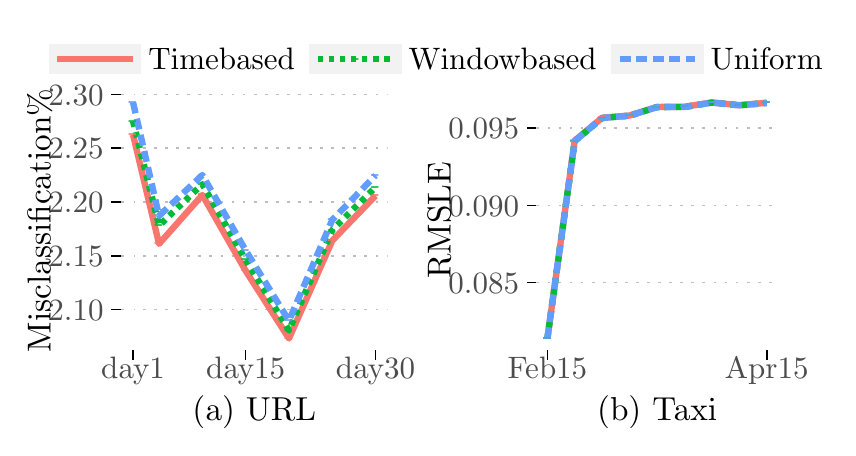
\begin{tikzpicture}[x=1pt,y=1pt]
\definecolor{fillColor}{RGB}{255,255,255}
\path[use as bounding box,fill=fillColor,fill opacity=0.00] (0,0) rectangle (289.08,144.54);
\begin{scope}
\path[clip] (  0.00,  0.00) rectangle (289.08,144.54);
\definecolor{fillColor}{RGB}{255,255,255}

\path[fill=fillColor] ( -2.74,121.78) rectangle (291.82,144.54);
\end{scope}
\begin{scope}
\path[clip] (  0.00,  0.00) rectangle (289.08,144.54);
\definecolor{drawColor}{RGB}{0,0,0}

\node[text=drawColor,anchor=base west,inner sep=0pt, outer sep=0pt, scale=  0.00] at (  2.95,133.16) {Sampling};
\end{scope}
\begin{scope}
\path[clip] (  0.00,  0.00) rectangle (289.08,144.54);
\definecolor{drawColor}{RGB}{255,255,255}
\definecolor{fillColor}{gray}{0.95}

\path[draw=drawColor,line width= 0.6pt,line join=round,line cap=round,fill=fillColor] (  7.28,127.47) rectangle ( 41.43,138.85);
\end{scope}
\begin{scope}
\path[clip] (  0.00,  0.00) rectangle (289.08,144.54);
\definecolor{drawColor}{RGB}{248,118,109}

\path[draw=drawColor,line width= 2.3pt,line join=round] ( 10.70,133.16) -- ( 38.01,133.16);
\end{scope}
\begin{scope}
\path[clip] (  0.00,  0.00) rectangle (289.08,144.54);
\definecolor{drawColor}{RGB}{248,118,109}

\node[text=drawColor,anchor=base,inner sep=0pt, outer sep=0pt, scale=  1.00] at ( 24.36,131.00) {-};
\end{scope}
\begin{scope}
\path[clip] (  0.00,  0.00) rectangle (289.08,144.54);
\definecolor{drawColor}{RGB}{255,255,255}
\definecolor{fillColor}{gray}{0.95}

\path[draw=drawColor,line width= 0.6pt,line join=round,line cap=round,fill=fillColor] (101.38,127.47) rectangle (135.52,138.85);
\end{scope}
\begin{scope}
\path[clip] (  0.00,  0.00) rectangle (289.08,144.54);
\definecolor{drawColor}{RGB}{0,186,56}

\path[draw=drawColor,line width= 2.3pt,dash pattern=on 2pt off 2pt ,line join=round] (104.79,133.16) -- (132.10,133.16);
\end{scope}
\begin{scope}
\path[clip] (  0.00,  0.00) rectangle (289.08,144.54);
\definecolor{drawColor}{RGB}{0,186,56}

\node[text=drawColor,anchor=base,inner sep=0pt, outer sep=0pt, scale=  1.00] at (118.45,131.00) {-};
\end{scope}
\begin{scope}
\path[clip] (  0.00,  0.00) rectangle (289.08,144.54);
\definecolor{drawColor}{RGB}{255,255,255}
\definecolor{fillColor}{gray}{0.95}

\path[draw=drawColor,line width= 0.6pt,line join=round,line cap=round,fill=fillColor] (210.47,127.47) rectangle (244.61,138.85);
\end{scope}
\begin{scope}
\path[clip] (  0.00,  0.00) rectangle (289.08,144.54);
\definecolor{drawColor}{RGB}{97,156,255}

\path[draw=drawColor,line width= 2.3pt,dash pattern=on 4pt off 2pt ,line join=round] (213.88,133.16) -- (241.20,133.16);
\end{scope}
\begin{scope}
\path[clip] (  0.00,  0.00) rectangle (289.08,144.54);
\definecolor{drawColor}{RGB}{97,156,255}

\node[text=drawColor,anchor=base,inner sep=0pt, outer sep=0pt, scale=  1.00] at (227.54,131.00) {-};
\end{scope}
\begin{scope}
\path[clip] (  0.00,  0.00) rectangle (289.08,144.54);
\definecolor{drawColor}{RGB}{0,0,0}

\node[text=drawColor,anchor=base west,inner sep=0pt, outer sep=0pt, scale=  1.12] at ( 43.60,129.30) {Timebased};
\end{scope}
\begin{scope}
\path[clip] (  0.00,  0.00) rectangle (289.08,144.54);
\definecolor{drawColor}{RGB}{0,0,0}

\node[text=drawColor,anchor=base west,inner sep=0pt, outer sep=0pt, scale=  1.12] at (137.69,129.30) {Windowbased};
\end{scope}
\begin{scope}
\path[clip] (  0.00,  0.00) rectangle (289.08,144.54);
\definecolor{drawColor}{RGB}{0,0,0}

\node[text=drawColor,anchor=base west,inner sep=0pt, outer sep=0pt, scale=  1.12] at (246.78,129.30) {Uniform};
\end{scope}
\begin{scope}
\path[clip] (  0.00,  0.00) rectangle (144.54,121.78);
\definecolor{drawColor}{RGB}{255,255,255}
\definecolor{fillColor}{RGB}{255,255,255}

\path[draw=drawColor,line width= 0.6pt,line join=round,line cap=round,fill=fillColor] ( -0.00,  0.00) rectangle (144.54,121.78);
\end{scope}
\begin{scope}
\path[clip] ( 33.70, 27.97) rectangle (130.09,121.78);
\definecolor{fillColor}{RGB}{255,255,255}

\path[fill=fillColor] ( 33.70, 27.97) rectangle (130.09,121.78);
\definecolor{drawColor}{RGB}{255,255,255}

\path[draw=drawColor,line width= 0.3pt,line join=round] ( 33.70, 33.01) --
	(130.09, 33.01);

\path[draw=drawColor,line width= 0.3pt,line join=round] ( 33.70, 52.44) --
	(130.09, 52.44);

\path[draw=drawColor,line width= 0.3pt,line join=round] ( 33.70, 71.86) --
	(130.09, 71.86);

\path[draw=drawColor,line width= 0.3pt,line join=round] ( 33.70, 91.29) --
	(130.09, 91.29);

\path[draw=drawColor,line width= 0.3pt,line join=round] ( 33.70,110.71) --
	(130.09,110.71);

\path[draw=drawColor,line width= 0.3pt,line join=round] ( 58.42, 27.97) --
	( 58.42,121.78);

\path[draw=drawColor,line width= 0.3pt,line join=round] (102.23, 27.97) --
	(102.23,121.78);
\definecolor{drawColor}{RGB}{190,190,190}

\path[draw=drawColor,line width= 0.6pt,dash pattern=on 1pt off 3pt ,line join=round] ( 33.70, 42.73) --
	(130.09, 42.73);

\path[draw=drawColor,line width= 0.6pt,dash pattern=on 1pt off 3pt ,line join=round] ( 33.70, 62.15) --
	(130.09, 62.15);

\path[draw=drawColor,line width= 0.6pt,dash pattern=on 1pt off 3pt ,line join=round] ( 33.70, 81.58) --
	(130.09, 81.58);

\path[draw=drawColor,line width= 0.6pt,dash pattern=on 1pt off 3pt ,line join=round] ( 33.70,101.00) --
	(130.09,101.00);

\path[draw=drawColor,line width= 0.6pt,dash pattern=on 1pt off 3pt ,line join=round] ( 33.70,120.43) --
	(130.09,120.43);
\definecolor{drawColor}{RGB}{255,255,255}

\path[draw=drawColor,line width= 0.6pt,line join=round] ( 38.08, 27.97) --
	( 38.08,121.78);

\path[draw=drawColor,line width= 0.6pt,line join=round] ( 78.76, 27.97) --
	( 78.76,121.78);

\path[draw=drawColor,line width= 0.6pt,line join=round] (125.70, 27.97) --
	(125.70,121.78);
\definecolor{drawColor}{RGB}{248,118,109}

\path[draw=drawColor,line width= 2.3pt,line join=round] ( 38.08,105.86) --
	( 47.47, 66.42) --
	( 63.12, 84.10) --
	( 78.76, 56.71) --
	( 94.41, 32.24) --
	(110.06, 67.59) --
	(125.70, 83.84);
\definecolor{drawColor}{RGB}{0,186,56}

\path[draw=drawColor,line width= 2.3pt,dash pattern=on 2pt off 2pt ,line join=round] ( 38.08,110.71) --
	( 47.47, 73.03) --
	( 63.12, 87.99) --
	( 78.76, 60.60) --
	( 94.41, 35.15) --
	(110.06, 71.40) --
	(125.70, 86.95);
\definecolor{drawColor}{RGB}{97,156,255}

\path[draw=drawColor,line width= 2.3pt,dash pattern=on 4pt off 2pt ,line join=round] ( 38.08,117.51) --
	( 47.47, 76.53) --
	( 63.12, 91.29) --
	( 78.76, 64.09) --
	( 94.41, 38.65) --
	(110.06, 75.05) --
	(125.70, 91.16);
\definecolor{drawColor}{RGB}{248,118,109}

\node[text=drawColor,anchor=base,inner sep=0pt, outer sep=0pt, scale=  1.00] at ( 38.08,103.70) {-};

\node[text=drawColor,anchor=base,inner sep=0pt, outer sep=0pt, scale=  1.00] at ( 47.47, 64.26) {-};

\node[text=drawColor,anchor=base,inner sep=0pt, outer sep=0pt, scale=  1.00] at ( 63.12, 81.94) {-};

\node[text=drawColor,anchor=base,inner sep=0pt, outer sep=0pt, scale=  1.00] at ( 78.76, 54.55) {-};

\node[text=drawColor,anchor=base,inner sep=0pt, outer sep=0pt, scale=  1.00] at ( 94.41, 30.07) {-};

\node[text=drawColor,anchor=base,inner sep=0pt, outer sep=0pt, scale=  1.00] at (110.06, 65.43) {-};

\node[text=drawColor,anchor=base,inner sep=0pt, outer sep=0pt, scale=  1.00] at (125.70, 81.68) {-};
\definecolor{drawColor}{RGB}{0,186,56}

\node[text=drawColor,anchor=base,inner sep=0pt, outer sep=0pt, scale=  1.00] at ( 38.08,108.55) {-};

\node[text=drawColor,anchor=base,inner sep=0pt, outer sep=0pt, scale=  1.00] at ( 47.47, 70.87) {-};

\node[text=drawColor,anchor=base,inner sep=0pt, outer sep=0pt, scale=  1.00] at ( 63.12, 85.82) {-};

\node[text=drawColor,anchor=base,inner sep=0pt, outer sep=0pt, scale=  1.00] at ( 78.76, 58.43) {-};

\node[text=drawColor,anchor=base,inner sep=0pt, outer sep=0pt, scale=  1.00] at ( 94.41, 32.99) {-};

\node[text=drawColor,anchor=base,inner sep=0pt, outer sep=0pt, scale=  1.00] at (110.06, 69.23) {-};

\node[text=drawColor,anchor=base,inner sep=0pt, outer sep=0pt, scale=  1.00] at (125.70, 84.79) {-};
\definecolor{drawColor}{RGB}{97,156,255}

\node[text=drawColor,anchor=base,inner sep=0pt, outer sep=0pt, scale=  1.00] at ( 38.08,115.35) {-};

\node[text=drawColor,anchor=base,inner sep=0pt, outer sep=0pt, scale=  1.00] at ( 47.47, 74.36) {-};

\node[text=drawColor,anchor=base,inner sep=0pt, outer sep=0pt, scale=  1.00] at ( 63.12, 89.13) {-};

\node[text=drawColor,anchor=base,inner sep=0pt, outer sep=0pt, scale=  1.00] at ( 78.76, 61.93) {-};

\node[text=drawColor,anchor=base,inner sep=0pt, outer sep=0pt, scale=  1.00] at ( 94.41, 36.48) {-};

\node[text=drawColor,anchor=base,inner sep=0pt, outer sep=0pt, scale=  1.00] at (110.06, 72.89) {-};

\node[text=drawColor,anchor=base,inner sep=0pt, outer sep=0pt, scale=  1.00] at (125.70, 89.00) {-};
\end{scope}
\begin{scope}
\path[clip] (  0.00,  0.00) rectangle (289.08,144.54);
\definecolor{drawColor}{gray}{0.30}

\node[text=drawColor,anchor=base east,inner sep=0pt, outer sep=0pt, scale=  1.12] at ( 27.40, 38.87) {2.10};

\node[text=drawColor,anchor=base east,inner sep=0pt, outer sep=0pt, scale=  1.12] at ( 27.40, 58.29) {2.15};

\node[text=drawColor,anchor=base east,inner sep=0pt, outer sep=0pt, scale=  1.12] at ( 27.40, 77.72) {2.20};

\node[text=drawColor,anchor=base east,inner sep=0pt, outer sep=0pt, scale=  1.12] at ( 27.40, 97.15) {2.25};

\node[text=drawColor,anchor=base east,inner sep=0pt, outer sep=0pt, scale=  1.12] at ( 27.40,116.57) {2.30};
\end{scope}
\begin{scope}
\path[clip] (  0.00,  0.00) rectangle (289.08,144.54);
\definecolor{drawColor}{RGB}{0,0,0}

\path[draw=drawColor,line width= 0.6pt,line join=round] ( 30.20, 42.73) --
	( 33.70, 42.73);

\path[draw=drawColor,line width= 0.6pt,line join=round] ( 30.20, 62.15) --
	( 33.70, 62.15);

\path[draw=drawColor,line width= 0.6pt,line join=round] ( 30.20, 81.58) --
	( 33.70, 81.58);

\path[draw=drawColor,line width= 0.6pt,line join=round] ( 30.20,101.00) --
	( 33.70,101.00);

\path[draw=drawColor,line width= 0.6pt,line join=round] ( 30.20,120.43) --
	( 33.70,120.43);
\end{scope}
\begin{scope}
\path[clip] (  0.00,  0.00) rectangle (289.08,144.54);
\definecolor{drawColor}{RGB}{0,0,0}

\path[draw=drawColor,line width= 0.6pt,line join=round] ( 38.08, 24.47) --
	( 38.08, 27.97);

\path[draw=drawColor,line width= 0.6pt,line join=round] ( 78.76, 24.47) --
	( 78.76, 27.97);

\path[draw=drawColor,line width= 0.6pt,line join=round] (125.70, 24.47) --
	(125.70, 27.97);
\end{scope}
\begin{scope}
\path[clip] (  0.00,  0.00) rectangle (289.08,144.54);
\definecolor{drawColor}{gray}{0.30}

\node[text=drawColor,anchor=base,inner sep=0pt, outer sep=0pt, scale=  1.12] at ( 38.08, 17.76) {day1};

\node[text=drawColor,anchor=base,inner sep=0pt, outer sep=0pt, scale=  1.12] at ( 78.76, 17.76) {day15};

\node[text=drawColor,anchor=base,inner sep=0pt, outer sep=0pt, scale=  1.12] at (125.70, 17.76) {day30};
\end{scope}
\begin{scope}
\path[clip] (  0.00,  0.00) rectangle (289.08,144.54);
\definecolor{drawColor}{RGB}{0,0,0}

\node[text=drawColor,anchor=base,inner sep=0pt, outer sep=0pt, scale=  1.20] at ( 81.89,  2.49) {(a) URL};
\end{scope}
\begin{scope}
\path[clip] (  0.00,  0.00) rectangle (289.08,144.54);
\definecolor{drawColor}{RGB}{0,0,0}

\node[text=drawColor,rotate= 90.00,anchor=base,inner sep=0pt, outer sep=0pt, scale=  1.20] at (  8.26, 74.87) {Misclassification\%};
\end{scope}
\begin{scope}
\path[clip] (144.54,  0.00) rectangle (289.08,121.78);
\definecolor{drawColor}{RGB}{255,255,255}
\definecolor{fillColor}{RGB}{255,255,255}

\path[draw=drawColor,line width= 0.6pt,line join=round,line cap=round,fill=fillColor] (144.54,  0.00) rectangle (289.08,121.78);
\end{scope}
\begin{scope}
\path[clip] (183.84, 27.97) rectangle (271.01,121.78);
\definecolor{fillColor}{RGB}{255,255,255}

\path[fill=fillColor] (183.84, 27.97) rectangle (271.01,121.78);
\definecolor{drawColor}{RGB}{255,255,255}

\path[draw=drawColor,line width= 0.3pt,line join=round] (183.84, 38.43) --
	(271.01, 38.43);

\path[draw=drawColor,line width= 0.3pt,line join=round] (183.84, 66.37) --
	(271.01, 66.37);

\path[draw=drawColor,line width= 0.3pt,line join=round] (183.84, 94.31) --
	(271.01, 94.31);

\path[draw=drawColor,line width= 0.3pt,line join=round] (227.43, 27.97) --
	(227.43,121.78);
\definecolor{drawColor}{RGB}{190,190,190}

\path[draw=drawColor,line width= 0.6pt,dash pattern=on 1pt off 3pt ,line join=round] (183.84, 52.40) --
	(271.01, 52.40);

\path[draw=drawColor,line width= 0.6pt,dash pattern=on 1pt off 3pt ,line join=round] (183.84, 80.34) --
	(271.01, 80.34);

\path[draw=drawColor,line width= 0.6pt,dash pattern=on 1pt off 3pt ,line join=round] (183.84,108.27) --
	(271.01,108.27);
\definecolor{drawColor}{RGB}{255,255,255}

\path[draw=drawColor,line width= 0.6pt,line join=round] (187.80, 27.97) --
	(187.80,121.78);

\path[draw=drawColor,line width= 0.6pt,line join=round] (267.05, 27.97) --
	(267.05,121.78);
\definecolor{drawColor}{RGB}{248,118,109}

\path[draw=drawColor,line width= 2.3pt,line join=round] (187.80, 32.24) --
	(197.67,103.73) --
	(207.58,111.98) --
	(217.49,112.80) --
	(227.41,115.89) --
	(237.32,115.95) --
	(247.23,117.51) --
	(257.14,116.53) --
	(267.05,117.39);
\definecolor{drawColor}{RGB}{0,186,56}

\path[draw=drawColor,line width= 2.3pt,dash pattern=on 2pt off 2pt ,line join=round] (187.80, 32.24) --
	(197.67,103.55) --
	(207.58,111.88) --
	(217.49,112.73) --
	(227.41,115.83) --
	(237.32,115.89) --
	(247.23,117.47) --
	(257.14,116.48) --
	(267.05,117.34);
\definecolor{drawColor}{RGB}{97,156,255}

\path[draw=drawColor,line width= 2.3pt,dash pattern=on 4pt off 2pt ,line join=round] (187.80, 32.24) --
	(197.67,103.56) --
	(207.58,111.89) --
	(217.49,112.74) --
	(227.41,115.83) --
	(237.32,115.89) --
	(247.23,117.47) --
	(257.14,116.48) --
	(267.05,117.35);
\definecolor{drawColor}{RGB}{248,118,109}

\node[text=drawColor,anchor=base,inner sep=0pt, outer sep=0pt, scale=  1.00] at (187.80, 30.07) {-};

\node[text=drawColor,anchor=base,inner sep=0pt, outer sep=0pt, scale=  1.00] at (197.67,101.57) {-};

\node[text=drawColor,anchor=base,inner sep=0pt, outer sep=0pt, scale=  1.00] at (207.58,109.82) {-};

\node[text=drawColor,anchor=base,inner sep=0pt, outer sep=0pt, scale=  1.00] at (217.49,110.64) {-};

\node[text=drawColor,anchor=base,inner sep=0pt, outer sep=0pt, scale=  1.00] at (227.41,113.73) {-};

\node[text=drawColor,anchor=base,inner sep=0pt, outer sep=0pt, scale=  1.00] at (237.32,113.79) {-};

\node[text=drawColor,anchor=base,inner sep=0pt, outer sep=0pt, scale=  1.00] at (247.23,115.35) {-};

\node[text=drawColor,anchor=base,inner sep=0pt, outer sep=0pt, scale=  1.00] at (257.14,114.37) {-};

\node[text=drawColor,anchor=base,inner sep=0pt, outer sep=0pt, scale=  1.00] at (267.05,115.22) {-};
\definecolor{drawColor}{RGB}{0,186,56}

\node[text=drawColor,anchor=base,inner sep=0pt, outer sep=0pt, scale=  1.00] at (187.80, 30.07) {-};

\node[text=drawColor,anchor=base,inner sep=0pt, outer sep=0pt, scale=  1.00] at (197.67,101.39) {-};

\node[text=drawColor,anchor=base,inner sep=0pt, outer sep=0pt, scale=  1.00] at (207.58,109.72) {-};

\node[text=drawColor,anchor=base,inner sep=0pt, outer sep=0pt, scale=  1.00] at (217.49,110.57) {-};

\node[text=drawColor,anchor=base,inner sep=0pt, outer sep=0pt, scale=  1.00] at (227.41,113.67) {-};

\node[text=drawColor,anchor=base,inner sep=0pt, outer sep=0pt, scale=  1.00] at (237.32,113.73) {-};

\node[text=drawColor,anchor=base,inner sep=0pt, outer sep=0pt, scale=  1.00] at (247.23,115.30) {-};

\node[text=drawColor,anchor=base,inner sep=0pt, outer sep=0pt, scale=  1.00] at (257.14,114.31) {-};

\node[text=drawColor,anchor=base,inner sep=0pt, outer sep=0pt, scale=  1.00] at (267.05,115.18) {-};
\definecolor{drawColor}{RGB}{97,156,255}

\node[text=drawColor,anchor=base,inner sep=0pt, outer sep=0pt, scale=  1.00] at (187.80, 30.07) {-};

\node[text=drawColor,anchor=base,inner sep=0pt, outer sep=0pt, scale=  1.00] at (197.67,101.40) {-};

\node[text=drawColor,anchor=base,inner sep=0pt, outer sep=0pt, scale=  1.00] at (207.58,109.72) {-};

\node[text=drawColor,anchor=base,inner sep=0pt, outer sep=0pt, scale=  1.00] at (217.49,110.57) {-};

\node[text=drawColor,anchor=base,inner sep=0pt, outer sep=0pt, scale=  1.00] at (227.41,113.67) {-};

\node[text=drawColor,anchor=base,inner sep=0pt, outer sep=0pt, scale=  1.00] at (237.32,113.73) {-};

\node[text=drawColor,anchor=base,inner sep=0pt, outer sep=0pt, scale=  1.00] at (247.23,115.30) {-};

\node[text=drawColor,anchor=base,inner sep=0pt, outer sep=0pt, scale=  1.00] at (257.14,114.32) {-};

\node[text=drawColor,anchor=base,inner sep=0pt, outer sep=0pt, scale=  1.00] at (267.05,115.18) {-};
\end{scope}
\begin{scope}
\path[clip] (  0.00,  0.00) rectangle (289.08,144.54);
\definecolor{drawColor}{gray}{0.30}

\node[text=drawColor,anchor=base east,inner sep=0pt, outer sep=0pt, scale=  1.12] at (177.54, 48.54) {0.085};

\node[text=drawColor,anchor=base east,inner sep=0pt, outer sep=0pt, scale=  1.12] at (177.54, 76.48) {0.090};

\node[text=drawColor,anchor=base east,inner sep=0pt, outer sep=0pt, scale=  1.12] at (177.54,104.42) {0.095};
\end{scope}
\begin{scope}
\path[clip] (  0.00,  0.00) rectangle (289.08,144.54);
\definecolor{drawColor}{RGB}{0,0,0}

\path[draw=drawColor,line width= 0.6pt,line join=round] (180.34, 52.40) --
	(183.84, 52.40);

\path[draw=drawColor,line width= 0.6pt,line join=round] (180.34, 80.34) --
	(183.84, 80.34);

\path[draw=drawColor,line width= 0.6pt,line join=round] (180.34,108.27) --
	(183.84,108.27);
\end{scope}
\begin{scope}
\path[clip] (  0.00,  0.00) rectangle (289.08,144.54);
\definecolor{drawColor}{RGB}{0,0,0}

\path[draw=drawColor,line width= 0.6pt,line join=round] (187.80, 24.47) --
	(187.80, 27.97);

\path[draw=drawColor,line width= 0.6pt,line join=round] (267.05, 24.47) --
	(267.05, 27.97);
\end{scope}
\begin{scope}
\path[clip] (  0.00,  0.00) rectangle (289.08,144.54);
\definecolor{drawColor}{gray}{0.30}

\node[text=drawColor,anchor=base,inner sep=0pt, outer sep=0pt, scale=  1.12] at (187.80, 17.76) {Feb15};

\node[text=drawColor,anchor=base,inner sep=0pt, outer sep=0pt, scale=  1.12] at (267.05, 17.76) {Apr15};
\end{scope}
\begin{scope}
\path[clip] (  0.00,  0.00) rectangle (289.08,144.54);
\definecolor{drawColor}{RGB}{0,0,0}

\node[text=drawColor,anchor=base,inner sep=0pt, outer sep=0pt, scale=  1.20] at (227.43,  2.49) {(b) Taxi};
\end{scope}
\begin{scope}
\path[clip] (  0.00,  0.00) rectangle (289.08,144.54);
\definecolor{drawColor}{RGB}{0,0,0}

\node[text=drawColor,rotate= 90.00,anchor=base,inner sep=0pt, outer sep=0pt, scale=  1.20] at (152.80, 74.87) {RMSLE};
\end{scope}
\end{tikzpicture}
}
\caption{Effect of different sampling methods on quality}
\label{sampling-method-figure}
\end{figure}

%\textbf{Scheduling Policy. }
%In this section, we analyze the scheduling policy of our deployment platform.
%In our prototype, we simulated 2 days of continuous training of Criteo data using Apache Spark.
%Since the streaming component of Apache Spark requires a fixed interval for executing mini batches, we analyze the effect of our scheduling policy analytically.
%
%Figure \ref{fig:scheduling-policy-time} shows the actual execution time of every proactive training throughout the simulation.
%The execution time of the proactive training ranges from $23$ to $53$ seconds.
%In order for the scheduler component to effectively schedule proactive training, it requires the prediction latency, \hl{prediction throughput} \todo[inline]{Is it rate or throughput? Clipper uses the latter}, and a user-defined slack parameter.
%In our estimation, we use a slack parameter of $10$.
%We estimate the throughput and latency based on the time it takes for the deployment platform to predict the labels of the evaluation dataset.
%The evaluation dataset contains 2 million data points.
%The deployment platform is queried using the evaluation dataset every minute and requires $15$ seconds to return the predictions in the worst case scenario (when the evaluation dataset is stored on disk). 
%This amounts to a latency of $7 * 10 ^ {(-6)}$ seconds (7.5 micro seconds) and a throughput of $34,000$ requests per second.
%
%Based on above parameters, the scheduler computes the scheduling intervals for every execution of the proactive training.
%
%\begin{figure}[h!]
%\centering
%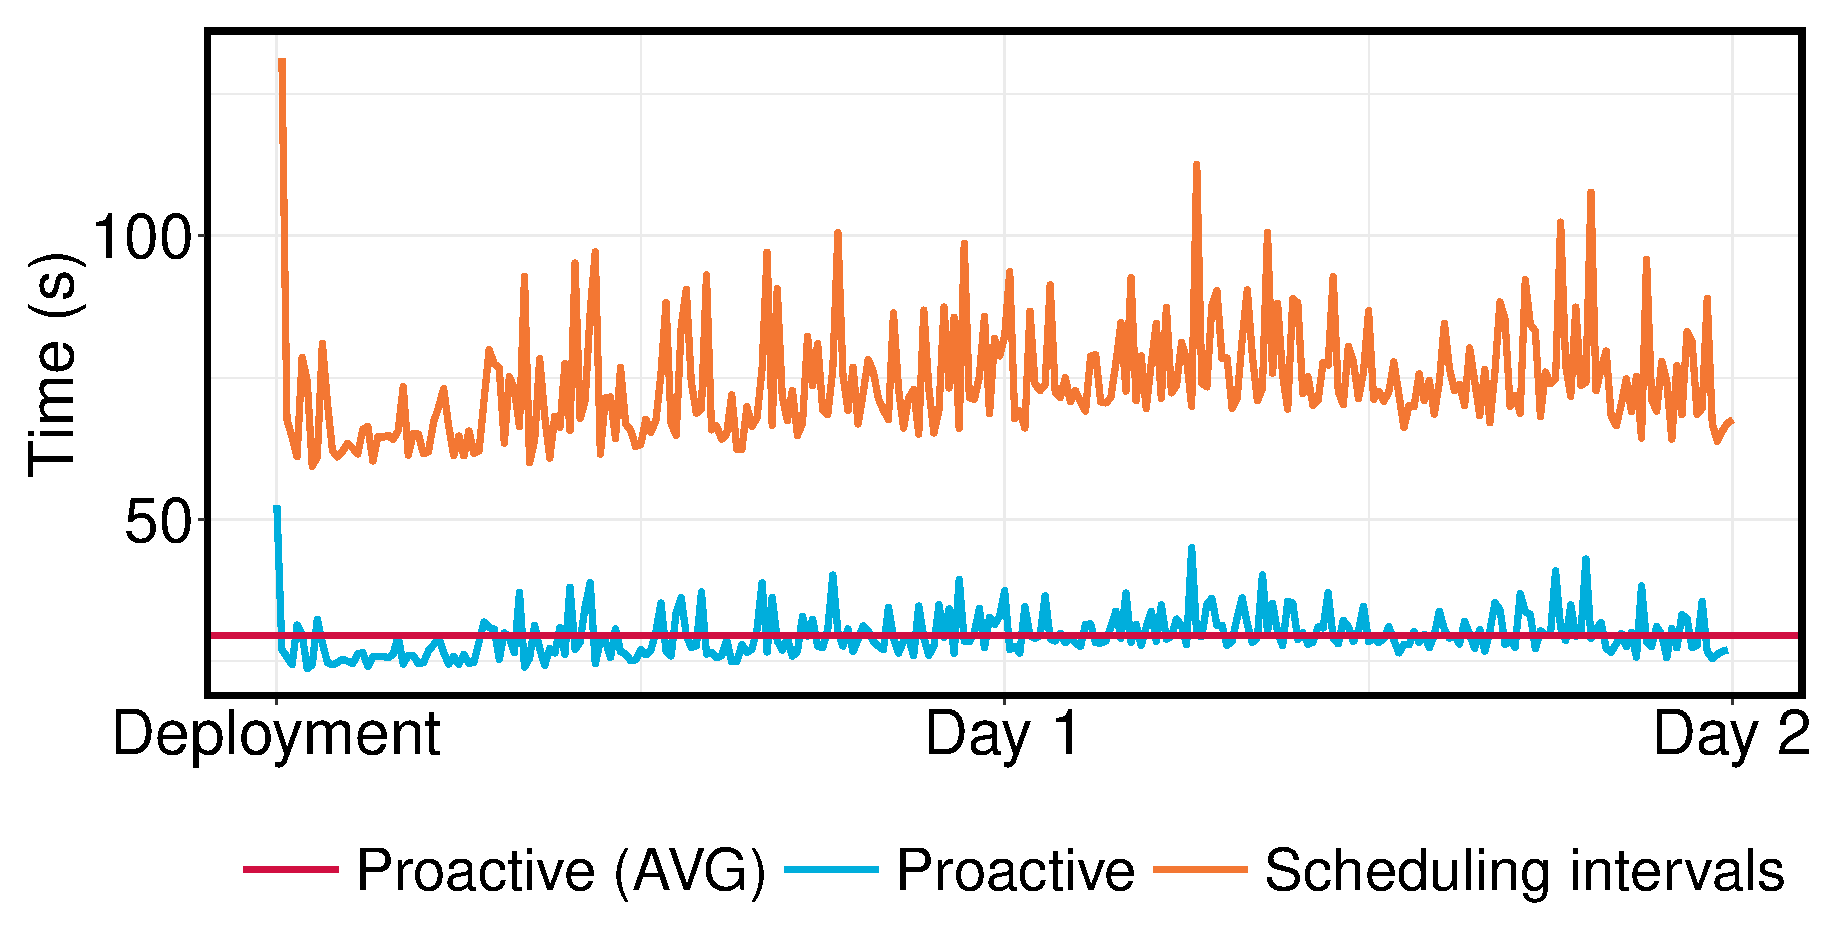
\includegraphics[width=\columnwidth]{../images/experiment-results/criteo-scheduling-experiment.eps}
%\caption{Analysis of scheduling policy}
%\label{fig:scheduling-policy-time}
%\vspace{2mm}
%\end{figure}
%
%Using the slack parameter, we can guide the scheduler to increase or decrease the scheduling intervals of the proactive training.
%The slack parameter allows for the deployment platform to accommodate surges in the incoming prediction requests and new training data.
%In scenarios where sudden surges are expected (e.g., online stores), we recommend a large slack parameter (recommended value is $10$). \todo[inline]{No exp. validate this}

\subsection{EX3: Optimizations Effects}
In this experiment, we analyze the effects of the optimizations, namely, online statistics computation and materialization of features, on the deployment cost (total data preprocessing, and model training time).
Figure \ref{optimization-effect} shows the effect of optimizations on deployment cost.
Online statistics computation and feature materialization eliminate the need for data preprocessing.
As a result, proactive training computes the gradient and updates the deployed model without the need for data preprocessing.
Our optimizations improve the deployment cost by 70\% and 130\% for the URL and Taxi dataset, respectively.
The Taxi pipeline is more complex and contains more components than the URL pipeline.
As a result, the reduction in the Taxi dataset is greater than the URL dataset.

\begin{figure}[h!]
\centering
\resizebox{\columnwidth}{!}{% Created by tikzDevice version 0.11 on 2018-04-23 15:52:24
% !TEX encoding = UTF-8 Unicode
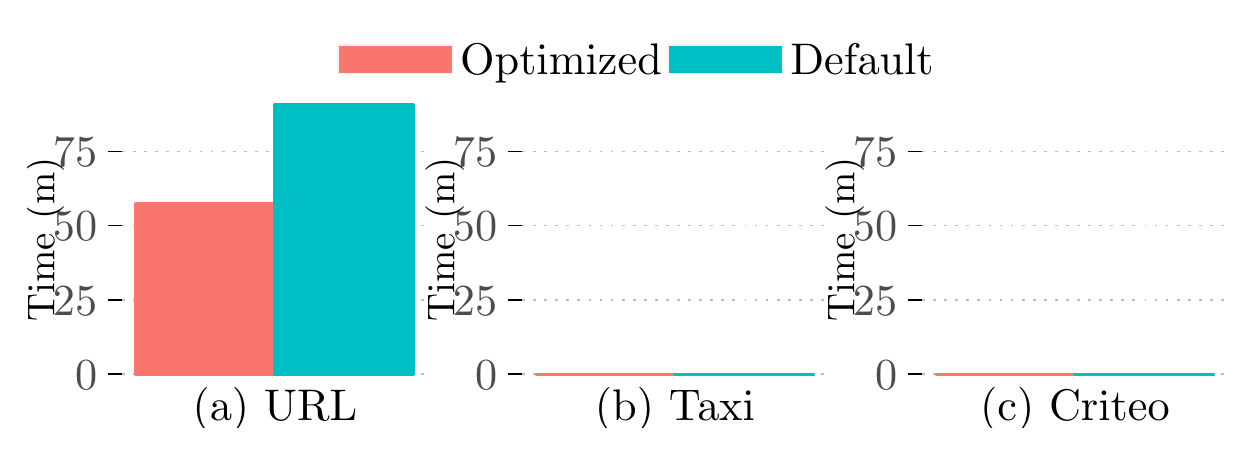
\begin{tikzpicture}[x=1pt,y=1pt]
\definecolor{fillColor}{RGB}{255,255,255}
\path[use as bounding box,fill=fillColor,fill opacity=0.00] (0,0) rectangle (433.62,144.54);
\begin{scope}
\path[clip] (  0.00,  0.00) rectangle (433.62,144.54);
\definecolor{fillColor}{RGB}{255,255,255}

\path[fill=fillColor] (101.43,121.66) rectangle (332.19,144.54);
\end{scope}
\begin{scope}
\path[clip] (  0.00,  0.00) rectangle (433.62,144.54);
\definecolor{drawColor}{RGB}{0,0,0}

\node[text=drawColor,anchor=base west,inner sep=0pt, outer sep=0pt, scale=  0.00] at (107.12,133.10) {Deployment};
\end{scope}
\begin{scope}
\path[clip] (  0.00,  0.00) rectangle (433.62,144.54);
\definecolor{drawColor}{RGB}{255,255,255}
\definecolor{fillColor}{gray}{0.95}

\path[draw=drawColor,line width= 0.6pt,line join=round,line cap=round,fill=fillColor] (111.46,127.35) rectangle (154.14,138.85);
\end{scope}
\begin{scope}
\path[clip] (  0.00,  0.00) rectangle (433.62,144.54);
\definecolor{drawColor}{RGB}{248,118,109}
\definecolor{fillColor}{RGB}{248,118,109}

\path[draw=drawColor,line width= 1.1pt,line cap=round,fill=fillColor] (112.88,128.78) rectangle (152.71,137.43);
\end{scope}
\begin{scope}
\path[clip] (  0.00,  0.00) rectangle (433.62,144.54);
\definecolor{drawColor}{RGB}{255,255,255}
\definecolor{fillColor}{gray}{0.95}

\path[draw=drawColor,line width= 0.6pt,line join=round,line cap=round,fill=fillColor] (230.77,127.35) rectangle (273.45,138.85);
\end{scope}
\begin{scope}
\path[clip] (  0.00,  0.00) rectangle (433.62,144.54);
\definecolor{drawColor}{RGB}{0,191,196}
\definecolor{fillColor}{RGB}{0,191,196}

\path[draw=drawColor,line width= 1.1pt,line cap=round,fill=fillColor] (232.19,128.78) rectangle (272.02,137.43);
\end{scope}
\begin{scope}
\path[clip] (  0.00,  0.00) rectangle (433.62,144.54);
\definecolor{drawColor}{RGB}{0,0,0}

\node[text=drawColor,anchor=base west,inner sep=0pt, outer sep=0pt, scale=  1.60] at (156.30,127.59) {Optimized};
\end{scope}
\begin{scope}
\path[clip] (  0.00,  0.00) rectangle (433.62,144.54);
\definecolor{drawColor}{RGB}{0,0,0}

\node[text=drawColor,anchor=base west,inner sep=0pt, outer sep=0pt, scale=  1.60] at (275.61,127.59) {Default};
\end{scope}
\begin{scope}
\path[clip] (  0.00,  0.00) rectangle (144.54,121.66);
\definecolor{drawColor}{RGB}{255,255,255}
\definecolor{fillColor}{RGB}{255,255,255}

\path[draw=drawColor,line width= 0.6pt,line join=round,line cap=round,fill=fillColor] (  0.00, -0.00) rectangle (144.54,121.66);
\end{scope}
\begin{scope}
\path[clip] ( 34.13, 14.51) rectangle (144.54,121.66);
\definecolor{fillColor}{RGB}{255,255,255}

\path[fill=fillColor] ( 34.13, 14.51) rectangle (144.54,121.66);
\definecolor{drawColor}{RGB}{255,255,255}

\path[draw=drawColor,line width= 0.3pt,line join=round] ( 34.13, 32.79) --
	(144.54, 32.79);

\path[draw=drawColor,line width= 0.3pt,line join=round] ( 34.13, 59.60) --
	(144.54, 59.60);

\path[draw=drawColor,line width= 0.3pt,line join=round] ( 34.13, 86.41) --
	(144.54, 86.41);

\path[draw=drawColor,line width= 0.3pt,line join=round] ( 34.13,113.22) --
	(144.54,113.22);
\definecolor{drawColor}{RGB}{190,190,190}

\path[draw=drawColor,line width= 0.6pt,dash pattern=on 1pt off 3pt ,line join=round] ( 34.13, 19.38) --
	(144.54, 19.38);

\path[draw=drawColor,line width= 0.6pt,dash pattern=on 1pt off 3pt ,line join=round] ( 34.13, 46.19) --
	(144.54, 46.19);

\path[draw=drawColor,line width= 0.6pt,dash pattern=on 1pt off 3pt ,line join=round] ( 34.13, 73.00) --
	(144.54, 73.00);

\path[draw=drawColor,line width= 0.6pt,dash pattern=on 1pt off 3pt ,line join=round] ( 34.13, 99.81) --
	(144.54, 99.81);
\definecolor{drawColor}{RGB}{255,255,255}

\path[draw=drawColor,line width= 0.6pt,line join=round] ( 64.24, 14.51) --
	( 64.24,121.66);

\path[draw=drawColor,line width= 0.6pt,line join=round] (114.43, 14.51) --
	(114.43,121.66);
\definecolor{drawColor}{RGB}{248,118,109}
\definecolor{fillColor}{RGB}{248,118,109}

\path[draw=drawColor,line width= 1.1pt,line join=round,fill=fillColor] ( 39.15, 19.38) rectangle ( 89.34, 80.88);
\definecolor{drawColor}{RGB}{0,191,196}
\definecolor{fillColor}{RGB}{0,191,196}

\path[draw=drawColor,line width= 1.1pt,line join=round,fill=fillColor] ( 89.34, 19.38) rectangle (139.52,116.79);
\end{scope}
\begin{scope}
\path[clip] (  0.00,  0.00) rectangle (433.62,144.54);
\definecolor{drawColor}{gray}{0.30}

\node[text=drawColor,anchor=base east,inner sep=0pt, outer sep=0pt, scale=  1.60] at ( 25.13, 13.87) {0};

\node[text=drawColor,anchor=base east,inner sep=0pt, outer sep=0pt, scale=  1.60] at ( 25.13, 40.68) {25};

\node[text=drawColor,anchor=base east,inner sep=0pt, outer sep=0pt, scale=  1.60] at ( 25.13, 67.49) {50};

\node[text=drawColor,anchor=base east,inner sep=0pt, outer sep=0pt, scale=  1.60] at ( 25.13, 94.30) {75};
\end{scope}
\begin{scope}
\path[clip] (  0.00,  0.00) rectangle (433.62,144.54);
\definecolor{drawColor}{RGB}{0,0,0}

\path[draw=drawColor,line width= 0.6pt,line join=round] ( 29.13, 19.38) --
	( 34.13, 19.38);

\path[draw=drawColor,line width= 0.6pt,line join=round] ( 29.13, 46.19) --
	( 34.13, 46.19);

\path[draw=drawColor,line width= 0.6pt,line join=round] ( 29.13, 73.00) --
	( 34.13, 73.00);

\path[draw=drawColor,line width= 0.6pt,line join=round] ( 29.13, 99.81) --
	( 34.13, 99.81);
\end{scope}
\begin{scope}
\path[clip] (  0.00,  0.00) rectangle (433.62,144.54);
\definecolor{drawColor}{RGB}{0,0,0}

\node[text=drawColor,anchor=base,inner sep=0pt, outer sep=0pt, scale=  1.60] at ( 89.34,  2.49) {(a) URL};
\end{scope}
\begin{scope}
\path[clip] (  0.00,  0.00) rectangle (433.62,144.54);
\definecolor{drawColor}{RGB}{0,0,0}

\node[text=drawColor,rotate= 90.00,anchor=base,inner sep=0pt, outer sep=0pt, scale=  1.40] at (  9.64, 68.09) {Time (m)};
\end{scope}
\begin{scope}
\path[clip] (144.54,  0.00) rectangle (289.08,121.66);
\definecolor{drawColor}{RGB}{255,255,255}
\definecolor{fillColor}{RGB}{255,255,255}

\path[draw=drawColor,line width= 0.6pt,line join=round,line cap=round,fill=fillColor] (144.54, -0.00) rectangle (289.08,121.66);
\end{scope}
\begin{scope}
\path[clip] (178.67, 14.51) rectangle (289.08,121.66);
\definecolor{fillColor}{RGB}{255,255,255}

\path[fill=fillColor] (178.67, 14.51) rectangle (289.08,121.66);
\definecolor{drawColor}{RGB}{255,255,255}

\path[draw=drawColor,line width= 0.3pt,line join=round] (178.67, 32.79) --
	(289.08, 32.79);

\path[draw=drawColor,line width= 0.3pt,line join=round] (178.67, 59.60) --
	(289.08, 59.60);

\path[draw=drawColor,line width= 0.3pt,line join=round] (178.67, 86.41) --
	(289.08, 86.41);

\path[draw=drawColor,line width= 0.3pt,line join=round] (178.67,113.22) --
	(289.08,113.22);
\definecolor{drawColor}{RGB}{190,190,190}

\path[draw=drawColor,line width= 0.6pt,dash pattern=on 1pt off 3pt ,line join=round] (178.67, 19.38) --
	(289.08, 19.38);

\path[draw=drawColor,line width= 0.6pt,dash pattern=on 1pt off 3pt ,line join=round] (178.67, 46.19) --
	(289.08, 46.19);

\path[draw=drawColor,line width= 0.6pt,dash pattern=on 1pt off 3pt ,line join=round] (178.67, 73.00) --
	(289.08, 73.00);

\path[draw=drawColor,line width= 0.6pt,dash pattern=on 1pt off 3pt ,line join=round] (178.67, 99.81) --
	(289.08, 99.81);
\definecolor{drawColor}{RGB}{255,255,255}

\path[draw=drawColor,line width= 0.6pt,line join=round] (208.78, 14.51) --
	(208.78,121.66);

\path[draw=drawColor,line width= 0.6pt,line join=round] (258.97, 14.51) --
	(258.97,121.66);
\definecolor{drawColor}{RGB}{248,118,109}
\definecolor{fillColor}{RGB}{248,118,109}

\path[draw=drawColor,line width= 1.1pt,line join=round,fill=fillColor] (183.69, 19.38) rectangle (233.88, 19.38);
\definecolor{drawColor}{RGB}{0,191,196}
\definecolor{fillColor}{RGB}{0,191,196}

\path[draw=drawColor,line width= 1.1pt,line join=round,fill=fillColor] (233.88, 19.38) rectangle (284.06, 19.38);
\end{scope}
\begin{scope}
\path[clip] (  0.00,  0.00) rectangle (433.62,144.54);
\definecolor{drawColor}{gray}{0.30}

\node[text=drawColor,anchor=base east,inner sep=0pt, outer sep=0pt, scale=  1.60] at (169.67, 13.87) {0};

\node[text=drawColor,anchor=base east,inner sep=0pt, outer sep=0pt, scale=  1.60] at (169.67, 40.68) {25};

\node[text=drawColor,anchor=base east,inner sep=0pt, outer sep=0pt, scale=  1.60] at (169.67, 67.49) {50};

\node[text=drawColor,anchor=base east,inner sep=0pt, outer sep=0pt, scale=  1.60] at (169.67, 94.30) {75};
\end{scope}
\begin{scope}
\path[clip] (  0.00,  0.00) rectangle (433.62,144.54);
\definecolor{drawColor}{RGB}{0,0,0}

\path[draw=drawColor,line width= 0.6pt,line join=round] (173.67, 19.38) --
	(178.67, 19.38);

\path[draw=drawColor,line width= 0.6pt,line join=round] (173.67, 46.19) --
	(178.67, 46.19);

\path[draw=drawColor,line width= 0.6pt,line join=round] (173.67, 73.00) --
	(178.67, 73.00);

\path[draw=drawColor,line width= 0.6pt,line join=round] (173.67, 99.81) --
	(178.67, 99.81);
\end{scope}
\begin{scope}
\path[clip] (  0.00,  0.00) rectangle (433.62,144.54);
\definecolor{drawColor}{RGB}{0,0,0}

\node[text=drawColor,anchor=base,inner sep=0pt, outer sep=0pt, scale=  1.60] at (233.88,  2.49) {(b) Taxi};
\end{scope}
\begin{scope}
\path[clip] (  0.00,  0.00) rectangle (433.62,144.54);
\definecolor{drawColor}{RGB}{0,0,0}

\node[text=drawColor,rotate= 90.00,anchor=base,inner sep=0pt, outer sep=0pt, scale=  1.40] at (154.18, 68.09) {Time (m)};
\end{scope}
\begin{scope}
\path[clip] (289.08,  0.00) rectangle (433.62,121.66);
\definecolor{drawColor}{RGB}{255,255,255}
\definecolor{fillColor}{RGB}{255,255,255}

\path[draw=drawColor,line width= 0.6pt,line join=round,line cap=round,fill=fillColor] (289.08, -0.00) rectangle (433.62,121.66);
\end{scope}
\begin{scope}
\path[clip] (323.21, 14.51) rectangle (433.62,121.66);
\definecolor{fillColor}{RGB}{255,255,255}

\path[fill=fillColor] (323.21, 14.51) rectangle (433.62,121.66);
\definecolor{drawColor}{RGB}{255,255,255}

\path[draw=drawColor,line width= 0.3pt,line join=round] (323.21, 32.79) --
	(433.62, 32.79);

\path[draw=drawColor,line width= 0.3pt,line join=round] (323.21, 59.60) --
	(433.62, 59.60);

\path[draw=drawColor,line width= 0.3pt,line join=round] (323.21, 86.41) --
	(433.62, 86.41);

\path[draw=drawColor,line width= 0.3pt,line join=round] (323.21,113.22) --
	(433.62,113.22);
\definecolor{drawColor}{RGB}{190,190,190}

\path[draw=drawColor,line width= 0.6pt,dash pattern=on 1pt off 3pt ,line join=round] (323.21, 19.38) --
	(433.62, 19.38);

\path[draw=drawColor,line width= 0.6pt,dash pattern=on 1pt off 3pt ,line join=round] (323.21, 46.19) --
	(433.62, 46.19);

\path[draw=drawColor,line width= 0.6pt,dash pattern=on 1pt off 3pt ,line join=round] (323.21, 73.00) --
	(433.62, 73.00);

\path[draw=drawColor,line width= 0.6pt,dash pattern=on 1pt off 3pt ,line join=round] (323.21, 99.81) --
	(433.62, 99.81);
\definecolor{drawColor}{RGB}{255,255,255}

\path[draw=drawColor,line width= 0.6pt,line join=round] (353.32, 14.51) --
	(353.32,121.66);

\path[draw=drawColor,line width= 0.6pt,line join=round] (403.51, 14.51) --
	(403.51,121.66);
\definecolor{drawColor}{RGB}{248,118,109}
\definecolor{fillColor}{RGB}{248,118,109}

\path[draw=drawColor,line width= 1.1pt,line join=round,fill=fillColor] (328.23, 19.38) rectangle (378.42, 19.38);
\definecolor{drawColor}{RGB}{0,191,196}
\definecolor{fillColor}{RGB}{0,191,196}

\path[draw=drawColor,line width= 1.1pt,line join=round,fill=fillColor] (378.42, 19.38) rectangle (428.60, 19.38);
\end{scope}
\begin{scope}
\path[clip] (  0.00,  0.00) rectangle (433.62,144.54);
\definecolor{drawColor}{gray}{0.30}

\node[text=drawColor,anchor=base east,inner sep=0pt, outer sep=0pt, scale=  1.60] at (314.21, 13.87) {0};

\node[text=drawColor,anchor=base east,inner sep=0pt, outer sep=0pt, scale=  1.60] at (314.21, 40.68) {25};

\node[text=drawColor,anchor=base east,inner sep=0pt, outer sep=0pt, scale=  1.60] at (314.21, 67.49) {50};

\node[text=drawColor,anchor=base east,inner sep=0pt, outer sep=0pt, scale=  1.60] at (314.21, 94.30) {75};
\end{scope}
\begin{scope}
\path[clip] (  0.00,  0.00) rectangle (433.62,144.54);
\definecolor{drawColor}{RGB}{0,0,0}

\path[draw=drawColor,line width= 0.6pt,line join=round] (318.21, 19.38) --
	(323.21, 19.38);

\path[draw=drawColor,line width= 0.6pt,line join=round] (318.21, 46.19) --
	(323.21, 46.19);

\path[draw=drawColor,line width= 0.6pt,line join=round] (318.21, 73.00) --
	(323.21, 73.00);

\path[draw=drawColor,line width= 0.6pt,line join=round] (318.21, 99.81) --
	(323.21, 99.81);
\end{scope}
\begin{scope}
\path[clip] (  0.00,  0.00) rectangle (433.62,144.54);
\definecolor{drawColor}{RGB}{0,0,0}

\node[text=drawColor,anchor=base,inner sep=0pt, outer sep=0pt, scale=  1.60] at (378.42,  2.49) {(c) Criteo};
\end{scope}
\begin{scope}
\path[clip] (  0.00,  0.00) rectangle (433.62,144.54);
\definecolor{drawColor}{RGB}{0,0,0}

\node[text=drawColor,rotate= 90.00,anchor=base,inner sep=0pt, outer sep=0pt, scale=  1.40] at (298.72, 68.09) {Time (m)};
\end{scope}
\end{tikzpicture}
}
\caption{Effect of the optimizations on total training time in continuous deployment approach}
\label{optimization-effect}
\end{figure}

\subsection{Discussion} \label{subsec:discussion}
\textbf{Trade off between quality and training cost.}
In many of the real-world use cases, even a small improvement in the quality of a deployed model has an important impact.
Therefore, one can employ more complex pipelines and machine learning models to train better models.
However, during the deployment where prediction queries and training data becomes available at a high rate, one must consider the effect of the training time.
To ensure the model is always up-to-date, the platform must constantly update the model.
Long retraining time has a negative impact on the prediction accuracy as deployed model quickly becomes stale.
Figure \ref{trade-off-figure} shows the trade-off between the quality and total cost of the deployment.

By utilizing continuous deployment, we improve the quality by 0.05\% and 0.3\% for the Taxi and URL datasets over the periodical deployment approach.
We also reduce the cost of the deployment 5 to 13 times when compared with periodical deployment.

\begin{figure}[!h]
\centering
\resizebox{\columnwidth}{!}{% Created by tikzDevice version 0.11 on 2018-04-20 13:31:25
% !TEX encoding = UTF-8 Unicode
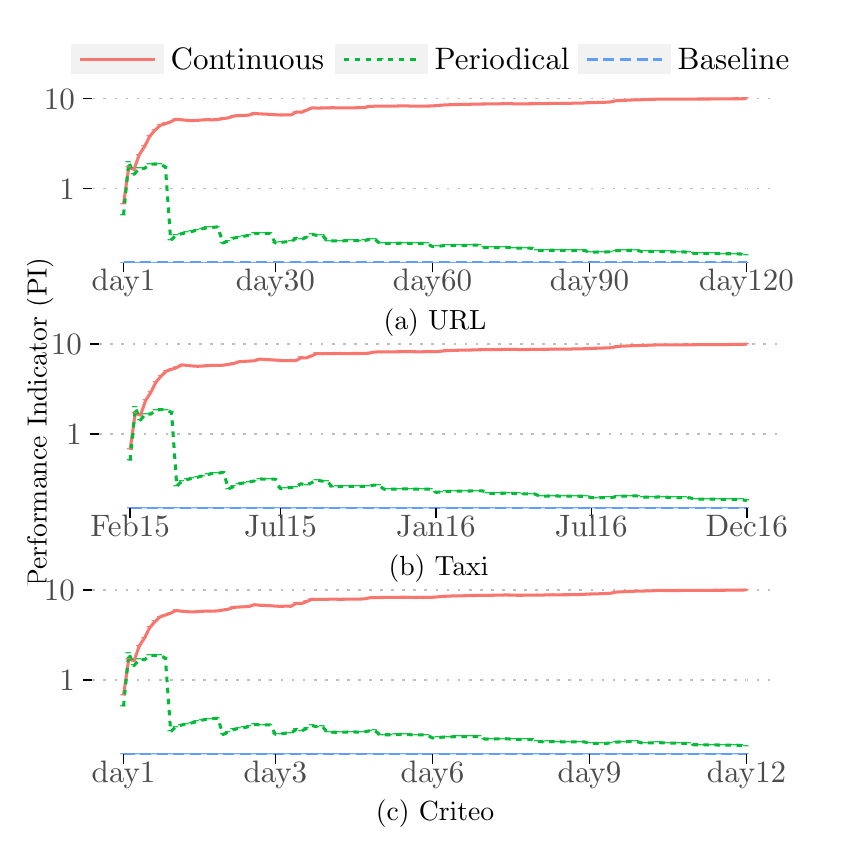
\begin{tikzpicture}[x=1pt,y=1pt]
\definecolor{fillColor}{RGB}{255,255,255}
\path[use as bounding box,fill=fillColor,fill opacity=0.00] (0,0) rectangle (289.08,289.08);
\begin{scope}
\path[clip] (  0.00,  0.00) rectangle (289.08,289.08);
\definecolor{fillColor}{RGB}{255,255,255}

\path[fill=fillColor] (  5.36,266.32) rectangle (283.72,289.08);
\end{scope}
\begin{scope}
\path[clip] (  0.00,  0.00) rectangle (289.08,289.08);
\definecolor{drawColor}{RGB}{255,255,255}
\definecolor{fillColor}{gray}{0.95}

\path[draw=drawColor,line width= 0.6pt,line join=round,line cap=round,fill=fillColor] ( 15.39,272.01) rectangle ( 49.53,283.39);
\end{scope}
\begin{scope}
\path[clip] (  0.00,  0.00) rectangle (289.08,289.08);
\definecolor{drawColor}{RGB}{248,118,109}

\path[draw=drawColor,line width= 1.1pt,line join=round] ( 18.81,277.70) -- ( 46.12,277.70);
\end{scope}
\begin{scope}
\path[clip] (  0.00,  0.00) rectangle (289.08,289.08);
\definecolor{drawColor}{RGB}{248,118,109}

\node[text=drawColor,anchor=base,inner sep=0pt, outer sep=0pt, scale=  0.72] at ( 32.46,276.15) {-};
\end{scope}
\begin{scope}
\path[clip] (  0.00,  0.00) rectangle (289.08,289.08);
\definecolor{drawColor}{RGB}{255,255,255}
\definecolor{fillColor}{gray}{0.95}

\path[draw=drawColor,line width= 0.6pt,line join=round,line cap=round,fill=fillColor] (110.75,272.01) rectangle (144.89,283.39);
\end{scope}
\begin{scope}
\path[clip] (  0.00,  0.00) rectangle (289.08,289.08);
\definecolor{drawColor}{RGB}{0,186,56}

\path[draw=drawColor,line width= 1.1pt,dash pattern=on 2pt off 2pt ,line join=round] (114.16,277.70) -- (141.47,277.70);
\end{scope}
\begin{scope}
\path[clip] (  0.00,  0.00) rectangle (289.08,289.08);
\definecolor{drawColor}{RGB}{0,186,56}

\node[text=drawColor,anchor=base,inner sep=0pt, outer sep=0pt, scale=  0.72] at (127.82,276.15) {-};
\end{scope}
\begin{scope}
\path[clip] (  0.00,  0.00) rectangle (289.08,289.08);
\definecolor{drawColor}{RGB}{255,255,255}
\definecolor{fillColor}{gray}{0.95}

\path[draw=drawColor,line width= 0.6pt,line join=round,line cap=round,fill=fillColor] (198.59,272.01) rectangle (232.73,283.39);
\end{scope}
\begin{scope}
\path[clip] (  0.00,  0.00) rectangle (289.08,289.08);
\definecolor{drawColor}{RGB}{97,156,255}

\path[draw=drawColor,line width= 1.1pt,dash pattern=on 4pt off 2pt ,line join=round] (202.00,277.70) -- (229.32,277.70);
\end{scope}
\begin{scope}
\path[clip] (  0.00,  0.00) rectangle (289.08,289.08);
\definecolor{drawColor}{RGB}{97,156,255}

\node[text=drawColor,anchor=base,inner sep=0pt, outer sep=0pt, scale=  0.72] at (215.66,276.15) {-};
\end{scope}
\begin{scope}
\path[clip] (  0.00,  0.00) rectangle (289.08,289.08);
\definecolor{drawColor}{RGB}{0,0,0}

\node[text=drawColor,anchor=base west,inner sep=0pt, outer sep=0pt, scale=  1.12] at ( 51.70,273.84) {Continuous};
\end{scope}
\begin{scope}
\path[clip] (  0.00,  0.00) rectangle (289.08,289.08);
\definecolor{drawColor}{RGB}{0,0,0}

\node[text=drawColor,anchor=base west,inner sep=0pt, outer sep=0pt, scale=  1.12] at (147.06,273.84) {Periodical};
\end{scope}
\begin{scope}
\path[clip] (  0.00,  0.00) rectangle (289.08,289.08);
\definecolor{drawColor}{RGB}{0,0,0}

\node[text=drawColor,anchor=base west,inner sep=0pt, outer sep=0pt, scale=  1.12] at (234.90,273.84) {Baseline};
\end{scope}
\begin{scope}
\path[clip] (  0.00,177.55) rectangle (289.08,266.32);
\definecolor{drawColor}{RGB}{255,255,255}
\definecolor{fillColor}{RGB}{255,255,255}

\path[draw=drawColor,line width= 0.6pt,line join=round,line cap=round,fill=fillColor] (  0.00,177.55) rectangle (289.08,266.32);
\end{scope}
\begin{scope}
\path[clip] ( 23.38,204.14) rectangle (271.01,266.32);
\definecolor{fillColor}{RGB}{255,255,255}

\path[fill=fillColor] ( 23.38,204.14) rectangle (271.01,266.32);
\definecolor{drawColor}{RGB}{255,255,255}

\path[draw=drawColor,line width= 0.3pt,line join=round] ( 23.38,214.59) --
	(271.01,214.59);

\path[draw=drawColor,line width= 0.3pt,line join=round] ( 23.38,247.22) --
	(271.01,247.22);

\path[draw=drawColor,line width= 0.3pt,line join=round] ( 62.07,204.14) --
	( 62.07,266.32);

\path[draw=drawColor,line width= 0.3pt,line join=round] (117.88,204.14) --
	(117.88,266.32);

\path[draw=drawColor,line width= 0.3pt,line join=round] (174.63,204.14) --
	(174.63,266.32);

\path[draw=drawColor,line width= 0.3pt,line join=round] (231.38,204.14) --
	(231.38,266.32);
\definecolor{drawColor}{RGB}{190,190,190}

\path[draw=drawColor,line width= 0.6pt,dash pattern=on 1pt off 3pt ,line join=round] ( 23.38,230.91) --
	(271.01,230.91);

\path[draw=drawColor,line width= 0.6pt,dash pattern=on 1pt off 3pt ,line join=round] ( 23.38,263.54) --
	(271.01,263.54);
\definecolor{drawColor}{RGB}{255,255,255}

\path[draw=drawColor,line width= 0.6pt,line join=round] ( 34.64,204.14) --
	( 34.64,266.32);

\path[draw=drawColor,line width= 0.6pt,line join=round] ( 89.50,204.14) --
	( 89.50,266.32);

\path[draw=drawColor,line width= 0.6pt,line join=round] (146.25,204.14) --
	(146.25,266.32);

\path[draw=drawColor,line width= 0.6pt,line join=round] (203.00,204.14) --
	(203.00,266.32);

\path[draw=drawColor,line width= 0.6pt,line join=round] (259.76,204.14) --
	(259.76,266.32);
\definecolor{drawColor}{RGB}{248,118,109}

\path[draw=drawColor,line width= 1.1pt,line join=round] ( 34.64,225.42) --
	( 36.53,238.58) --
	( 38.42,237.83) --
	( 40.32,243.17) --
	( 42.21,246.09) --
	( 44.10,249.81) --
	( 45.99,251.99) --
	( 47.88,253.76) --
	( 49.77,254.38) --
	( 51.67,255.05) --
	( 53.56,256.00) --
	( 55.45,255.80) --
	( 57.34,255.62) --
	( 59.23,255.49) --
	( 61.12,255.57) --
	( 63.02,255.72) --
	( 64.91,255.83) --
	( 66.80,255.78) --
	( 68.69,255.89) --
	( 70.58,256.20) --
	( 72.47,256.48) --
	( 74.37,257.14) --
	( 76.26,257.27) --
	( 78.15,257.36) --
	( 80.04,257.49) --
	( 81.93,258.11) --
	( 83.83,257.93) --
	( 85.72,257.85) --
	( 87.61,257.74) --
	( 89.50,257.61) --
	( 91.39,257.51) --
	( 93.28,257.59) --
	( 95.18,257.54) --
	( 97.07,258.61) --
	( 98.96,258.51) --
	(100.85,259.27) --
	(102.74,260.09) --
	(104.63,260.02) --
	(106.53,260.06) --
	(108.42,260.08) --
	(110.31,260.16) --
	(112.20,260.07) --
	(114.09,260.08) --
	(115.98,260.12) --
	(117.88,260.12) --
	(119.77,260.16) --
	(121.66,260.21) --
	(123.55,260.61) --
	(125.44,260.70) --
	(127.34,260.70) --
	(129.23,260.74) --
	(131.12,260.73) --
	(133.01,260.75) --
	(134.90,260.81) --
	(136.79,260.81) --
	(138.69,260.74) --
	(140.58,260.71) --
	(142.47,260.76) --
	(144.36,260.75) --
	(146.25,260.80) --
	(148.14,260.95) --
	(150.04,261.12) --
	(151.93,261.21) --
	(153.82,261.29) --
	(155.71,261.32) --
	(157.60,261.35) --
	(159.49,261.39) --
	(161.39,261.45) --
	(163.28,261.48) --
	(165.17,261.50) --
	(167.06,261.52) --
	(168.95,261.54) --
	(170.85,261.57) --
	(172.74,261.64) --
	(174.63,261.61) --
	(176.52,261.54) --
	(178.41,261.52) --
	(180.30,261.57) --
	(182.20,261.59) --
	(184.09,261.62) --
	(185.98,261.60) --
	(187.87,261.66) --
	(189.76,261.70) --
	(191.65,261.69) --
	(193.55,261.71) --
	(195.44,261.72) --
	(197.33,261.79) --
	(199.22,261.79) --
	(201.11,261.87) --
	(203.00,261.97) --
	(204.90,262.01) --
	(206.79,262.08) --
	(208.68,262.12) --
	(210.57,262.23) --
	(212.46,262.66) --
	(214.36,262.77) --
	(216.25,262.84) --
	(218.14,262.95) --
	(220.03,263.00) --
	(221.92,263.04) --
	(223.81,263.10) --
	(225.71,263.15) --
	(227.60,263.26) --
	(229.49,263.26) --
	(231.38,263.23) --
	(233.27,263.23) --
	(235.16,263.24) --
	(237.06,263.27) --
	(238.95,263.26) --
	(240.84,263.27) --
	(242.73,263.31) --
	(244.62,263.31) --
	(246.51,263.31) --
	(248.41,263.34) --
	(250.30,263.32) --
	(252.19,263.34) --
	(254.08,263.38) --
	(255.97,263.39) --
	(257.86,263.38) --
	(259.76,263.49);
\definecolor{drawColor}{RGB}{0,186,56}

\path[draw=drawColor,line width= 1.1pt,dash pattern=on 2pt off 2pt ,line join=round] ( 34.64,221.39) --
	( 36.53,240.55) --
	( 38.42,236.07) --
	( 40.32,238.33) --
	( 42.21,238.22) --
	( 44.10,239.72) --
	( 45.99,239.82) --
	( 47.88,239.76) --
	( 49.77,238.79) --
	( 51.67,212.22) --
	( 53.56,213.99) --
	( 55.45,214.60) --
	( 57.34,215.00) --
	( 59.23,215.38) --
	( 61.12,215.93) --
	( 63.02,216.39) --
	( 64.91,216.80) --
	( 66.80,216.89) --
	( 68.69,217.13) --
	( 70.58,211.24) --
	( 72.47,212.02) --
	( 74.37,213.03) --
	( 76.26,213.37) --
	( 78.15,213.71) --
	( 80.04,214.06) --
	( 81.93,214.78) --
	( 83.83,214.72) --
	( 85.72,214.72) --
	( 87.61,214.70) --
	( 89.50,211.26) --
	( 91.39,211.46) --
	( 93.28,211.70) --
	( 95.18,211.79) --
	( 97.07,213.06) --
	( 98.96,212.50) --
	(100.85,213.43) --
	(102.74,214.42) --
	(104.63,214.00) --
	(106.53,214.03) --
	(108.42,211.87) --
	(110.31,212.04) --
	(112.20,211.99) --
	(114.09,212.07) --
	(115.98,212.12) --
	(117.88,212.13) --
	(119.77,212.08) --
	(121.66,212.14) --
	(123.55,212.55) --
	(125.44,212.62) --
	(127.34,211.06) --
	(129.23,211.13) --
	(131.12,211.11) --
	(133.01,211.15) --
	(134.90,211.20) --
	(136.79,211.20) --
	(138.69,211.12) --
	(140.58,211.06) --
	(142.47,211.10) --
	(144.36,211.07) --
	(146.25,209.95) --
	(148.14,210.09) --
	(150.04,210.28) --
	(151.93,210.34) --
	(153.82,210.40) --
	(155.71,210.41) --
	(157.60,210.42) --
	(159.49,210.44) --
	(161.39,210.48) --
	(163.28,210.50) --
	(165.17,209.57) --
	(167.06,209.59) --
	(168.95,209.60) --
	(170.85,209.63) --
	(172.74,209.68) --
	(174.63,209.55) --
	(176.52,209.46) --
	(178.41,209.40) --
	(180.30,209.40) --
	(182.20,209.37) --
	(184.09,208.65) --
	(185.98,208.60) --
	(187.87,208.63) --
	(189.76,208.65) --
	(191.65,208.59) --
	(193.55,208.58) --
	(195.44,208.55) --
	(197.33,208.57) --
	(199.22,208.52) --
	(201.11,208.56) --
	(203.00,208.02) --
	(204.90,208.00) --
	(206.79,208.02) --
	(208.68,208.02) --
	(210.57,208.10) --
	(212.46,208.47) --
	(214.36,208.54) --
	(216.25,208.58) --
	(218.14,208.65) --
	(220.03,208.66) --
	(221.92,208.17) --
	(223.81,208.20) --
	(225.71,208.20) --
	(227.60,208.28) --
	(229.49,208.22) --
	(231.38,208.14) --
	(233.27,208.09) --
	(235.16,208.06) --
	(237.06,208.03) --
	(238.95,207.97) --
	(240.84,207.52) --
	(242.73,207.51) --
	(244.62,207.49) --
	(246.51,207.46) --
	(248.41,207.45) --
	(250.30,207.40) --
	(252.19,207.38) --
	(254.08,207.39) --
	(255.97,207.34) --
	(257.86,207.28) --
	(259.76,206.97);
\definecolor{drawColor}{RGB}{97,156,255}

\path[draw=drawColor,line width= 1.1pt,dash pattern=on 4pt off 2pt ,line join=round] ( 34.64,204.14) --
	( 36.53,204.14) --
	( 38.42,204.14) --
	( 40.32,204.14) --
	( 42.21,204.14) --
	( 44.10,204.14) --
	( 45.99,204.14) --
	( 47.88,204.14) --
	( 49.77,204.14) --
	( 51.67,204.14) --
	( 53.56,204.14) --
	( 55.45,204.14) --
	( 57.34,204.14) --
	( 59.23,204.14) --
	( 61.12,204.14) --
	( 63.02,204.14) --
	( 64.91,204.14) --
	( 66.80,204.14) --
	( 68.69,204.14) --
	( 70.58,204.14) --
	( 72.47,204.14) --
	( 74.37,204.14) --
	( 76.26,204.14) --
	( 78.15,204.14) --
	( 80.04,204.14) --
	( 81.93,204.14) --
	( 83.83,204.14) --
	( 85.72,204.14) --
	( 87.61,204.14) --
	( 89.50,204.14) --
	( 91.39,204.14) --
	( 93.28,204.14) --
	( 95.18,204.14) --
	( 97.07,204.14) --
	( 98.96,204.14) --
	(100.85,204.14) --
	(102.74,204.14) --
	(104.63,204.14) --
	(106.53,204.14) --
	(108.42,204.14) --
	(110.31,204.14) --
	(112.20,204.14) --
	(114.09,204.14) --
	(115.98,204.14) --
	(117.88,204.14) --
	(119.77,204.14) --
	(121.66,204.14) --
	(123.55,204.14) --
	(125.44,204.14) --
	(127.34,204.14) --
	(129.23,204.14) --
	(131.12,204.14) --
	(133.01,204.14) --
	(134.90,204.14) --
	(136.79,204.14) --
	(138.69,204.14) --
	(140.58,204.14) --
	(142.47,204.14) --
	(144.36,204.14) --
	(146.25,204.14) --
	(148.14,204.14) --
	(150.04,204.14) --
	(151.93,204.14) --
	(153.82,204.14) --
	(155.71,204.14) --
	(157.60,204.14) --
	(159.49,204.14) --
	(161.39,204.14) --
	(163.28,204.14) --
	(165.17,204.14) --
	(167.06,204.14) --
	(168.95,204.14) --
	(170.85,204.14) --
	(172.74,204.14) --
	(174.63,204.14) --
	(176.52,204.14) --
	(178.41,204.14) --
	(180.30,204.14) --
	(182.20,204.14) --
	(184.09,204.14) --
	(185.98,204.14) --
	(187.87,204.14) --
	(189.76,204.14) --
	(191.65,204.14) --
	(193.55,204.14) --
	(195.44,204.14) --
	(197.33,204.14) --
	(199.22,204.14) --
	(201.11,204.14) --
	(203.00,204.14) --
	(204.90,204.14) --
	(206.79,204.14) --
	(208.68,204.14) --
	(210.57,204.14) --
	(212.46,204.14) --
	(214.36,204.14) --
	(216.25,204.14) --
	(218.14,204.14) --
	(220.03,204.14) --
	(221.92,204.14) --
	(223.81,204.14) --
	(225.71,204.14) --
	(227.60,204.14) --
	(229.49,204.14) --
	(231.38,204.14) --
	(233.27,204.14) --
	(235.16,204.14) --
	(237.06,204.14) --
	(238.95,204.14) --
	(240.84,204.14) --
	(242.73,204.14) --
	(244.62,204.14) --
	(246.51,204.14) --
	(248.41,204.14) --
	(250.30,204.14) --
	(252.19,204.14) --
	(254.08,204.14) --
	(255.97,204.14) --
	(257.86,204.14) --
	(259.76,204.14);
\definecolor{drawColor}{RGB}{248,118,109}

\node[text=drawColor,anchor=base,inner sep=0pt, outer sep=0pt, scale=  0.72] at ( 34.64,223.87) {-};

\node[text=drawColor,anchor=base,inner sep=0pt, outer sep=0pt, scale=  0.72] at ( 36.53,237.03) {-};

\node[text=drawColor,anchor=base,inner sep=0pt, outer sep=0pt, scale=  0.72] at ( 38.42,236.28) {-};

\node[text=drawColor,anchor=base,inner sep=0pt, outer sep=0pt, scale=  0.72] at ( 40.32,241.62) {-};

\node[text=drawColor,anchor=base,inner sep=0pt, outer sep=0pt, scale=  0.72] at ( 42.21,244.54) {-};

\node[text=drawColor,anchor=base,inner sep=0pt, outer sep=0pt, scale=  0.72] at ( 44.10,248.26) {-};

\node[text=drawColor,anchor=base,inner sep=0pt, outer sep=0pt, scale=  0.72] at ( 45.99,250.44) {-};

\node[text=drawColor,anchor=base,inner sep=0pt, outer sep=0pt, scale=  0.72] at ( 47.88,252.21) {-};

\node[text=drawColor,anchor=base,inner sep=0pt, outer sep=0pt, scale=  0.72] at ( 49.77,252.83) {-};

\node[text=drawColor,anchor=base,inner sep=0pt, outer sep=0pt, scale=  0.72] at ( 51.67,253.49) {-};

\node[text=drawColor,anchor=base,inner sep=0pt, outer sep=0pt, scale=  0.72] at ( 53.56,254.45) {-};

\node[text=drawColor,anchor=base,inner sep=0pt, outer sep=0pt, scale=  0.72] at ( 55.45,254.25) {-};

\node[text=drawColor,anchor=base,inner sep=0pt, outer sep=0pt, scale=  0.72] at ( 57.34,254.07) {-};

\node[text=drawColor,anchor=base,inner sep=0pt, outer sep=0pt, scale=  0.72] at ( 59.23,253.94) {-};

\node[text=drawColor,anchor=base,inner sep=0pt, outer sep=0pt, scale=  0.72] at ( 61.12,254.02) {-};

\node[text=drawColor,anchor=base,inner sep=0pt, outer sep=0pt, scale=  0.72] at ( 63.02,254.17) {-};

\node[text=drawColor,anchor=base,inner sep=0pt, outer sep=0pt, scale=  0.72] at ( 64.91,254.28) {-};

\node[text=drawColor,anchor=base,inner sep=0pt, outer sep=0pt, scale=  0.72] at ( 66.80,254.23) {-};

\node[text=drawColor,anchor=base,inner sep=0pt, outer sep=0pt, scale=  0.72] at ( 68.69,254.34) {-};

\node[text=drawColor,anchor=base,inner sep=0pt, outer sep=0pt, scale=  0.72] at ( 70.58,254.65) {-};

\node[text=drawColor,anchor=base,inner sep=0pt, outer sep=0pt, scale=  0.72] at ( 72.47,254.93) {-};

\node[text=drawColor,anchor=base,inner sep=0pt, outer sep=0pt, scale=  0.72] at ( 74.37,255.59) {-};

\node[text=drawColor,anchor=base,inner sep=0pt, outer sep=0pt, scale=  0.72] at ( 76.26,255.72) {-};

\node[text=drawColor,anchor=base,inner sep=0pt, outer sep=0pt, scale=  0.72] at ( 78.15,255.81) {-};

\node[text=drawColor,anchor=base,inner sep=0pt, outer sep=0pt, scale=  0.72] at ( 80.04,255.94) {-};

\node[text=drawColor,anchor=base,inner sep=0pt, outer sep=0pt, scale=  0.72] at ( 81.93,256.56) {-};

\node[text=drawColor,anchor=base,inner sep=0pt, outer sep=0pt, scale=  0.72] at ( 83.83,256.38) {-};

\node[text=drawColor,anchor=base,inner sep=0pt, outer sep=0pt, scale=  0.72] at ( 85.72,256.30) {-};

\node[text=drawColor,anchor=base,inner sep=0pt, outer sep=0pt, scale=  0.72] at ( 87.61,256.19) {-};

\node[text=drawColor,anchor=base,inner sep=0pt, outer sep=0pt, scale=  0.72] at ( 89.50,256.05) {-};

\node[text=drawColor,anchor=base,inner sep=0pt, outer sep=0pt, scale=  0.72] at ( 91.39,255.96) {-};

\node[text=drawColor,anchor=base,inner sep=0pt, outer sep=0pt, scale=  0.72] at ( 93.28,256.04) {-};

\node[text=drawColor,anchor=base,inner sep=0pt, outer sep=0pt, scale=  0.72] at ( 95.18,255.99) {-};

\node[text=drawColor,anchor=base,inner sep=0pt, outer sep=0pt, scale=  0.72] at ( 97.07,257.06) {-};

\node[text=drawColor,anchor=base,inner sep=0pt, outer sep=0pt, scale=  0.72] at ( 98.96,256.96) {-};

\node[text=drawColor,anchor=base,inner sep=0pt, outer sep=0pt, scale=  0.72] at (100.85,257.72) {-};

\node[text=drawColor,anchor=base,inner sep=0pt, outer sep=0pt, scale=  0.72] at (102.74,258.54) {-};

\node[text=drawColor,anchor=base,inner sep=0pt, outer sep=0pt, scale=  0.72] at (104.63,258.47) {-};

\node[text=drawColor,anchor=base,inner sep=0pt, outer sep=0pt, scale=  0.72] at (106.53,258.51) {-};

\node[text=drawColor,anchor=base,inner sep=0pt, outer sep=0pt, scale=  0.72] at (108.42,258.53) {-};

\node[text=drawColor,anchor=base,inner sep=0pt, outer sep=0pt, scale=  0.72] at (110.31,258.61) {-};

\node[text=drawColor,anchor=base,inner sep=0pt, outer sep=0pt, scale=  0.72] at (112.20,258.52) {-};

\node[text=drawColor,anchor=base,inner sep=0pt, outer sep=0pt, scale=  0.72] at (114.09,258.53) {-};

\node[text=drawColor,anchor=base,inner sep=0pt, outer sep=0pt, scale=  0.72] at (115.98,258.57) {-};

\node[text=drawColor,anchor=base,inner sep=0pt, outer sep=0pt, scale=  0.72] at (117.88,258.57) {-};

\node[text=drawColor,anchor=base,inner sep=0pt, outer sep=0pt, scale=  0.72] at (119.77,258.61) {-};

\node[text=drawColor,anchor=base,inner sep=0pt, outer sep=0pt, scale=  0.72] at (121.66,258.66) {-};

\node[text=drawColor,anchor=base,inner sep=0pt, outer sep=0pt, scale=  0.72] at (123.55,259.06) {-};

\node[text=drawColor,anchor=base,inner sep=0pt, outer sep=0pt, scale=  0.72] at (125.44,259.15) {-};

\node[text=drawColor,anchor=base,inner sep=0pt, outer sep=0pt, scale=  0.72] at (127.34,259.15) {-};

\node[text=drawColor,anchor=base,inner sep=0pt, outer sep=0pt, scale=  0.72] at (129.23,259.18) {-};

\node[text=drawColor,anchor=base,inner sep=0pt, outer sep=0pt, scale=  0.72] at (131.12,259.18) {-};

\node[text=drawColor,anchor=base,inner sep=0pt, outer sep=0pt, scale=  0.72] at (133.01,259.20) {-};

\node[text=drawColor,anchor=base,inner sep=0pt, outer sep=0pt, scale=  0.72] at (134.90,259.26) {-};

\node[text=drawColor,anchor=base,inner sep=0pt, outer sep=0pt, scale=  0.72] at (136.79,259.26) {-};

\node[text=drawColor,anchor=base,inner sep=0pt, outer sep=0pt, scale=  0.72] at (138.69,259.19) {-};

\node[text=drawColor,anchor=base,inner sep=0pt, outer sep=0pt, scale=  0.72] at (140.58,259.16) {-};

\node[text=drawColor,anchor=base,inner sep=0pt, outer sep=0pt, scale=  0.72] at (142.47,259.21) {-};

\node[text=drawColor,anchor=base,inner sep=0pt, outer sep=0pt, scale=  0.72] at (144.36,259.20) {-};

\node[text=drawColor,anchor=base,inner sep=0pt, outer sep=0pt, scale=  0.72] at (146.25,259.25) {-};

\node[text=drawColor,anchor=base,inner sep=0pt, outer sep=0pt, scale=  0.72] at (148.14,259.40) {-};

\node[text=drawColor,anchor=base,inner sep=0pt, outer sep=0pt, scale=  0.72] at (150.04,259.57) {-};

\node[text=drawColor,anchor=base,inner sep=0pt, outer sep=0pt, scale=  0.72] at (151.93,259.66) {-};

\node[text=drawColor,anchor=base,inner sep=0pt, outer sep=0pt, scale=  0.72] at (153.82,259.73) {-};

\node[text=drawColor,anchor=base,inner sep=0pt, outer sep=0pt, scale=  0.72] at (155.71,259.77) {-};

\node[text=drawColor,anchor=base,inner sep=0pt, outer sep=0pt, scale=  0.72] at (157.60,259.80) {-};

\node[text=drawColor,anchor=base,inner sep=0pt, outer sep=0pt, scale=  0.72] at (159.49,259.84) {-};

\node[text=drawColor,anchor=base,inner sep=0pt, outer sep=0pt, scale=  0.72] at (161.39,259.90) {-};

\node[text=drawColor,anchor=base,inner sep=0pt, outer sep=0pt, scale=  0.72] at (163.28,259.93) {-};

\node[text=drawColor,anchor=base,inner sep=0pt, outer sep=0pt, scale=  0.72] at (165.17,259.95) {-};

\node[text=drawColor,anchor=base,inner sep=0pt, outer sep=0pt, scale=  0.72] at (167.06,259.97) {-};

\node[text=drawColor,anchor=base,inner sep=0pt, outer sep=0pt, scale=  0.72] at (168.95,259.99) {-};

\node[text=drawColor,anchor=base,inner sep=0pt, outer sep=0pt, scale=  0.72] at (170.85,260.02) {-};

\node[text=drawColor,anchor=base,inner sep=0pt, outer sep=0pt, scale=  0.72] at (172.74,260.09) {-};

\node[text=drawColor,anchor=base,inner sep=0pt, outer sep=0pt, scale=  0.72] at (174.63,260.06) {-};

\node[text=drawColor,anchor=base,inner sep=0pt, outer sep=0pt, scale=  0.72] at (176.52,259.99) {-};

\node[text=drawColor,anchor=base,inner sep=0pt, outer sep=0pt, scale=  0.72] at (178.41,259.97) {-};

\node[text=drawColor,anchor=base,inner sep=0pt, outer sep=0pt, scale=  0.72] at (180.30,260.02) {-};

\node[text=drawColor,anchor=base,inner sep=0pt, outer sep=0pt, scale=  0.72] at (182.20,260.04) {-};

\node[text=drawColor,anchor=base,inner sep=0pt, outer sep=0pt, scale=  0.72] at (184.09,260.07) {-};

\node[text=drawColor,anchor=base,inner sep=0pt, outer sep=0pt, scale=  0.72] at (185.98,260.05) {-};

\node[text=drawColor,anchor=base,inner sep=0pt, outer sep=0pt, scale=  0.72] at (187.87,260.11) {-};

\node[text=drawColor,anchor=base,inner sep=0pt, outer sep=0pt, scale=  0.72] at (189.76,260.15) {-};

\node[text=drawColor,anchor=base,inner sep=0pt, outer sep=0pt, scale=  0.72] at (191.65,260.14) {-};

\node[text=drawColor,anchor=base,inner sep=0pt, outer sep=0pt, scale=  0.72] at (193.55,260.16) {-};

\node[text=drawColor,anchor=base,inner sep=0pt, outer sep=0pt, scale=  0.72] at (195.44,260.17) {-};

\node[text=drawColor,anchor=base,inner sep=0pt, outer sep=0pt, scale=  0.72] at (197.33,260.24) {-};

\node[text=drawColor,anchor=base,inner sep=0pt, outer sep=0pt, scale=  0.72] at (199.22,260.24) {-};

\node[text=drawColor,anchor=base,inner sep=0pt, outer sep=0pt, scale=  0.72] at (201.11,260.32) {-};

\node[text=drawColor,anchor=base,inner sep=0pt, outer sep=0pt, scale=  0.72] at (203.00,260.42) {-};

\node[text=drawColor,anchor=base,inner sep=0pt, outer sep=0pt, scale=  0.72] at (204.90,260.46) {-};

\node[text=drawColor,anchor=base,inner sep=0pt, outer sep=0pt, scale=  0.72] at (206.79,260.53) {-};

\node[text=drawColor,anchor=base,inner sep=0pt, outer sep=0pt, scale=  0.72] at (208.68,260.57) {-};

\node[text=drawColor,anchor=base,inner sep=0pt, outer sep=0pt, scale=  0.72] at (210.57,260.68) {-};

\node[text=drawColor,anchor=base,inner sep=0pt, outer sep=0pt, scale=  0.72] at (212.46,261.11) {-};

\node[text=drawColor,anchor=base,inner sep=0pt, outer sep=0pt, scale=  0.72] at (214.36,261.22) {-};

\node[text=drawColor,anchor=base,inner sep=0pt, outer sep=0pt, scale=  0.72] at (216.25,261.29) {-};

\node[text=drawColor,anchor=base,inner sep=0pt, outer sep=0pt, scale=  0.72] at (218.14,261.40) {-};

\node[text=drawColor,anchor=base,inner sep=0pt, outer sep=0pt, scale=  0.72] at (220.03,261.45) {-};

\node[text=drawColor,anchor=base,inner sep=0pt, outer sep=0pt, scale=  0.72] at (221.92,261.49) {-};

\node[text=drawColor,anchor=base,inner sep=0pt, outer sep=0pt, scale=  0.72] at (223.81,261.55) {-};

\node[text=drawColor,anchor=base,inner sep=0pt, outer sep=0pt, scale=  0.72] at (225.71,261.60) {-};

\node[text=drawColor,anchor=base,inner sep=0pt, outer sep=0pt, scale=  0.72] at (227.60,261.71) {-};

\node[text=drawColor,anchor=base,inner sep=0pt, outer sep=0pt, scale=  0.72] at (229.49,261.71) {-};

\node[text=drawColor,anchor=base,inner sep=0pt, outer sep=0pt, scale=  0.72] at (231.38,261.68) {-};

\node[text=drawColor,anchor=base,inner sep=0pt, outer sep=0pt, scale=  0.72] at (233.27,261.68) {-};

\node[text=drawColor,anchor=base,inner sep=0pt, outer sep=0pt, scale=  0.72] at (235.16,261.69) {-};

\node[text=drawColor,anchor=base,inner sep=0pt, outer sep=0pt, scale=  0.72] at (237.06,261.72) {-};

\node[text=drawColor,anchor=base,inner sep=0pt, outer sep=0pt, scale=  0.72] at (238.95,261.71) {-};

\node[text=drawColor,anchor=base,inner sep=0pt, outer sep=0pt, scale=  0.72] at (240.84,261.72) {-};

\node[text=drawColor,anchor=base,inner sep=0pt, outer sep=0pt, scale=  0.72] at (242.73,261.76) {-};

\node[text=drawColor,anchor=base,inner sep=0pt, outer sep=0pt, scale=  0.72] at (244.62,261.76) {-};

\node[text=drawColor,anchor=base,inner sep=0pt, outer sep=0pt, scale=  0.72] at (246.51,261.76) {-};

\node[text=drawColor,anchor=base,inner sep=0pt, outer sep=0pt, scale=  0.72] at (248.41,261.78) {-};

\node[text=drawColor,anchor=base,inner sep=0pt, outer sep=0pt, scale=  0.72] at (250.30,261.77) {-};

\node[text=drawColor,anchor=base,inner sep=0pt, outer sep=0pt, scale=  0.72] at (252.19,261.79) {-};

\node[text=drawColor,anchor=base,inner sep=0pt, outer sep=0pt, scale=  0.72] at (254.08,261.83) {-};

\node[text=drawColor,anchor=base,inner sep=0pt, outer sep=0pt, scale=  0.72] at (255.97,261.84) {-};

\node[text=drawColor,anchor=base,inner sep=0pt, outer sep=0pt, scale=  0.72] at (257.86,261.83) {-};

\node[text=drawColor,anchor=base,inner sep=0pt, outer sep=0pt, scale=  0.72] at (259.76,261.94) {-};
\definecolor{drawColor}{RGB}{0,186,56}

\node[text=drawColor,anchor=base,inner sep=0pt, outer sep=0pt, scale=  0.72] at ( 34.64,219.84) {-};

\node[text=drawColor,anchor=base,inner sep=0pt, outer sep=0pt, scale=  0.72] at ( 36.53,239.00) {-};

\node[text=drawColor,anchor=base,inner sep=0pt, outer sep=0pt, scale=  0.72] at ( 38.42,234.52) {-};

\node[text=drawColor,anchor=base,inner sep=0pt, outer sep=0pt, scale=  0.72] at ( 40.32,236.78) {-};

\node[text=drawColor,anchor=base,inner sep=0pt, outer sep=0pt, scale=  0.72] at ( 42.21,236.67) {-};

\node[text=drawColor,anchor=base,inner sep=0pt, outer sep=0pt, scale=  0.72] at ( 44.10,238.17) {-};

\node[text=drawColor,anchor=base,inner sep=0pt, outer sep=0pt, scale=  0.72] at ( 45.99,238.27) {-};

\node[text=drawColor,anchor=base,inner sep=0pt, outer sep=0pt, scale=  0.72] at ( 47.88,238.21) {-};

\node[text=drawColor,anchor=base,inner sep=0pt, outer sep=0pt, scale=  0.72] at ( 49.77,237.24) {-};

\node[text=drawColor,anchor=base,inner sep=0pt, outer sep=0pt, scale=  0.72] at ( 51.67,210.67) {-};

\node[text=drawColor,anchor=base,inner sep=0pt, outer sep=0pt, scale=  0.72] at ( 53.56,212.43) {-};

\node[text=drawColor,anchor=base,inner sep=0pt, outer sep=0pt, scale=  0.72] at ( 55.45,213.05) {-};

\node[text=drawColor,anchor=base,inner sep=0pt, outer sep=0pt, scale=  0.72] at ( 57.34,213.45) {-};

\node[text=drawColor,anchor=base,inner sep=0pt, outer sep=0pt, scale=  0.72] at ( 59.23,213.83) {-};

\node[text=drawColor,anchor=base,inner sep=0pt, outer sep=0pt, scale=  0.72] at ( 61.12,214.38) {-};

\node[text=drawColor,anchor=base,inner sep=0pt, outer sep=0pt, scale=  0.72] at ( 63.02,214.84) {-};

\node[text=drawColor,anchor=base,inner sep=0pt, outer sep=0pt, scale=  0.72] at ( 64.91,215.25) {-};

\node[text=drawColor,anchor=base,inner sep=0pt, outer sep=0pt, scale=  0.72] at ( 66.80,215.34) {-};

\node[text=drawColor,anchor=base,inner sep=0pt, outer sep=0pt, scale=  0.72] at ( 68.69,215.58) {-};

\node[text=drawColor,anchor=base,inner sep=0pt, outer sep=0pt, scale=  0.72] at ( 70.58,209.69) {-};

\node[text=drawColor,anchor=base,inner sep=0pt, outer sep=0pt, scale=  0.72] at ( 72.47,210.47) {-};

\node[text=drawColor,anchor=base,inner sep=0pt, outer sep=0pt, scale=  0.72] at ( 74.37,211.48) {-};

\node[text=drawColor,anchor=base,inner sep=0pt, outer sep=0pt, scale=  0.72] at ( 76.26,211.82) {-};

\node[text=drawColor,anchor=base,inner sep=0pt, outer sep=0pt, scale=  0.72] at ( 78.15,212.16) {-};

\node[text=drawColor,anchor=base,inner sep=0pt, outer sep=0pt, scale=  0.72] at ( 80.04,212.51) {-};

\node[text=drawColor,anchor=base,inner sep=0pt, outer sep=0pt, scale=  0.72] at ( 81.93,213.23) {-};

\node[text=drawColor,anchor=base,inner sep=0pt, outer sep=0pt, scale=  0.72] at ( 83.83,213.17) {-};

\node[text=drawColor,anchor=base,inner sep=0pt, outer sep=0pt, scale=  0.72] at ( 85.72,213.17) {-};

\node[text=drawColor,anchor=base,inner sep=0pt, outer sep=0pt, scale=  0.72] at ( 87.61,213.15) {-};

\node[text=drawColor,anchor=base,inner sep=0pt, outer sep=0pt, scale=  0.72] at ( 89.50,209.71) {-};

\node[text=drawColor,anchor=base,inner sep=0pt, outer sep=0pt, scale=  0.72] at ( 91.39,209.91) {-};

\node[text=drawColor,anchor=base,inner sep=0pt, outer sep=0pt, scale=  0.72] at ( 93.28,210.15) {-};

\node[text=drawColor,anchor=base,inner sep=0pt, outer sep=0pt, scale=  0.72] at ( 95.18,210.24) {-};

\node[text=drawColor,anchor=base,inner sep=0pt, outer sep=0pt, scale=  0.72] at ( 97.07,211.51) {-};

\node[text=drawColor,anchor=base,inner sep=0pt, outer sep=0pt, scale=  0.72] at ( 98.96,210.95) {-};

\node[text=drawColor,anchor=base,inner sep=0pt, outer sep=0pt, scale=  0.72] at (100.85,211.88) {-};

\node[text=drawColor,anchor=base,inner sep=0pt, outer sep=0pt, scale=  0.72] at (102.74,212.87) {-};

\node[text=drawColor,anchor=base,inner sep=0pt, outer sep=0pt, scale=  0.72] at (104.63,212.45) {-};

\node[text=drawColor,anchor=base,inner sep=0pt, outer sep=0pt, scale=  0.72] at (106.53,212.48) {-};

\node[text=drawColor,anchor=base,inner sep=0pt, outer sep=0pt, scale=  0.72] at (108.42,210.32) {-};

\node[text=drawColor,anchor=base,inner sep=0pt, outer sep=0pt, scale=  0.72] at (110.31,210.49) {-};

\node[text=drawColor,anchor=base,inner sep=0pt, outer sep=0pt, scale=  0.72] at (112.20,210.44) {-};

\node[text=drawColor,anchor=base,inner sep=0pt, outer sep=0pt, scale=  0.72] at (114.09,210.52) {-};

\node[text=drawColor,anchor=base,inner sep=0pt, outer sep=0pt, scale=  0.72] at (115.98,210.57) {-};

\node[text=drawColor,anchor=base,inner sep=0pt, outer sep=0pt, scale=  0.72] at (117.88,210.58) {-};

\node[text=drawColor,anchor=base,inner sep=0pt, outer sep=0pt, scale=  0.72] at (119.77,210.53) {-};

\node[text=drawColor,anchor=base,inner sep=0pt, outer sep=0pt, scale=  0.72] at (121.66,210.59) {-};

\node[text=drawColor,anchor=base,inner sep=0pt, outer sep=0pt, scale=  0.72] at (123.55,211.00) {-};

\node[text=drawColor,anchor=base,inner sep=0pt, outer sep=0pt, scale=  0.72] at (125.44,211.07) {-};

\node[text=drawColor,anchor=base,inner sep=0pt, outer sep=0pt, scale=  0.72] at (127.34,209.50) {-};

\node[text=drawColor,anchor=base,inner sep=0pt, outer sep=0pt, scale=  0.72] at (129.23,209.57) {-};

\node[text=drawColor,anchor=base,inner sep=0pt, outer sep=0pt, scale=  0.72] at (131.12,209.56) {-};

\node[text=drawColor,anchor=base,inner sep=0pt, outer sep=0pt, scale=  0.72] at (133.01,209.60) {-};

\node[text=drawColor,anchor=base,inner sep=0pt, outer sep=0pt, scale=  0.72] at (134.90,209.65) {-};

\node[text=drawColor,anchor=base,inner sep=0pt, outer sep=0pt, scale=  0.72] at (136.79,209.65) {-};

\node[text=drawColor,anchor=base,inner sep=0pt, outer sep=0pt, scale=  0.72] at (138.69,209.57) {-};

\node[text=drawColor,anchor=base,inner sep=0pt, outer sep=0pt, scale=  0.72] at (140.58,209.51) {-};

\node[text=drawColor,anchor=base,inner sep=0pt, outer sep=0pt, scale=  0.72] at (142.47,209.55) {-};

\node[text=drawColor,anchor=base,inner sep=0pt, outer sep=0pt, scale=  0.72] at (144.36,209.52) {-};

\node[text=drawColor,anchor=base,inner sep=0pt, outer sep=0pt, scale=  0.72] at (146.25,208.39) {-};

\node[text=drawColor,anchor=base,inner sep=0pt, outer sep=0pt, scale=  0.72] at (148.14,208.54) {-};

\node[text=drawColor,anchor=base,inner sep=0pt, outer sep=0pt, scale=  0.72] at (150.04,208.73) {-};

\node[text=drawColor,anchor=base,inner sep=0pt, outer sep=0pt, scale=  0.72] at (151.93,208.79) {-};

\node[text=drawColor,anchor=base,inner sep=0pt, outer sep=0pt, scale=  0.72] at (153.82,208.85) {-};

\node[text=drawColor,anchor=base,inner sep=0pt, outer sep=0pt, scale=  0.72] at (155.71,208.86) {-};

\node[text=drawColor,anchor=base,inner sep=0pt, outer sep=0pt, scale=  0.72] at (157.60,208.87) {-};

\node[text=drawColor,anchor=base,inner sep=0pt, outer sep=0pt, scale=  0.72] at (159.49,208.89) {-};

\node[text=drawColor,anchor=base,inner sep=0pt, outer sep=0pt, scale=  0.72] at (161.39,208.93) {-};

\node[text=drawColor,anchor=base,inner sep=0pt, outer sep=0pt, scale=  0.72] at (163.28,208.95) {-};

\node[text=drawColor,anchor=base,inner sep=0pt, outer sep=0pt, scale=  0.72] at (165.17,208.02) {-};

\node[text=drawColor,anchor=base,inner sep=0pt, outer sep=0pt, scale=  0.72] at (167.06,208.04) {-};

\node[text=drawColor,anchor=base,inner sep=0pt, outer sep=0pt, scale=  0.72] at (168.95,208.05) {-};

\node[text=drawColor,anchor=base,inner sep=0pt, outer sep=0pt, scale=  0.72] at (170.85,208.08) {-};

\node[text=drawColor,anchor=base,inner sep=0pt, outer sep=0pt, scale=  0.72] at (172.74,208.13) {-};

\node[text=drawColor,anchor=base,inner sep=0pt, outer sep=0pt, scale=  0.72] at (174.63,208.00) {-};

\node[text=drawColor,anchor=base,inner sep=0pt, outer sep=0pt, scale=  0.72] at (176.52,207.91) {-};

\node[text=drawColor,anchor=base,inner sep=0pt, outer sep=0pt, scale=  0.72] at (178.41,207.85) {-};

\node[text=drawColor,anchor=base,inner sep=0pt, outer sep=0pt, scale=  0.72] at (180.30,207.85) {-};

\node[text=drawColor,anchor=base,inner sep=0pt, outer sep=0pt, scale=  0.72] at (182.20,207.82) {-};

\node[text=drawColor,anchor=base,inner sep=0pt, outer sep=0pt, scale=  0.72] at (184.09,207.10) {-};

\node[text=drawColor,anchor=base,inner sep=0pt, outer sep=0pt, scale=  0.72] at (185.98,207.05) {-};

\node[text=drawColor,anchor=base,inner sep=0pt, outer sep=0pt, scale=  0.72] at (187.87,207.08) {-};

\node[text=drawColor,anchor=base,inner sep=0pt, outer sep=0pt, scale=  0.72] at (189.76,207.10) {-};

\node[text=drawColor,anchor=base,inner sep=0pt, outer sep=0pt, scale=  0.72] at (191.65,207.04) {-};

\node[text=drawColor,anchor=base,inner sep=0pt, outer sep=0pt, scale=  0.72] at (193.55,207.03) {-};

\node[text=drawColor,anchor=base,inner sep=0pt, outer sep=0pt, scale=  0.72] at (195.44,207.00) {-};

\node[text=drawColor,anchor=base,inner sep=0pt, outer sep=0pt, scale=  0.72] at (197.33,207.02) {-};

\node[text=drawColor,anchor=base,inner sep=0pt, outer sep=0pt, scale=  0.72] at (199.22,206.97) {-};

\node[text=drawColor,anchor=base,inner sep=0pt, outer sep=0pt, scale=  0.72] at (201.11,207.01) {-};

\node[text=drawColor,anchor=base,inner sep=0pt, outer sep=0pt, scale=  0.72] at (203.00,206.47) {-};

\node[text=drawColor,anchor=base,inner sep=0pt, outer sep=0pt, scale=  0.72] at (204.90,206.45) {-};

\node[text=drawColor,anchor=base,inner sep=0pt, outer sep=0pt, scale=  0.72] at (206.79,206.47) {-};

\node[text=drawColor,anchor=base,inner sep=0pt, outer sep=0pt, scale=  0.72] at (208.68,206.47) {-};

\node[text=drawColor,anchor=base,inner sep=0pt, outer sep=0pt, scale=  0.72] at (210.57,206.55) {-};

\node[text=drawColor,anchor=base,inner sep=0pt, outer sep=0pt, scale=  0.72] at (212.46,206.92) {-};

\node[text=drawColor,anchor=base,inner sep=0pt, outer sep=0pt, scale=  0.72] at (214.36,206.99) {-};

\node[text=drawColor,anchor=base,inner sep=0pt, outer sep=0pt, scale=  0.72] at (216.25,207.03) {-};

\node[text=drawColor,anchor=base,inner sep=0pt, outer sep=0pt, scale=  0.72] at (218.14,207.10) {-};

\node[text=drawColor,anchor=base,inner sep=0pt, outer sep=0pt, scale=  0.72] at (220.03,207.11) {-};

\node[text=drawColor,anchor=base,inner sep=0pt, outer sep=0pt, scale=  0.72] at (221.92,206.62) {-};

\node[text=drawColor,anchor=base,inner sep=0pt, outer sep=0pt, scale=  0.72] at (223.81,206.65) {-};

\node[text=drawColor,anchor=base,inner sep=0pt, outer sep=0pt, scale=  0.72] at (225.71,206.65) {-};

\node[text=drawColor,anchor=base,inner sep=0pt, outer sep=0pt, scale=  0.72] at (227.60,206.73) {-};

\node[text=drawColor,anchor=base,inner sep=0pt, outer sep=0pt, scale=  0.72] at (229.49,206.67) {-};

\node[text=drawColor,anchor=base,inner sep=0pt, outer sep=0pt, scale=  0.72] at (231.38,206.59) {-};

\node[text=drawColor,anchor=base,inner sep=0pt, outer sep=0pt, scale=  0.72] at (233.27,206.54) {-};

\node[text=drawColor,anchor=base,inner sep=0pt, outer sep=0pt, scale=  0.72] at (235.16,206.51) {-};

\node[text=drawColor,anchor=base,inner sep=0pt, outer sep=0pt, scale=  0.72] at (237.06,206.48) {-};

\node[text=drawColor,anchor=base,inner sep=0pt, outer sep=0pt, scale=  0.72] at (238.95,206.42) {-};

\node[text=drawColor,anchor=base,inner sep=0pt, outer sep=0pt, scale=  0.72] at (240.84,205.96) {-};

\node[text=drawColor,anchor=base,inner sep=0pt, outer sep=0pt, scale=  0.72] at (242.73,205.96) {-};

\node[text=drawColor,anchor=base,inner sep=0pt, outer sep=0pt, scale=  0.72] at (244.62,205.94) {-};

\node[text=drawColor,anchor=base,inner sep=0pt, outer sep=0pt, scale=  0.72] at (246.51,205.91) {-};

\node[text=drawColor,anchor=base,inner sep=0pt, outer sep=0pt, scale=  0.72] at (248.41,205.90) {-};

\node[text=drawColor,anchor=base,inner sep=0pt, outer sep=0pt, scale=  0.72] at (250.30,205.85) {-};

\node[text=drawColor,anchor=base,inner sep=0pt, outer sep=0pt, scale=  0.72] at (252.19,205.83) {-};

\node[text=drawColor,anchor=base,inner sep=0pt, outer sep=0pt, scale=  0.72] at (254.08,205.84) {-};

\node[text=drawColor,anchor=base,inner sep=0pt, outer sep=0pt, scale=  0.72] at (255.97,205.79) {-};

\node[text=drawColor,anchor=base,inner sep=0pt, outer sep=0pt, scale=  0.72] at (257.86,205.73) {-};

\node[text=drawColor,anchor=base,inner sep=0pt, outer sep=0pt, scale=  0.72] at (259.76,205.42) {-};
\definecolor{drawColor}{RGB}{97,156,255}

\node[text=drawColor,anchor=base,inner sep=0pt, outer sep=0pt, scale=  0.72] at ( 34.64,202.59) {-};

\node[text=drawColor,anchor=base,inner sep=0pt, outer sep=0pt, scale=  0.72] at ( 36.53,202.59) {-};

\node[text=drawColor,anchor=base,inner sep=0pt, outer sep=0pt, scale=  0.72] at ( 38.42,202.59) {-};

\node[text=drawColor,anchor=base,inner sep=0pt, outer sep=0pt, scale=  0.72] at ( 40.32,202.59) {-};

\node[text=drawColor,anchor=base,inner sep=0pt, outer sep=0pt, scale=  0.72] at ( 42.21,202.59) {-};

\node[text=drawColor,anchor=base,inner sep=0pt, outer sep=0pt, scale=  0.72] at ( 44.10,202.59) {-};

\node[text=drawColor,anchor=base,inner sep=0pt, outer sep=0pt, scale=  0.72] at ( 45.99,202.59) {-};

\node[text=drawColor,anchor=base,inner sep=0pt, outer sep=0pt, scale=  0.72] at ( 47.88,202.59) {-};

\node[text=drawColor,anchor=base,inner sep=0pt, outer sep=0pt, scale=  0.72] at ( 49.77,202.59) {-};

\node[text=drawColor,anchor=base,inner sep=0pt, outer sep=0pt, scale=  0.72] at ( 51.67,202.59) {-};

\node[text=drawColor,anchor=base,inner sep=0pt, outer sep=0pt, scale=  0.72] at ( 53.56,202.59) {-};

\node[text=drawColor,anchor=base,inner sep=0pt, outer sep=0pt, scale=  0.72] at ( 55.45,202.59) {-};

\node[text=drawColor,anchor=base,inner sep=0pt, outer sep=0pt, scale=  0.72] at ( 57.34,202.59) {-};

\node[text=drawColor,anchor=base,inner sep=0pt, outer sep=0pt, scale=  0.72] at ( 59.23,202.59) {-};

\node[text=drawColor,anchor=base,inner sep=0pt, outer sep=0pt, scale=  0.72] at ( 61.12,202.59) {-};

\node[text=drawColor,anchor=base,inner sep=0pt, outer sep=0pt, scale=  0.72] at ( 63.02,202.59) {-};

\node[text=drawColor,anchor=base,inner sep=0pt, outer sep=0pt, scale=  0.72] at ( 64.91,202.59) {-};

\node[text=drawColor,anchor=base,inner sep=0pt, outer sep=0pt, scale=  0.72] at ( 66.80,202.59) {-};

\node[text=drawColor,anchor=base,inner sep=0pt, outer sep=0pt, scale=  0.72] at ( 68.69,202.59) {-};

\node[text=drawColor,anchor=base,inner sep=0pt, outer sep=0pt, scale=  0.72] at ( 70.58,202.59) {-};

\node[text=drawColor,anchor=base,inner sep=0pt, outer sep=0pt, scale=  0.72] at ( 72.47,202.59) {-};

\node[text=drawColor,anchor=base,inner sep=0pt, outer sep=0pt, scale=  0.72] at ( 74.37,202.59) {-};

\node[text=drawColor,anchor=base,inner sep=0pt, outer sep=0pt, scale=  0.72] at ( 76.26,202.59) {-};

\node[text=drawColor,anchor=base,inner sep=0pt, outer sep=0pt, scale=  0.72] at ( 78.15,202.59) {-};

\node[text=drawColor,anchor=base,inner sep=0pt, outer sep=0pt, scale=  0.72] at ( 80.04,202.59) {-};

\node[text=drawColor,anchor=base,inner sep=0pt, outer sep=0pt, scale=  0.72] at ( 81.93,202.59) {-};

\node[text=drawColor,anchor=base,inner sep=0pt, outer sep=0pt, scale=  0.72] at ( 83.83,202.59) {-};

\node[text=drawColor,anchor=base,inner sep=0pt, outer sep=0pt, scale=  0.72] at ( 85.72,202.59) {-};

\node[text=drawColor,anchor=base,inner sep=0pt, outer sep=0pt, scale=  0.72] at ( 87.61,202.59) {-};

\node[text=drawColor,anchor=base,inner sep=0pt, outer sep=0pt, scale=  0.72] at ( 89.50,202.59) {-};

\node[text=drawColor,anchor=base,inner sep=0pt, outer sep=0pt, scale=  0.72] at ( 91.39,202.59) {-};

\node[text=drawColor,anchor=base,inner sep=0pt, outer sep=0pt, scale=  0.72] at ( 93.28,202.59) {-};

\node[text=drawColor,anchor=base,inner sep=0pt, outer sep=0pt, scale=  0.72] at ( 95.18,202.59) {-};

\node[text=drawColor,anchor=base,inner sep=0pt, outer sep=0pt, scale=  0.72] at ( 97.07,202.59) {-};

\node[text=drawColor,anchor=base,inner sep=0pt, outer sep=0pt, scale=  0.72] at ( 98.96,202.59) {-};

\node[text=drawColor,anchor=base,inner sep=0pt, outer sep=0pt, scale=  0.72] at (100.85,202.59) {-};

\node[text=drawColor,anchor=base,inner sep=0pt, outer sep=0pt, scale=  0.72] at (102.74,202.59) {-};

\node[text=drawColor,anchor=base,inner sep=0pt, outer sep=0pt, scale=  0.72] at (104.63,202.59) {-};

\node[text=drawColor,anchor=base,inner sep=0pt, outer sep=0pt, scale=  0.72] at (106.53,202.59) {-};

\node[text=drawColor,anchor=base,inner sep=0pt, outer sep=0pt, scale=  0.72] at (108.42,202.59) {-};

\node[text=drawColor,anchor=base,inner sep=0pt, outer sep=0pt, scale=  0.72] at (110.31,202.59) {-};

\node[text=drawColor,anchor=base,inner sep=0pt, outer sep=0pt, scale=  0.72] at (112.20,202.59) {-};

\node[text=drawColor,anchor=base,inner sep=0pt, outer sep=0pt, scale=  0.72] at (114.09,202.59) {-};

\node[text=drawColor,anchor=base,inner sep=0pt, outer sep=0pt, scale=  0.72] at (115.98,202.59) {-};

\node[text=drawColor,anchor=base,inner sep=0pt, outer sep=0pt, scale=  0.72] at (117.88,202.59) {-};

\node[text=drawColor,anchor=base,inner sep=0pt, outer sep=0pt, scale=  0.72] at (119.77,202.59) {-};

\node[text=drawColor,anchor=base,inner sep=0pt, outer sep=0pt, scale=  0.72] at (121.66,202.59) {-};

\node[text=drawColor,anchor=base,inner sep=0pt, outer sep=0pt, scale=  0.72] at (123.55,202.59) {-};

\node[text=drawColor,anchor=base,inner sep=0pt, outer sep=0pt, scale=  0.72] at (125.44,202.59) {-};

\node[text=drawColor,anchor=base,inner sep=0pt, outer sep=0pt, scale=  0.72] at (127.34,202.59) {-};

\node[text=drawColor,anchor=base,inner sep=0pt, outer sep=0pt, scale=  0.72] at (129.23,202.59) {-};

\node[text=drawColor,anchor=base,inner sep=0pt, outer sep=0pt, scale=  0.72] at (131.12,202.59) {-};

\node[text=drawColor,anchor=base,inner sep=0pt, outer sep=0pt, scale=  0.72] at (133.01,202.59) {-};

\node[text=drawColor,anchor=base,inner sep=0pt, outer sep=0pt, scale=  0.72] at (134.90,202.59) {-};

\node[text=drawColor,anchor=base,inner sep=0pt, outer sep=0pt, scale=  0.72] at (136.79,202.59) {-};

\node[text=drawColor,anchor=base,inner sep=0pt, outer sep=0pt, scale=  0.72] at (138.69,202.59) {-};

\node[text=drawColor,anchor=base,inner sep=0pt, outer sep=0pt, scale=  0.72] at (140.58,202.59) {-};

\node[text=drawColor,anchor=base,inner sep=0pt, outer sep=0pt, scale=  0.72] at (142.47,202.59) {-};

\node[text=drawColor,anchor=base,inner sep=0pt, outer sep=0pt, scale=  0.72] at (144.36,202.59) {-};

\node[text=drawColor,anchor=base,inner sep=0pt, outer sep=0pt, scale=  0.72] at (146.25,202.59) {-};

\node[text=drawColor,anchor=base,inner sep=0pt, outer sep=0pt, scale=  0.72] at (148.14,202.59) {-};

\node[text=drawColor,anchor=base,inner sep=0pt, outer sep=0pt, scale=  0.72] at (150.04,202.59) {-};

\node[text=drawColor,anchor=base,inner sep=0pt, outer sep=0pt, scale=  0.72] at (151.93,202.59) {-};

\node[text=drawColor,anchor=base,inner sep=0pt, outer sep=0pt, scale=  0.72] at (153.82,202.59) {-};

\node[text=drawColor,anchor=base,inner sep=0pt, outer sep=0pt, scale=  0.72] at (155.71,202.59) {-};

\node[text=drawColor,anchor=base,inner sep=0pt, outer sep=0pt, scale=  0.72] at (157.60,202.59) {-};

\node[text=drawColor,anchor=base,inner sep=0pt, outer sep=0pt, scale=  0.72] at (159.49,202.59) {-};

\node[text=drawColor,anchor=base,inner sep=0pt, outer sep=0pt, scale=  0.72] at (161.39,202.59) {-};

\node[text=drawColor,anchor=base,inner sep=0pt, outer sep=0pt, scale=  0.72] at (163.28,202.59) {-};

\node[text=drawColor,anchor=base,inner sep=0pt, outer sep=0pt, scale=  0.72] at (165.17,202.59) {-};

\node[text=drawColor,anchor=base,inner sep=0pt, outer sep=0pt, scale=  0.72] at (167.06,202.59) {-};

\node[text=drawColor,anchor=base,inner sep=0pt, outer sep=0pt, scale=  0.72] at (168.95,202.59) {-};

\node[text=drawColor,anchor=base,inner sep=0pt, outer sep=0pt, scale=  0.72] at (170.85,202.59) {-};

\node[text=drawColor,anchor=base,inner sep=0pt, outer sep=0pt, scale=  0.72] at (172.74,202.59) {-};

\node[text=drawColor,anchor=base,inner sep=0pt, outer sep=0pt, scale=  0.72] at (174.63,202.59) {-};

\node[text=drawColor,anchor=base,inner sep=0pt, outer sep=0pt, scale=  0.72] at (176.52,202.59) {-};

\node[text=drawColor,anchor=base,inner sep=0pt, outer sep=0pt, scale=  0.72] at (178.41,202.59) {-};

\node[text=drawColor,anchor=base,inner sep=0pt, outer sep=0pt, scale=  0.72] at (180.30,202.59) {-};

\node[text=drawColor,anchor=base,inner sep=0pt, outer sep=0pt, scale=  0.72] at (182.20,202.59) {-};

\node[text=drawColor,anchor=base,inner sep=0pt, outer sep=0pt, scale=  0.72] at (184.09,202.59) {-};

\node[text=drawColor,anchor=base,inner sep=0pt, outer sep=0pt, scale=  0.72] at (185.98,202.59) {-};

\node[text=drawColor,anchor=base,inner sep=0pt, outer sep=0pt, scale=  0.72] at (187.87,202.59) {-};

\node[text=drawColor,anchor=base,inner sep=0pt, outer sep=0pt, scale=  0.72] at (189.76,202.59) {-};

\node[text=drawColor,anchor=base,inner sep=0pt, outer sep=0pt, scale=  0.72] at (191.65,202.59) {-};

\node[text=drawColor,anchor=base,inner sep=0pt, outer sep=0pt, scale=  0.72] at (193.55,202.59) {-};

\node[text=drawColor,anchor=base,inner sep=0pt, outer sep=0pt, scale=  0.72] at (195.44,202.59) {-};

\node[text=drawColor,anchor=base,inner sep=0pt, outer sep=0pt, scale=  0.72] at (197.33,202.59) {-};

\node[text=drawColor,anchor=base,inner sep=0pt, outer sep=0pt, scale=  0.72] at (199.22,202.59) {-};

\node[text=drawColor,anchor=base,inner sep=0pt, outer sep=0pt, scale=  0.72] at (201.11,202.59) {-};

\node[text=drawColor,anchor=base,inner sep=0pt, outer sep=0pt, scale=  0.72] at (203.00,202.59) {-};

\node[text=drawColor,anchor=base,inner sep=0pt, outer sep=0pt, scale=  0.72] at (204.90,202.59) {-};

\node[text=drawColor,anchor=base,inner sep=0pt, outer sep=0pt, scale=  0.72] at (206.79,202.59) {-};

\node[text=drawColor,anchor=base,inner sep=0pt, outer sep=0pt, scale=  0.72] at (208.68,202.59) {-};

\node[text=drawColor,anchor=base,inner sep=0pt, outer sep=0pt, scale=  0.72] at (210.57,202.59) {-};

\node[text=drawColor,anchor=base,inner sep=0pt, outer sep=0pt, scale=  0.72] at (212.46,202.59) {-};

\node[text=drawColor,anchor=base,inner sep=0pt, outer sep=0pt, scale=  0.72] at (214.36,202.59) {-};

\node[text=drawColor,anchor=base,inner sep=0pt, outer sep=0pt, scale=  0.72] at (216.25,202.59) {-};

\node[text=drawColor,anchor=base,inner sep=0pt, outer sep=0pt, scale=  0.72] at (218.14,202.59) {-};

\node[text=drawColor,anchor=base,inner sep=0pt, outer sep=0pt, scale=  0.72] at (220.03,202.59) {-};

\node[text=drawColor,anchor=base,inner sep=0pt, outer sep=0pt, scale=  0.72] at (221.92,202.59) {-};

\node[text=drawColor,anchor=base,inner sep=0pt, outer sep=0pt, scale=  0.72] at (223.81,202.59) {-};

\node[text=drawColor,anchor=base,inner sep=0pt, outer sep=0pt, scale=  0.72] at (225.71,202.59) {-};

\node[text=drawColor,anchor=base,inner sep=0pt, outer sep=0pt, scale=  0.72] at (227.60,202.59) {-};

\node[text=drawColor,anchor=base,inner sep=0pt, outer sep=0pt, scale=  0.72] at (229.49,202.59) {-};

\node[text=drawColor,anchor=base,inner sep=0pt, outer sep=0pt, scale=  0.72] at (231.38,202.59) {-};

\node[text=drawColor,anchor=base,inner sep=0pt, outer sep=0pt, scale=  0.72] at (233.27,202.59) {-};

\node[text=drawColor,anchor=base,inner sep=0pt, outer sep=0pt, scale=  0.72] at (235.16,202.59) {-};

\node[text=drawColor,anchor=base,inner sep=0pt, outer sep=0pt, scale=  0.72] at (237.06,202.59) {-};

\node[text=drawColor,anchor=base,inner sep=0pt, outer sep=0pt, scale=  0.72] at (238.95,202.59) {-};

\node[text=drawColor,anchor=base,inner sep=0pt, outer sep=0pt, scale=  0.72] at (240.84,202.59) {-};

\node[text=drawColor,anchor=base,inner sep=0pt, outer sep=0pt, scale=  0.72] at (242.73,202.59) {-};

\node[text=drawColor,anchor=base,inner sep=0pt, outer sep=0pt, scale=  0.72] at (244.62,202.59) {-};

\node[text=drawColor,anchor=base,inner sep=0pt, outer sep=0pt, scale=  0.72] at (246.51,202.59) {-};

\node[text=drawColor,anchor=base,inner sep=0pt, outer sep=0pt, scale=  0.72] at (248.41,202.59) {-};

\node[text=drawColor,anchor=base,inner sep=0pt, outer sep=0pt, scale=  0.72] at (250.30,202.59) {-};

\node[text=drawColor,anchor=base,inner sep=0pt, outer sep=0pt, scale=  0.72] at (252.19,202.59) {-};

\node[text=drawColor,anchor=base,inner sep=0pt, outer sep=0pt, scale=  0.72] at (254.08,202.59) {-};

\node[text=drawColor,anchor=base,inner sep=0pt, outer sep=0pt, scale=  0.72] at (255.97,202.59) {-};

\node[text=drawColor,anchor=base,inner sep=0pt, outer sep=0pt, scale=  0.72] at (257.86,202.59) {-};

\node[text=drawColor,anchor=base,inner sep=0pt, outer sep=0pt, scale=  0.72] at (259.76,202.59) {-};
\end{scope}
\begin{scope}
\path[clip] (  0.00,  0.00) rectangle (289.08,289.08);
\definecolor{drawColor}{gray}{0.30}

\node[text=drawColor,anchor=base east,inner sep=0pt, outer sep=0pt, scale=  1.12] at ( 17.08,227.05) {1};

\node[text=drawColor,anchor=base east,inner sep=0pt, outer sep=0pt, scale=  1.12] at ( 17.08,259.68) {10};
\end{scope}
\begin{scope}
\path[clip] (  0.00,  0.00) rectangle (289.08,289.08);
\definecolor{drawColor}{RGB}{0,0,0}

\path[draw=drawColor,line width= 0.6pt,line join=round] ( 19.88,230.91) --
	( 23.38,230.91);

\path[draw=drawColor,line width= 0.6pt,line join=round] ( 19.88,263.54) --
	( 23.38,263.54);
\end{scope}
\begin{scope}
\path[clip] (  0.00,  0.00) rectangle (289.08,289.08);
\definecolor{drawColor}{RGB}{0,0,0}

\path[draw=drawColor,line width= 0.6pt,line join=round] ( 34.64,200.64) --
	( 34.64,204.14);

\path[draw=drawColor,line width= 0.6pt,line join=round] ( 89.50,200.64) --
	( 89.50,204.14);

\path[draw=drawColor,line width= 0.6pt,line join=round] (146.25,200.64) --
	(146.25,204.14);

\path[draw=drawColor,line width= 0.6pt,line join=round] (203.00,200.64) --
	(203.00,204.14);

\path[draw=drawColor,line width= 0.6pt,line join=round] (259.76,200.64) --
	(259.76,204.14);
\end{scope}
\begin{scope}
\path[clip] (  0.00,  0.00) rectangle (289.08,289.08);
\definecolor{drawColor}{gray}{0.30}

\node[text=drawColor,anchor=base,inner sep=0pt, outer sep=0pt, scale=  1.12] at ( 34.64,193.93) {day1};

\node[text=drawColor,anchor=base,inner sep=0pt, outer sep=0pt, scale=  1.12] at ( 89.50,193.93) {day30};

\node[text=drawColor,anchor=base,inner sep=0pt, outer sep=0pt, scale=  1.12] at (146.25,193.93) {day60};

\node[text=drawColor,anchor=base,inner sep=0pt, outer sep=0pt, scale=  1.12] at (203.00,193.93) {day90};

\node[text=drawColor,anchor=base,inner sep=0pt, outer sep=0pt, scale=  1.12] at (259.76,193.93) {day120};
\end{scope}
\begin{scope}
\path[clip] (  0.00,  0.00) rectangle (289.08,289.08);
\definecolor{drawColor}{RGB}{0,0,0}

\node[text=drawColor,anchor=base,inner sep=0pt, outer sep=0pt, scale=  1.00] at (147.20,180.04) {(a) URL};
\end{scope}
\begin{scope}
\path[clip] (  0.00, 88.77) rectangle (289.08,177.55);
\definecolor{drawColor}{RGB}{255,255,255}
\definecolor{fillColor}{RGB}{255,255,255}

\path[draw=drawColor,line width= 0.6pt,line join=round,line cap=round,fill=fillColor] ( -0.00, 88.77) rectangle (289.08,177.55);
\end{scope}
\begin{scope}
\path[clip] ( 25.88,115.37) rectangle (271.01,177.55);
\definecolor{fillColor}{RGB}{255,255,255}

\path[fill=fillColor] ( 25.88,115.37) rectangle (271.01,177.55);
\definecolor{drawColor}{RGB}{255,255,255}

\path[draw=drawColor,line width= 0.3pt,line join=round] ( 25.88,125.82) --
	(271.01,125.82);

\path[draw=drawColor,line width= 0.3pt,line join=round] ( 25.88,158.45) --
	(271.01,158.45);

\path[draw=drawColor,line width= 0.3pt,line join=round] ( 64.17,115.37) --
	( 64.17,177.55);

\path[draw=drawColor,line width= 0.3pt,line join=round] (119.42,115.37) --
	(119.42,177.55);

\path[draw=drawColor,line width= 0.3pt,line join=round] (175.60,115.37) --
	(175.60,177.55);

\path[draw=drawColor,line width= 0.3pt,line join=round] (231.78,115.37) --
	(231.78,177.55);
\definecolor{drawColor}{RGB}{190,190,190}

\path[draw=drawColor,line width= 0.6pt,dash pattern=on 1pt off 3pt ,line join=round] ( 25.88,142.14) --
	(271.01,142.14);

\path[draw=drawColor,line width= 0.6pt,dash pattern=on 1pt off 3pt ,line join=round] ( 25.88,174.77) --
	(271.01,174.77);
\definecolor{drawColor}{RGB}{255,255,255}

\path[draw=drawColor,line width= 0.6pt,line join=round] ( 37.02,115.37) --
	( 37.02,177.55);

\path[draw=drawColor,line width= 0.6pt,line join=round] ( 91.33,115.37) --
	( 91.33,177.55);

\path[draw=drawColor,line width= 0.6pt,line join=round] (147.51,115.37) --
	(147.51,177.55);

\path[draw=drawColor,line width= 0.6pt,line join=round] (203.69,115.37) --
	(203.69,177.55);

\path[draw=drawColor,line width= 0.6pt,line join=round] (259.87,115.37) --
	(259.87,177.55);
\definecolor{drawColor}{RGB}{248,118,109}

\path[draw=drawColor,line width= 1.1pt,line join=round] ( 37.02,136.65) --
	( 38.89,149.81) --
	( 40.77,149.06) --
	( 42.64,154.40) --
	( 44.51,157.31) --
	( 46.38,161.03) --
	( 48.26,163.21) --
	( 50.13,164.98) --
	( 52.00,165.61) --
	( 53.87,166.27) --
	( 55.75,167.23) --
	( 57.62,167.03) --
	( 59.49,166.84) --
	( 61.37,166.72) --
	( 63.24,166.80) --
	( 65.11,166.95) --
	( 66.98,167.06) --
	( 68.86,167.01) --
	( 70.73,167.12) --
	( 72.60,167.42) --
	( 74.47,167.71) --
	( 76.35,168.37) --
	( 78.22,168.50) --
	( 80.09,168.59) --
	( 81.96,168.72) --
	( 83.84,169.34) --
	( 85.71,169.16) --
	( 87.58,169.08) --
	( 89.46,168.97) --
	( 91.33,168.83) --
	( 93.20,168.73) --
	( 95.07,168.82) --
	( 96.95,168.77) --
	( 98.82,169.83) --
	(100.69,169.74) --
	(102.56,170.50) --
	(104.44,171.32) --
	(106.31,171.25) --
	(108.18,171.29) --
	(110.06,171.31) --
	(111.93,171.39) --
	(113.80,171.30) --
	(115.67,171.31) --
	(117.55,171.34) --
	(119.42,171.34) --
	(121.29,171.39) --
	(123.16,171.44) --
	(125.04,171.84) --
	(126.91,171.92) --
	(128.78,171.92) --
	(130.65,171.96) --
	(132.53,171.96) --
	(134.40,171.97) --
	(136.27,172.03) --
	(138.15,172.03) --
	(140.02,171.97) --
	(141.89,171.94) --
	(143.76,171.99) --
	(145.64,171.98) --
	(147.51,172.03) --
	(149.38,172.17) --
	(151.25,172.35) --
	(153.13,172.43) --
	(155.00,172.51) --
	(156.87,172.54) --
	(158.74,172.57) --
	(160.62,172.61) --
	(162.49,172.68) --
	(164.36,172.71) --
	(166.24,172.72) --
	(168.11,172.75) --
	(169.98,172.77) --
	(171.85,172.80) --
	(173.73,172.87) --
	(175.60,172.84) --
	(177.47,172.76) --
	(179.34,172.75) --
	(181.22,172.80) --
	(183.09,172.82) --
	(184.96,172.85) --
	(186.84,172.83) --
	(188.71,172.89) --
	(190.58,172.93) --
	(192.45,172.92) --
	(194.33,172.94) --
	(196.20,172.95) --
	(198.07,173.02) --
	(199.94,173.02) --
	(201.82,173.09) --
	(203.69,173.20) --
	(205.56,173.24) --
	(207.43,173.30) --
	(209.31,173.35) --
	(211.18,173.46) --
	(213.05,173.89) --
	(214.93,174.00) --
	(216.80,174.07) --
	(218.67,174.17) --
	(220.54,174.23) --
	(222.42,174.27) --
	(224.29,174.33) --
	(226.16,174.37) --
	(228.03,174.49) --
	(229.91,174.48) --
	(231.78,174.45) --
	(233.65,174.46) --
	(235.53,174.47) --
	(237.40,174.50) --
	(239.27,174.49) --
	(241.14,174.50) --
	(243.02,174.53) --
	(244.89,174.54) --
	(246.76,174.54) --
	(248.63,174.56) --
	(250.51,174.55) --
	(252.38,174.57) --
	(254.25,174.61) --
	(256.12,174.62) --
	(258.00,174.61) --
	(259.87,174.72);
\definecolor{drawColor}{RGB}{0,186,56}

\path[draw=drawColor,line width= 1.1pt,dash pattern=on 2pt off 2pt ,line join=round] ( 37.02,132.62) --
	( 38.89,151.78) --
	( 40.77,147.30) --
	( 42.64,149.56) --
	( 44.51,149.45) --
	( 46.38,150.95) --
	( 48.26,151.05) --
	( 50.13,150.99) --
	( 52.00,150.02) --
	( 53.87,123.45) --
	( 55.75,125.21) --
	( 57.62,125.82) --
	( 59.49,126.23) --
	( 61.37,126.60) --
	( 63.24,127.16) --
	( 65.11,127.62) --
	( 66.98,128.03) --
	( 68.86,128.12) --
	( 70.73,128.36) --
	( 72.60,122.46) --
	( 74.47,123.25) --
	( 76.35,124.26) --
	( 78.22,124.60) --
	( 80.09,124.94) --
	( 81.96,125.29) --
	( 83.84,126.01) --
	( 85.71,125.95) --
	( 87.58,125.95) --
	( 89.46,125.93) --
	( 91.33,122.49) --
	( 93.20,122.69) --
	( 95.07,122.92) --
	( 96.95,123.01) --
	( 98.82,124.29) --
	(100.69,123.73) --
	(102.56,124.65) --
	(104.44,125.65) --
	(106.31,125.23) --
	(108.18,125.26) --
	(110.06,123.09) --
	(111.93,123.27) --
	(113.80,123.22) --
	(115.67,123.29) --
	(117.55,123.35) --
	(119.42,123.36) --
	(121.29,123.31) --
	(123.16,123.37) --
	(125.04,123.78) --
	(126.91,123.85) --
	(128.78,122.28) --
	(130.65,122.35) --
	(132.53,122.34) --
	(134.40,122.38) --
	(136.27,122.43) --
	(138.15,122.43) --
	(140.02,122.35) --
	(141.89,122.29) --
	(143.76,122.33) --
	(145.64,122.30) --
	(147.51,121.17) --
	(149.38,121.32) --
	(151.25,121.51) --
	(153.13,121.57) --
	(155.00,121.63) --
	(156.87,121.64) --
	(158.74,121.64) --
	(160.62,121.67) --
	(162.49,121.71) --
	(164.36,121.72) --
	(166.24,120.80) --
	(168.11,120.82) --
	(169.98,120.82) --
	(171.85,120.85) --
	(173.73,120.91) --
	(175.60,120.78) --
	(177.47,120.69) --
	(179.34,120.63) --
	(181.22,120.63) --
	(183.09,120.60) --
	(184.96,119.87) --
	(186.84,119.82) --
	(188.71,119.86) --
	(190.58,119.88) --
	(192.45,119.82) --
	(194.33,119.81) --
	(196.20,119.78) --
	(198.07,119.80) --
	(199.94,119.75) --
	(201.82,119.79) --
	(203.69,119.25) --
	(205.56,119.23) --
	(207.43,119.25) --
	(209.31,119.25) --
	(211.18,119.33) --
	(213.05,119.70) --
	(214.93,119.77) --
	(216.80,119.81) --
	(218.67,119.88) --
	(220.54,119.89) --
	(222.42,119.40) --
	(224.29,119.43) --
	(226.16,119.43) --
	(228.03,119.51) --
	(229.91,119.45) --
	(231.78,119.36) --
	(233.65,119.31) --
	(235.53,119.28) --
	(237.40,119.26) --
	(239.27,119.20) --
	(241.14,118.74) --
	(243.02,118.74) --
	(244.89,118.72) --
	(246.76,118.69) --
	(248.63,118.68) --
	(250.51,118.63) --
	(252.38,118.61) --
	(254.25,118.62) --
	(256.12,118.57) --
	(258.00,118.51) --
	(259.87,118.19);
\definecolor{drawColor}{RGB}{97,156,255}

\path[draw=drawColor,line width= 1.1pt,dash pattern=on 4pt off 2pt ,line join=round] ( 37.02,115.37) --
	( 38.89,115.37) --
	( 40.77,115.37) --
	( 42.64,115.37) --
	( 44.51,115.37) --
	( 46.38,115.37) --
	( 48.26,115.37) --
	( 50.13,115.37) --
	( 52.00,115.37) --
	( 53.87,115.37) --
	( 55.75,115.37) --
	( 57.62,115.37) --
	( 59.49,115.37) --
	( 61.37,115.37) --
	( 63.24,115.37) --
	( 65.11,115.37) --
	( 66.98,115.37) --
	( 68.86,115.37) --
	( 70.73,115.37) --
	( 72.60,115.37) --
	( 74.47,115.37) --
	( 76.35,115.37) --
	( 78.22,115.37) --
	( 80.09,115.37) --
	( 81.96,115.37) --
	( 83.84,115.37) --
	( 85.71,115.37) --
	( 87.58,115.37) --
	( 89.46,115.37) --
	( 91.33,115.37) --
	( 93.20,115.37) --
	( 95.07,115.37) --
	( 96.95,115.37) --
	( 98.82,115.37) --
	(100.69,115.37) --
	(102.56,115.37) --
	(104.44,115.37) --
	(106.31,115.37) --
	(108.18,115.37) --
	(110.06,115.37) --
	(111.93,115.37) --
	(113.80,115.37) --
	(115.67,115.37) --
	(117.55,115.37) --
	(119.42,115.37) --
	(121.29,115.37) --
	(123.16,115.37) --
	(125.04,115.37) --
	(126.91,115.37) --
	(128.78,115.37) --
	(130.65,115.37) --
	(132.53,115.37) --
	(134.40,115.37) --
	(136.27,115.37) --
	(138.15,115.37) --
	(140.02,115.37) --
	(141.89,115.37) --
	(143.76,115.37) --
	(145.64,115.37) --
	(147.51,115.37) --
	(149.38,115.37) --
	(151.25,115.37) --
	(153.13,115.37) --
	(155.00,115.37) --
	(156.87,115.37) --
	(158.74,115.37) --
	(160.62,115.37) --
	(162.49,115.37) --
	(164.36,115.37) --
	(166.24,115.37) --
	(168.11,115.37) --
	(169.98,115.37) --
	(171.85,115.37) --
	(173.73,115.37) --
	(175.60,115.37) --
	(177.47,115.37) --
	(179.34,115.37) --
	(181.22,115.37) --
	(183.09,115.37) --
	(184.96,115.37) --
	(186.84,115.37) --
	(188.71,115.37) --
	(190.58,115.37) --
	(192.45,115.37) --
	(194.33,115.37) --
	(196.20,115.37) --
	(198.07,115.37) --
	(199.94,115.37) --
	(201.82,115.37) --
	(203.69,115.37) --
	(205.56,115.37) --
	(207.43,115.37) --
	(209.31,115.37) --
	(211.18,115.37) --
	(213.05,115.37) --
	(214.93,115.37) --
	(216.80,115.37) --
	(218.67,115.37) --
	(220.54,115.37) --
	(222.42,115.37) --
	(224.29,115.37) --
	(226.16,115.37) --
	(228.03,115.37) --
	(229.91,115.37) --
	(231.78,115.37) --
	(233.65,115.37) --
	(235.53,115.37) --
	(237.40,115.37) --
	(239.27,115.37) --
	(241.14,115.37) --
	(243.02,115.37) --
	(244.89,115.37) --
	(246.76,115.37) --
	(248.63,115.37) --
	(250.51,115.37) --
	(252.38,115.37) --
	(254.25,115.37) --
	(256.12,115.37) --
	(258.00,115.37) --
	(259.87,115.37);
\definecolor{drawColor}{RGB}{248,118,109}

\node[text=drawColor,anchor=base,inner sep=0pt, outer sep=0pt, scale=  0.72] at ( 37.02,135.10) {-};

\node[text=drawColor,anchor=base,inner sep=0pt, outer sep=0pt, scale=  0.72] at ( 38.89,148.25) {-};

\node[text=drawColor,anchor=base,inner sep=0pt, outer sep=0pt, scale=  0.72] at ( 40.77,147.50) {-};

\node[text=drawColor,anchor=base,inner sep=0pt, outer sep=0pt, scale=  0.72] at ( 42.64,152.85) {-};

\node[text=drawColor,anchor=base,inner sep=0pt, outer sep=0pt, scale=  0.72] at ( 44.51,155.76) {-};

\node[text=drawColor,anchor=base,inner sep=0pt, outer sep=0pt, scale=  0.72] at ( 46.38,159.48) {-};

\node[text=drawColor,anchor=base,inner sep=0pt, outer sep=0pt, scale=  0.72] at ( 48.26,161.66) {-};

\node[text=drawColor,anchor=base,inner sep=0pt, outer sep=0pt, scale=  0.72] at ( 50.13,163.43) {-};

\node[text=drawColor,anchor=base,inner sep=0pt, outer sep=0pt, scale=  0.72] at ( 52.00,164.06) {-};

\node[text=drawColor,anchor=base,inner sep=0pt, outer sep=0pt, scale=  0.72] at ( 53.87,164.72) {-};

\node[text=drawColor,anchor=base,inner sep=0pt, outer sep=0pt, scale=  0.72] at ( 55.75,165.68) {-};

\node[text=drawColor,anchor=base,inner sep=0pt, outer sep=0pt, scale=  0.72] at ( 57.62,165.48) {-};

\node[text=drawColor,anchor=base,inner sep=0pt, outer sep=0pt, scale=  0.72] at ( 59.49,165.29) {-};

\node[text=drawColor,anchor=base,inner sep=0pt, outer sep=0pt, scale=  0.72] at ( 61.37,165.17) {-};

\node[text=drawColor,anchor=base,inner sep=0pt, outer sep=0pt, scale=  0.72] at ( 63.24,165.25) {-};

\node[text=drawColor,anchor=base,inner sep=0pt, outer sep=0pt, scale=  0.72] at ( 65.11,165.40) {-};

\node[text=drawColor,anchor=base,inner sep=0pt, outer sep=0pt, scale=  0.72] at ( 66.98,165.51) {-};

\node[text=drawColor,anchor=base,inner sep=0pt, outer sep=0pt, scale=  0.72] at ( 68.86,165.46) {-};

\node[text=drawColor,anchor=base,inner sep=0pt, outer sep=0pt, scale=  0.72] at ( 70.73,165.57) {-};

\node[text=drawColor,anchor=base,inner sep=0pt, outer sep=0pt, scale=  0.72] at ( 72.60,165.87) {-};

\node[text=drawColor,anchor=base,inner sep=0pt, outer sep=0pt, scale=  0.72] at ( 74.47,166.16) {-};

\node[text=drawColor,anchor=base,inner sep=0pt, outer sep=0pt, scale=  0.72] at ( 76.35,166.82) {-};

\node[text=drawColor,anchor=base,inner sep=0pt, outer sep=0pt, scale=  0.72] at ( 78.22,166.95) {-};

\node[text=drawColor,anchor=base,inner sep=0pt, outer sep=0pt, scale=  0.72] at ( 80.09,167.04) {-};

\node[text=drawColor,anchor=base,inner sep=0pt, outer sep=0pt, scale=  0.72] at ( 81.96,167.17) {-};

\node[text=drawColor,anchor=base,inner sep=0pt, outer sep=0pt, scale=  0.72] at ( 83.84,167.79) {-};

\node[text=drawColor,anchor=base,inner sep=0pt, outer sep=0pt, scale=  0.72] at ( 85.71,167.61) {-};

\node[text=drawColor,anchor=base,inner sep=0pt, outer sep=0pt, scale=  0.72] at ( 87.58,167.53) {-};

\node[text=drawColor,anchor=base,inner sep=0pt, outer sep=0pt, scale=  0.72] at ( 89.46,167.42) {-};

\node[text=drawColor,anchor=base,inner sep=0pt, outer sep=0pt, scale=  0.72] at ( 91.33,167.28) {-};

\node[text=drawColor,anchor=base,inner sep=0pt, outer sep=0pt, scale=  0.72] at ( 93.20,167.18) {-};

\node[text=drawColor,anchor=base,inner sep=0pt, outer sep=0pt, scale=  0.72] at ( 95.07,167.27) {-};

\node[text=drawColor,anchor=base,inner sep=0pt, outer sep=0pt, scale=  0.72] at ( 96.95,167.22) {-};

\node[text=drawColor,anchor=base,inner sep=0pt, outer sep=0pt, scale=  0.72] at ( 98.82,168.28) {-};

\node[text=drawColor,anchor=base,inner sep=0pt, outer sep=0pt, scale=  0.72] at (100.69,168.19) {-};

\node[text=drawColor,anchor=base,inner sep=0pt, outer sep=0pt, scale=  0.72] at (102.56,168.95) {-};

\node[text=drawColor,anchor=base,inner sep=0pt, outer sep=0pt, scale=  0.72] at (104.44,169.77) {-};

\node[text=drawColor,anchor=base,inner sep=0pt, outer sep=0pt, scale=  0.72] at (106.31,169.70) {-};

\node[text=drawColor,anchor=base,inner sep=0pt, outer sep=0pt, scale=  0.72] at (108.18,169.74) {-};

\node[text=drawColor,anchor=base,inner sep=0pt, outer sep=0pt, scale=  0.72] at (110.06,169.75) {-};

\node[text=drawColor,anchor=base,inner sep=0pt, outer sep=0pt, scale=  0.72] at (111.93,169.84) {-};

\node[text=drawColor,anchor=base,inner sep=0pt, outer sep=0pt, scale=  0.72] at (113.80,169.75) {-};

\node[text=drawColor,anchor=base,inner sep=0pt, outer sep=0pt, scale=  0.72] at (115.67,169.76) {-};

\node[text=drawColor,anchor=base,inner sep=0pt, outer sep=0pt, scale=  0.72] at (117.55,169.79) {-};

\node[text=drawColor,anchor=base,inner sep=0pt, outer sep=0pt, scale=  0.72] at (119.42,169.79) {-};

\node[text=drawColor,anchor=base,inner sep=0pt, outer sep=0pt, scale=  0.72] at (121.29,169.84) {-};

\node[text=drawColor,anchor=base,inner sep=0pt, outer sep=0pt, scale=  0.72] at (123.16,169.88) {-};

\node[text=drawColor,anchor=base,inner sep=0pt, outer sep=0pt, scale=  0.72] at (125.04,170.29) {-};

\node[text=drawColor,anchor=base,inner sep=0pt, outer sep=0pt, scale=  0.72] at (126.91,170.37) {-};

\node[text=drawColor,anchor=base,inner sep=0pt, outer sep=0pt, scale=  0.72] at (128.78,170.37) {-};

\node[text=drawColor,anchor=base,inner sep=0pt, outer sep=0pt, scale=  0.72] at (130.65,170.41) {-};

\node[text=drawColor,anchor=base,inner sep=0pt, outer sep=0pt, scale=  0.72] at (132.53,170.41) {-};

\node[text=drawColor,anchor=base,inner sep=0pt, outer sep=0pt, scale=  0.72] at (134.40,170.42) {-};

\node[text=drawColor,anchor=base,inner sep=0pt, outer sep=0pt, scale=  0.72] at (136.27,170.48) {-};

\node[text=drawColor,anchor=base,inner sep=0pt, outer sep=0pt, scale=  0.72] at (138.15,170.48) {-};

\node[text=drawColor,anchor=base,inner sep=0pt, outer sep=0pt, scale=  0.72] at (140.02,170.42) {-};

\node[text=drawColor,anchor=base,inner sep=0pt, outer sep=0pt, scale=  0.72] at (141.89,170.39) {-};

\node[text=drawColor,anchor=base,inner sep=0pt, outer sep=0pt, scale=  0.72] at (143.76,170.44) {-};

\node[text=drawColor,anchor=base,inner sep=0pt, outer sep=0pt, scale=  0.72] at (145.64,170.43) {-};

\node[text=drawColor,anchor=base,inner sep=0pt, outer sep=0pt, scale=  0.72] at (147.51,170.48) {-};

\node[text=drawColor,anchor=base,inner sep=0pt, outer sep=0pt, scale=  0.72] at (149.38,170.62) {-};

\node[text=drawColor,anchor=base,inner sep=0pt, outer sep=0pt, scale=  0.72] at (151.25,170.80) {-};

\node[text=drawColor,anchor=base,inner sep=0pt, outer sep=0pt, scale=  0.72] at (153.13,170.88) {-};

\node[text=drawColor,anchor=base,inner sep=0pt, outer sep=0pt, scale=  0.72] at (155.00,170.96) {-};

\node[text=drawColor,anchor=base,inner sep=0pt, outer sep=0pt, scale=  0.72] at (156.87,170.99) {-};

\node[text=drawColor,anchor=base,inner sep=0pt, outer sep=0pt, scale=  0.72] at (158.74,171.02) {-};

\node[text=drawColor,anchor=base,inner sep=0pt, outer sep=0pt, scale=  0.72] at (160.62,171.06) {-};

\node[text=drawColor,anchor=base,inner sep=0pt, outer sep=0pt, scale=  0.72] at (162.49,171.13) {-};

\node[text=drawColor,anchor=base,inner sep=0pt, outer sep=0pt, scale=  0.72] at (164.36,171.16) {-};

\node[text=drawColor,anchor=base,inner sep=0pt, outer sep=0pt, scale=  0.72] at (166.24,171.17) {-};

\node[text=drawColor,anchor=base,inner sep=0pt, outer sep=0pt, scale=  0.72] at (168.11,171.20) {-};

\node[text=drawColor,anchor=base,inner sep=0pt, outer sep=0pt, scale=  0.72] at (169.98,171.22) {-};

\node[text=drawColor,anchor=base,inner sep=0pt, outer sep=0pt, scale=  0.72] at (171.85,171.25) {-};

\node[text=drawColor,anchor=base,inner sep=0pt, outer sep=0pt, scale=  0.72] at (173.73,171.32) {-};

\node[text=drawColor,anchor=base,inner sep=0pt, outer sep=0pt, scale=  0.72] at (175.60,171.29) {-};

\node[text=drawColor,anchor=base,inner sep=0pt, outer sep=0pt, scale=  0.72] at (177.47,171.21) {-};

\node[text=drawColor,anchor=base,inner sep=0pt, outer sep=0pt, scale=  0.72] at (179.34,171.20) {-};

\node[text=drawColor,anchor=base,inner sep=0pt, outer sep=0pt, scale=  0.72] at (181.22,171.25) {-};

\node[text=drawColor,anchor=base,inner sep=0pt, outer sep=0pt, scale=  0.72] at (183.09,171.27) {-};

\node[text=drawColor,anchor=base,inner sep=0pt, outer sep=0pt, scale=  0.72] at (184.96,171.30) {-};

\node[text=drawColor,anchor=base,inner sep=0pt, outer sep=0pt, scale=  0.72] at (186.84,171.28) {-};

\node[text=drawColor,anchor=base,inner sep=0pt, outer sep=0pt, scale=  0.72] at (188.71,171.34) {-};

\node[text=drawColor,anchor=base,inner sep=0pt, outer sep=0pt, scale=  0.72] at (190.58,171.38) {-};

\node[text=drawColor,anchor=base,inner sep=0pt, outer sep=0pt, scale=  0.72] at (192.45,171.37) {-};

\node[text=drawColor,anchor=base,inner sep=0pt, outer sep=0pt, scale=  0.72] at (194.33,171.38) {-};

\node[text=drawColor,anchor=base,inner sep=0pt, outer sep=0pt, scale=  0.72] at (196.20,171.40) {-};

\node[text=drawColor,anchor=base,inner sep=0pt, outer sep=0pt, scale=  0.72] at (198.07,171.47) {-};

\node[text=drawColor,anchor=base,inner sep=0pt, outer sep=0pt, scale=  0.72] at (199.94,171.47) {-};

\node[text=drawColor,anchor=base,inner sep=0pt, outer sep=0pt, scale=  0.72] at (201.82,171.54) {-};

\node[text=drawColor,anchor=base,inner sep=0pt, outer sep=0pt, scale=  0.72] at (203.69,171.65) {-};

\node[text=drawColor,anchor=base,inner sep=0pt, outer sep=0pt, scale=  0.72] at (205.56,171.69) {-};

\node[text=drawColor,anchor=base,inner sep=0pt, outer sep=0pt, scale=  0.72] at (207.43,171.75) {-};

\node[text=drawColor,anchor=base,inner sep=0pt, outer sep=0pt, scale=  0.72] at (209.31,171.80) {-};

\node[text=drawColor,anchor=base,inner sep=0pt, outer sep=0pt, scale=  0.72] at (211.18,171.91) {-};

\node[text=drawColor,anchor=base,inner sep=0pt, outer sep=0pt, scale=  0.72] at (213.05,172.33) {-};

\node[text=drawColor,anchor=base,inner sep=0pt, outer sep=0pt, scale=  0.72] at (214.93,172.45) {-};

\node[text=drawColor,anchor=base,inner sep=0pt, outer sep=0pt, scale=  0.72] at (216.80,172.52) {-};

\node[text=drawColor,anchor=base,inner sep=0pt, outer sep=0pt, scale=  0.72] at (218.67,172.62) {-};

\node[text=drawColor,anchor=base,inner sep=0pt, outer sep=0pt, scale=  0.72] at (220.54,172.68) {-};

\node[text=drawColor,anchor=base,inner sep=0pt, outer sep=0pt, scale=  0.72] at (222.42,172.72) {-};

\node[text=drawColor,anchor=base,inner sep=0pt, outer sep=0pt, scale=  0.72] at (224.29,172.78) {-};

\node[text=drawColor,anchor=base,inner sep=0pt, outer sep=0pt, scale=  0.72] at (226.16,172.82) {-};

\node[text=drawColor,anchor=base,inner sep=0pt, outer sep=0pt, scale=  0.72] at (228.03,172.94) {-};

\node[text=drawColor,anchor=base,inner sep=0pt, outer sep=0pt, scale=  0.72] at (229.91,172.93) {-};

\node[text=drawColor,anchor=base,inner sep=0pt, outer sep=0pt, scale=  0.72] at (231.78,172.90) {-};

\node[text=drawColor,anchor=base,inner sep=0pt, outer sep=0pt, scale=  0.72] at (233.65,172.91) {-};

\node[text=drawColor,anchor=base,inner sep=0pt, outer sep=0pt, scale=  0.72] at (235.53,172.92) {-};

\node[text=drawColor,anchor=base,inner sep=0pt, outer sep=0pt, scale=  0.72] at (237.40,172.95) {-};

\node[text=drawColor,anchor=base,inner sep=0pt, outer sep=0pt, scale=  0.72] at (239.27,172.94) {-};

\node[text=drawColor,anchor=base,inner sep=0pt, outer sep=0pt, scale=  0.72] at (241.14,172.95) {-};

\node[text=drawColor,anchor=base,inner sep=0pt, outer sep=0pt, scale=  0.72] at (243.02,172.98) {-};

\node[text=drawColor,anchor=base,inner sep=0pt, outer sep=0pt, scale=  0.72] at (244.89,172.99) {-};

\node[text=drawColor,anchor=base,inner sep=0pt, outer sep=0pt, scale=  0.72] at (246.76,172.99) {-};

\node[text=drawColor,anchor=base,inner sep=0pt, outer sep=0pt, scale=  0.72] at (248.63,173.01) {-};

\node[text=drawColor,anchor=base,inner sep=0pt, outer sep=0pt, scale=  0.72] at (250.51,173.00) {-};

\node[text=drawColor,anchor=base,inner sep=0pt, outer sep=0pt, scale=  0.72] at (252.38,173.02) {-};

\node[text=drawColor,anchor=base,inner sep=0pt, outer sep=0pt, scale=  0.72] at (254.25,173.06) {-};

\node[text=drawColor,anchor=base,inner sep=0pt, outer sep=0pt, scale=  0.72] at (256.12,173.07) {-};

\node[text=drawColor,anchor=base,inner sep=0pt, outer sep=0pt, scale=  0.72] at (258.00,173.06) {-};

\node[text=drawColor,anchor=base,inner sep=0pt, outer sep=0pt, scale=  0.72] at (259.87,173.17) {-};
\definecolor{drawColor}{RGB}{0,186,56}

\node[text=drawColor,anchor=base,inner sep=0pt, outer sep=0pt, scale=  0.72] at ( 37.02,131.07) {-};

\node[text=drawColor,anchor=base,inner sep=0pt, outer sep=0pt, scale=  0.72] at ( 38.89,150.23) {-};

\node[text=drawColor,anchor=base,inner sep=0pt, outer sep=0pt, scale=  0.72] at ( 40.77,145.75) {-};

\node[text=drawColor,anchor=base,inner sep=0pt, outer sep=0pt, scale=  0.72] at ( 42.64,148.01) {-};

\node[text=drawColor,anchor=base,inner sep=0pt, outer sep=0pt, scale=  0.72] at ( 44.51,147.90) {-};

\node[text=drawColor,anchor=base,inner sep=0pt, outer sep=0pt, scale=  0.72] at ( 46.38,149.40) {-};

\node[text=drawColor,anchor=base,inner sep=0pt, outer sep=0pt, scale=  0.72] at ( 48.26,149.50) {-};

\node[text=drawColor,anchor=base,inner sep=0pt, outer sep=0pt, scale=  0.72] at ( 50.13,149.44) {-};

\node[text=drawColor,anchor=base,inner sep=0pt, outer sep=0pt, scale=  0.72] at ( 52.00,148.47) {-};

\node[text=drawColor,anchor=base,inner sep=0pt, outer sep=0pt, scale=  0.72] at ( 53.87,121.90) {-};

\node[text=drawColor,anchor=base,inner sep=0pt, outer sep=0pt, scale=  0.72] at ( 55.75,123.66) {-};

\node[text=drawColor,anchor=base,inner sep=0pt, outer sep=0pt, scale=  0.72] at ( 57.62,124.27) {-};

\node[text=drawColor,anchor=base,inner sep=0pt, outer sep=0pt, scale=  0.72] at ( 59.49,124.68) {-};

\node[text=drawColor,anchor=base,inner sep=0pt, outer sep=0pt, scale=  0.72] at ( 61.37,125.05) {-};

\node[text=drawColor,anchor=base,inner sep=0pt, outer sep=0pt, scale=  0.72] at ( 63.24,125.61) {-};

\node[text=drawColor,anchor=base,inner sep=0pt, outer sep=0pt, scale=  0.72] at ( 65.11,126.07) {-};

\node[text=drawColor,anchor=base,inner sep=0pt, outer sep=0pt, scale=  0.72] at ( 66.98,126.48) {-};

\node[text=drawColor,anchor=base,inner sep=0pt, outer sep=0pt, scale=  0.72] at ( 68.86,126.57) {-};

\node[text=drawColor,anchor=base,inner sep=0pt, outer sep=0pt, scale=  0.72] at ( 70.73,126.81) {-};

\node[text=drawColor,anchor=base,inner sep=0pt, outer sep=0pt, scale=  0.72] at ( 72.60,120.91) {-};

\node[text=drawColor,anchor=base,inner sep=0pt, outer sep=0pt, scale=  0.72] at ( 74.47,121.70) {-};

\node[text=drawColor,anchor=base,inner sep=0pt, outer sep=0pt, scale=  0.72] at ( 76.35,122.71) {-};

\node[text=drawColor,anchor=base,inner sep=0pt, outer sep=0pt, scale=  0.72] at ( 78.22,123.05) {-};

\node[text=drawColor,anchor=base,inner sep=0pt, outer sep=0pt, scale=  0.72] at ( 80.09,123.39) {-};

\node[text=drawColor,anchor=base,inner sep=0pt, outer sep=0pt, scale=  0.72] at ( 81.96,123.74) {-};

\node[text=drawColor,anchor=base,inner sep=0pt, outer sep=0pt, scale=  0.72] at ( 83.84,124.46) {-};

\node[text=drawColor,anchor=base,inner sep=0pt, outer sep=0pt, scale=  0.72] at ( 85.71,124.40) {-};

\node[text=drawColor,anchor=base,inner sep=0pt, outer sep=0pt, scale=  0.72] at ( 87.58,124.40) {-};

\node[text=drawColor,anchor=base,inner sep=0pt, outer sep=0pt, scale=  0.72] at ( 89.46,124.38) {-};

\node[text=drawColor,anchor=base,inner sep=0pt, outer sep=0pt, scale=  0.72] at ( 91.33,120.94) {-};

\node[text=drawColor,anchor=base,inner sep=0pt, outer sep=0pt, scale=  0.72] at ( 93.20,121.14) {-};

\node[text=drawColor,anchor=base,inner sep=0pt, outer sep=0pt, scale=  0.72] at ( 95.07,121.37) {-};

\node[text=drawColor,anchor=base,inner sep=0pt, outer sep=0pt, scale=  0.72] at ( 96.95,121.46) {-};

\node[text=drawColor,anchor=base,inner sep=0pt, outer sep=0pt, scale=  0.72] at ( 98.82,122.74) {-};

\node[text=drawColor,anchor=base,inner sep=0pt, outer sep=0pt, scale=  0.72] at (100.69,122.18) {-};

\node[text=drawColor,anchor=base,inner sep=0pt, outer sep=0pt, scale=  0.72] at (102.56,123.10) {-};

\node[text=drawColor,anchor=base,inner sep=0pt, outer sep=0pt, scale=  0.72] at (104.44,124.10) {-};

\node[text=drawColor,anchor=base,inner sep=0pt, outer sep=0pt, scale=  0.72] at (106.31,123.68) {-};

\node[text=drawColor,anchor=base,inner sep=0pt, outer sep=0pt, scale=  0.72] at (108.18,123.71) {-};

\node[text=drawColor,anchor=base,inner sep=0pt, outer sep=0pt, scale=  0.72] at (110.06,121.54) {-};

\node[text=drawColor,anchor=base,inner sep=0pt, outer sep=0pt, scale=  0.72] at (111.93,121.72) {-};

\node[text=drawColor,anchor=base,inner sep=0pt, outer sep=0pt, scale=  0.72] at (113.80,121.67) {-};

\node[text=drawColor,anchor=base,inner sep=0pt, outer sep=0pt, scale=  0.72] at (115.67,121.74) {-};

\node[text=drawColor,anchor=base,inner sep=0pt, outer sep=0pt, scale=  0.72] at (117.55,121.80) {-};

\node[text=drawColor,anchor=base,inner sep=0pt, outer sep=0pt, scale=  0.72] at (119.42,121.81) {-};

\node[text=drawColor,anchor=base,inner sep=0pt, outer sep=0pt, scale=  0.72] at (121.29,121.76) {-};

\node[text=drawColor,anchor=base,inner sep=0pt, outer sep=0pt, scale=  0.72] at (123.16,121.82) {-};

\node[text=drawColor,anchor=base,inner sep=0pt, outer sep=0pt, scale=  0.72] at (125.04,122.23) {-};

\node[text=drawColor,anchor=base,inner sep=0pt, outer sep=0pt, scale=  0.72] at (126.91,122.30) {-};

\node[text=drawColor,anchor=base,inner sep=0pt, outer sep=0pt, scale=  0.72] at (128.78,120.73) {-};

\node[text=drawColor,anchor=base,inner sep=0pt, outer sep=0pt, scale=  0.72] at (130.65,120.80) {-};

\node[text=drawColor,anchor=base,inner sep=0pt, outer sep=0pt, scale=  0.72] at (132.53,120.79) {-};

\node[text=drawColor,anchor=base,inner sep=0pt, outer sep=0pt, scale=  0.72] at (134.40,120.83) {-};

\node[text=drawColor,anchor=base,inner sep=0pt, outer sep=0pt, scale=  0.72] at (136.27,120.88) {-};

\node[text=drawColor,anchor=base,inner sep=0pt, outer sep=0pt, scale=  0.72] at (138.15,120.88) {-};

\node[text=drawColor,anchor=base,inner sep=0pt, outer sep=0pt, scale=  0.72] at (140.02,120.80) {-};

\node[text=drawColor,anchor=base,inner sep=0pt, outer sep=0pt, scale=  0.72] at (141.89,120.73) {-};

\node[text=drawColor,anchor=base,inner sep=0pt, outer sep=0pt, scale=  0.72] at (143.76,120.78) {-};

\node[text=drawColor,anchor=base,inner sep=0pt, outer sep=0pt, scale=  0.72] at (145.64,120.75) {-};

\node[text=drawColor,anchor=base,inner sep=0pt, outer sep=0pt, scale=  0.72] at (147.51,119.62) {-};

\node[text=drawColor,anchor=base,inner sep=0pt, outer sep=0pt, scale=  0.72] at (149.38,119.76) {-};

\node[text=drawColor,anchor=base,inner sep=0pt, outer sep=0pt, scale=  0.72] at (151.25,119.96) {-};

\node[text=drawColor,anchor=base,inner sep=0pt, outer sep=0pt, scale=  0.72] at (153.13,120.02) {-};

\node[text=drawColor,anchor=base,inner sep=0pt, outer sep=0pt, scale=  0.72] at (155.00,120.08) {-};

\node[text=drawColor,anchor=base,inner sep=0pt, outer sep=0pt, scale=  0.72] at (156.87,120.09) {-};

\node[text=drawColor,anchor=base,inner sep=0pt, outer sep=0pt, scale=  0.72] at (158.74,120.09) {-};

\node[text=drawColor,anchor=base,inner sep=0pt, outer sep=0pt, scale=  0.72] at (160.62,120.11) {-};

\node[text=drawColor,anchor=base,inner sep=0pt, outer sep=0pt, scale=  0.72] at (162.49,120.16) {-};

\node[text=drawColor,anchor=base,inner sep=0pt, outer sep=0pt, scale=  0.72] at (164.36,120.17) {-};

\node[text=drawColor,anchor=base,inner sep=0pt, outer sep=0pt, scale=  0.72] at (166.24,119.25) {-};

\node[text=drawColor,anchor=base,inner sep=0pt, outer sep=0pt, scale=  0.72] at (168.11,119.27) {-};

\node[text=drawColor,anchor=base,inner sep=0pt, outer sep=0pt, scale=  0.72] at (169.98,119.27) {-};

\node[text=drawColor,anchor=base,inner sep=0pt, outer sep=0pt, scale=  0.72] at (171.85,119.30) {-};

\node[text=drawColor,anchor=base,inner sep=0pt, outer sep=0pt, scale=  0.72] at (173.73,119.35) {-};

\node[text=drawColor,anchor=base,inner sep=0pt, outer sep=0pt, scale=  0.72] at (175.60,119.23) {-};

\node[text=drawColor,anchor=base,inner sep=0pt, outer sep=0pt, scale=  0.72] at (177.47,119.14) {-};

\node[text=drawColor,anchor=base,inner sep=0pt, outer sep=0pt, scale=  0.72] at (179.34,119.08) {-};

\node[text=drawColor,anchor=base,inner sep=0pt, outer sep=0pt, scale=  0.72] at (181.22,119.08) {-};

\node[text=drawColor,anchor=base,inner sep=0pt, outer sep=0pt, scale=  0.72] at (183.09,119.05) {-};

\node[text=drawColor,anchor=base,inner sep=0pt, outer sep=0pt, scale=  0.72] at (184.96,118.32) {-};

\node[text=drawColor,anchor=base,inner sep=0pt, outer sep=0pt, scale=  0.72] at (186.84,118.27) {-};

\node[text=drawColor,anchor=base,inner sep=0pt, outer sep=0pt, scale=  0.72] at (188.71,118.31) {-};

\node[text=drawColor,anchor=base,inner sep=0pt, outer sep=0pt, scale=  0.72] at (190.58,118.33) {-};

\node[text=drawColor,anchor=base,inner sep=0pt, outer sep=0pt, scale=  0.72] at (192.45,118.27) {-};

\node[text=drawColor,anchor=base,inner sep=0pt, outer sep=0pt, scale=  0.72] at (194.33,118.25) {-};

\node[text=drawColor,anchor=base,inner sep=0pt, outer sep=0pt, scale=  0.72] at (196.20,118.23) {-};

\node[text=drawColor,anchor=base,inner sep=0pt, outer sep=0pt, scale=  0.72] at (198.07,118.25) {-};

\node[text=drawColor,anchor=base,inner sep=0pt, outer sep=0pt, scale=  0.72] at (199.94,118.20) {-};

\node[text=drawColor,anchor=base,inner sep=0pt, outer sep=0pt, scale=  0.72] at (201.82,118.24) {-};

\node[text=drawColor,anchor=base,inner sep=0pt, outer sep=0pt, scale=  0.72] at (203.69,117.70) {-};

\node[text=drawColor,anchor=base,inner sep=0pt, outer sep=0pt, scale=  0.72] at (205.56,117.68) {-};

\node[text=drawColor,anchor=base,inner sep=0pt, outer sep=0pt, scale=  0.72] at (207.43,117.70) {-};

\node[text=drawColor,anchor=base,inner sep=0pt, outer sep=0pt, scale=  0.72] at (209.31,117.70) {-};

\node[text=drawColor,anchor=base,inner sep=0pt, outer sep=0pt, scale=  0.72] at (211.18,117.78) {-};

\node[text=drawColor,anchor=base,inner sep=0pt, outer sep=0pt, scale=  0.72] at (213.05,118.15) {-};

\node[text=drawColor,anchor=base,inner sep=0pt, outer sep=0pt, scale=  0.72] at (214.93,118.22) {-};

\node[text=drawColor,anchor=base,inner sep=0pt, outer sep=0pt, scale=  0.72] at (216.80,118.26) {-};

\node[text=drawColor,anchor=base,inner sep=0pt, outer sep=0pt, scale=  0.72] at (218.67,118.33) {-};

\node[text=drawColor,anchor=base,inner sep=0pt, outer sep=0pt, scale=  0.72] at (220.54,118.34) {-};

\node[text=drawColor,anchor=base,inner sep=0pt, outer sep=0pt, scale=  0.72] at (222.42,117.85) {-};

\node[text=drawColor,anchor=base,inner sep=0pt, outer sep=0pt, scale=  0.72] at (224.29,117.87) {-};

\node[text=drawColor,anchor=base,inner sep=0pt, outer sep=0pt, scale=  0.72] at (226.16,117.88) {-};

\node[text=drawColor,anchor=base,inner sep=0pt, outer sep=0pt, scale=  0.72] at (228.03,117.96) {-};

\node[text=drawColor,anchor=base,inner sep=0pt, outer sep=0pt, scale=  0.72] at (229.91,117.90) {-};

\node[text=drawColor,anchor=base,inner sep=0pt, outer sep=0pt, scale=  0.72] at (231.78,117.81) {-};

\node[text=drawColor,anchor=base,inner sep=0pt, outer sep=0pt, scale=  0.72] at (233.65,117.76) {-};

\node[text=drawColor,anchor=base,inner sep=0pt, outer sep=0pt, scale=  0.72] at (235.53,117.73) {-};

\node[text=drawColor,anchor=base,inner sep=0pt, outer sep=0pt, scale=  0.72] at (237.40,117.71) {-};

\node[text=drawColor,anchor=base,inner sep=0pt, outer sep=0pt, scale=  0.72] at (239.27,117.65) {-};

\node[text=drawColor,anchor=base,inner sep=0pt, outer sep=0pt, scale=  0.72] at (241.14,117.19) {-};

\node[text=drawColor,anchor=base,inner sep=0pt, outer sep=0pt, scale=  0.72] at (243.02,117.18) {-};

\node[text=drawColor,anchor=base,inner sep=0pt, outer sep=0pt, scale=  0.72] at (244.89,117.17) {-};

\node[text=drawColor,anchor=base,inner sep=0pt, outer sep=0pt, scale=  0.72] at (246.76,117.14) {-};

\node[text=drawColor,anchor=base,inner sep=0pt, outer sep=0pt, scale=  0.72] at (248.63,117.13) {-};

\node[text=drawColor,anchor=base,inner sep=0pt, outer sep=0pt, scale=  0.72] at (250.51,117.08) {-};

\node[text=drawColor,anchor=base,inner sep=0pt, outer sep=0pt, scale=  0.72] at (252.38,117.06) {-};

\node[text=drawColor,anchor=base,inner sep=0pt, outer sep=0pt, scale=  0.72] at (254.25,117.06) {-};

\node[text=drawColor,anchor=base,inner sep=0pt, outer sep=0pt, scale=  0.72] at (256.12,117.02) {-};

\node[text=drawColor,anchor=base,inner sep=0pt, outer sep=0pt, scale=  0.72] at (258.00,116.96) {-};

\node[text=drawColor,anchor=base,inner sep=0pt, outer sep=0pt, scale=  0.72] at (259.87,116.64) {-};
\definecolor{drawColor}{RGB}{97,156,255}

\node[text=drawColor,anchor=base,inner sep=0pt, outer sep=0pt, scale=  0.72] at ( 37.02,113.82) {-};

\node[text=drawColor,anchor=base,inner sep=0pt, outer sep=0pt, scale=  0.72] at ( 38.89,113.82) {-};

\node[text=drawColor,anchor=base,inner sep=0pt, outer sep=0pt, scale=  0.72] at ( 40.77,113.82) {-};

\node[text=drawColor,anchor=base,inner sep=0pt, outer sep=0pt, scale=  0.72] at ( 42.64,113.82) {-};

\node[text=drawColor,anchor=base,inner sep=0pt, outer sep=0pt, scale=  0.72] at ( 44.51,113.82) {-};

\node[text=drawColor,anchor=base,inner sep=0pt, outer sep=0pt, scale=  0.72] at ( 46.38,113.82) {-};

\node[text=drawColor,anchor=base,inner sep=0pt, outer sep=0pt, scale=  0.72] at ( 48.26,113.82) {-};

\node[text=drawColor,anchor=base,inner sep=0pt, outer sep=0pt, scale=  0.72] at ( 50.13,113.82) {-};

\node[text=drawColor,anchor=base,inner sep=0pt, outer sep=0pt, scale=  0.72] at ( 52.00,113.82) {-};

\node[text=drawColor,anchor=base,inner sep=0pt, outer sep=0pt, scale=  0.72] at ( 53.87,113.82) {-};

\node[text=drawColor,anchor=base,inner sep=0pt, outer sep=0pt, scale=  0.72] at ( 55.75,113.82) {-};

\node[text=drawColor,anchor=base,inner sep=0pt, outer sep=0pt, scale=  0.72] at ( 57.62,113.82) {-};

\node[text=drawColor,anchor=base,inner sep=0pt, outer sep=0pt, scale=  0.72] at ( 59.49,113.82) {-};

\node[text=drawColor,anchor=base,inner sep=0pt, outer sep=0pt, scale=  0.72] at ( 61.37,113.82) {-};

\node[text=drawColor,anchor=base,inner sep=0pt, outer sep=0pt, scale=  0.72] at ( 63.24,113.82) {-};

\node[text=drawColor,anchor=base,inner sep=0pt, outer sep=0pt, scale=  0.72] at ( 65.11,113.82) {-};

\node[text=drawColor,anchor=base,inner sep=0pt, outer sep=0pt, scale=  0.72] at ( 66.98,113.82) {-};

\node[text=drawColor,anchor=base,inner sep=0pt, outer sep=0pt, scale=  0.72] at ( 68.86,113.82) {-};

\node[text=drawColor,anchor=base,inner sep=0pt, outer sep=0pt, scale=  0.72] at ( 70.73,113.82) {-};

\node[text=drawColor,anchor=base,inner sep=0pt, outer sep=0pt, scale=  0.72] at ( 72.60,113.82) {-};

\node[text=drawColor,anchor=base,inner sep=0pt, outer sep=0pt, scale=  0.72] at ( 74.47,113.82) {-};

\node[text=drawColor,anchor=base,inner sep=0pt, outer sep=0pt, scale=  0.72] at ( 76.35,113.82) {-};

\node[text=drawColor,anchor=base,inner sep=0pt, outer sep=0pt, scale=  0.72] at ( 78.22,113.82) {-};

\node[text=drawColor,anchor=base,inner sep=0pt, outer sep=0pt, scale=  0.72] at ( 80.09,113.82) {-};

\node[text=drawColor,anchor=base,inner sep=0pt, outer sep=0pt, scale=  0.72] at ( 81.96,113.82) {-};

\node[text=drawColor,anchor=base,inner sep=0pt, outer sep=0pt, scale=  0.72] at ( 83.84,113.82) {-};

\node[text=drawColor,anchor=base,inner sep=0pt, outer sep=0pt, scale=  0.72] at ( 85.71,113.82) {-};

\node[text=drawColor,anchor=base,inner sep=0pt, outer sep=0pt, scale=  0.72] at ( 87.58,113.82) {-};

\node[text=drawColor,anchor=base,inner sep=0pt, outer sep=0pt, scale=  0.72] at ( 89.46,113.82) {-};

\node[text=drawColor,anchor=base,inner sep=0pt, outer sep=0pt, scale=  0.72] at ( 91.33,113.82) {-};

\node[text=drawColor,anchor=base,inner sep=0pt, outer sep=0pt, scale=  0.72] at ( 93.20,113.82) {-};

\node[text=drawColor,anchor=base,inner sep=0pt, outer sep=0pt, scale=  0.72] at ( 95.07,113.82) {-};

\node[text=drawColor,anchor=base,inner sep=0pt, outer sep=0pt, scale=  0.72] at ( 96.95,113.82) {-};

\node[text=drawColor,anchor=base,inner sep=0pt, outer sep=0pt, scale=  0.72] at ( 98.82,113.82) {-};

\node[text=drawColor,anchor=base,inner sep=0pt, outer sep=0pt, scale=  0.72] at (100.69,113.82) {-};

\node[text=drawColor,anchor=base,inner sep=0pt, outer sep=0pt, scale=  0.72] at (102.56,113.82) {-};

\node[text=drawColor,anchor=base,inner sep=0pt, outer sep=0pt, scale=  0.72] at (104.44,113.82) {-};

\node[text=drawColor,anchor=base,inner sep=0pt, outer sep=0pt, scale=  0.72] at (106.31,113.82) {-};

\node[text=drawColor,anchor=base,inner sep=0pt, outer sep=0pt, scale=  0.72] at (108.18,113.82) {-};

\node[text=drawColor,anchor=base,inner sep=0pt, outer sep=0pt, scale=  0.72] at (110.06,113.82) {-};

\node[text=drawColor,anchor=base,inner sep=0pt, outer sep=0pt, scale=  0.72] at (111.93,113.82) {-};

\node[text=drawColor,anchor=base,inner sep=0pt, outer sep=0pt, scale=  0.72] at (113.80,113.82) {-};

\node[text=drawColor,anchor=base,inner sep=0pt, outer sep=0pt, scale=  0.72] at (115.67,113.82) {-};

\node[text=drawColor,anchor=base,inner sep=0pt, outer sep=0pt, scale=  0.72] at (117.55,113.82) {-};

\node[text=drawColor,anchor=base,inner sep=0pt, outer sep=0pt, scale=  0.72] at (119.42,113.82) {-};

\node[text=drawColor,anchor=base,inner sep=0pt, outer sep=0pt, scale=  0.72] at (121.29,113.82) {-};

\node[text=drawColor,anchor=base,inner sep=0pt, outer sep=0pt, scale=  0.72] at (123.16,113.82) {-};

\node[text=drawColor,anchor=base,inner sep=0pt, outer sep=0pt, scale=  0.72] at (125.04,113.82) {-};

\node[text=drawColor,anchor=base,inner sep=0pt, outer sep=0pt, scale=  0.72] at (126.91,113.82) {-};

\node[text=drawColor,anchor=base,inner sep=0pt, outer sep=0pt, scale=  0.72] at (128.78,113.82) {-};

\node[text=drawColor,anchor=base,inner sep=0pt, outer sep=0pt, scale=  0.72] at (130.65,113.82) {-};

\node[text=drawColor,anchor=base,inner sep=0pt, outer sep=0pt, scale=  0.72] at (132.53,113.82) {-};

\node[text=drawColor,anchor=base,inner sep=0pt, outer sep=0pt, scale=  0.72] at (134.40,113.82) {-};

\node[text=drawColor,anchor=base,inner sep=0pt, outer sep=0pt, scale=  0.72] at (136.27,113.82) {-};

\node[text=drawColor,anchor=base,inner sep=0pt, outer sep=0pt, scale=  0.72] at (138.15,113.82) {-};

\node[text=drawColor,anchor=base,inner sep=0pt, outer sep=0pt, scale=  0.72] at (140.02,113.82) {-};

\node[text=drawColor,anchor=base,inner sep=0pt, outer sep=0pt, scale=  0.72] at (141.89,113.82) {-};

\node[text=drawColor,anchor=base,inner sep=0pt, outer sep=0pt, scale=  0.72] at (143.76,113.82) {-};

\node[text=drawColor,anchor=base,inner sep=0pt, outer sep=0pt, scale=  0.72] at (145.64,113.82) {-};

\node[text=drawColor,anchor=base,inner sep=0pt, outer sep=0pt, scale=  0.72] at (147.51,113.82) {-};

\node[text=drawColor,anchor=base,inner sep=0pt, outer sep=0pt, scale=  0.72] at (149.38,113.82) {-};

\node[text=drawColor,anchor=base,inner sep=0pt, outer sep=0pt, scale=  0.72] at (151.25,113.82) {-};

\node[text=drawColor,anchor=base,inner sep=0pt, outer sep=0pt, scale=  0.72] at (153.13,113.82) {-};

\node[text=drawColor,anchor=base,inner sep=0pt, outer sep=0pt, scale=  0.72] at (155.00,113.82) {-};

\node[text=drawColor,anchor=base,inner sep=0pt, outer sep=0pt, scale=  0.72] at (156.87,113.82) {-};

\node[text=drawColor,anchor=base,inner sep=0pt, outer sep=0pt, scale=  0.72] at (158.74,113.82) {-};

\node[text=drawColor,anchor=base,inner sep=0pt, outer sep=0pt, scale=  0.72] at (160.62,113.82) {-};

\node[text=drawColor,anchor=base,inner sep=0pt, outer sep=0pt, scale=  0.72] at (162.49,113.82) {-};

\node[text=drawColor,anchor=base,inner sep=0pt, outer sep=0pt, scale=  0.72] at (164.36,113.82) {-};

\node[text=drawColor,anchor=base,inner sep=0pt, outer sep=0pt, scale=  0.72] at (166.24,113.82) {-};

\node[text=drawColor,anchor=base,inner sep=0pt, outer sep=0pt, scale=  0.72] at (168.11,113.82) {-};

\node[text=drawColor,anchor=base,inner sep=0pt, outer sep=0pt, scale=  0.72] at (169.98,113.82) {-};

\node[text=drawColor,anchor=base,inner sep=0pt, outer sep=0pt, scale=  0.72] at (171.85,113.82) {-};

\node[text=drawColor,anchor=base,inner sep=0pt, outer sep=0pt, scale=  0.72] at (173.73,113.82) {-};

\node[text=drawColor,anchor=base,inner sep=0pt, outer sep=0pt, scale=  0.72] at (175.60,113.82) {-};

\node[text=drawColor,anchor=base,inner sep=0pt, outer sep=0pt, scale=  0.72] at (177.47,113.82) {-};

\node[text=drawColor,anchor=base,inner sep=0pt, outer sep=0pt, scale=  0.72] at (179.34,113.82) {-};

\node[text=drawColor,anchor=base,inner sep=0pt, outer sep=0pt, scale=  0.72] at (181.22,113.82) {-};

\node[text=drawColor,anchor=base,inner sep=0pt, outer sep=0pt, scale=  0.72] at (183.09,113.82) {-};

\node[text=drawColor,anchor=base,inner sep=0pt, outer sep=0pt, scale=  0.72] at (184.96,113.82) {-};

\node[text=drawColor,anchor=base,inner sep=0pt, outer sep=0pt, scale=  0.72] at (186.84,113.82) {-};

\node[text=drawColor,anchor=base,inner sep=0pt, outer sep=0pt, scale=  0.72] at (188.71,113.82) {-};

\node[text=drawColor,anchor=base,inner sep=0pt, outer sep=0pt, scale=  0.72] at (190.58,113.82) {-};

\node[text=drawColor,anchor=base,inner sep=0pt, outer sep=0pt, scale=  0.72] at (192.45,113.82) {-};

\node[text=drawColor,anchor=base,inner sep=0pt, outer sep=0pt, scale=  0.72] at (194.33,113.82) {-};

\node[text=drawColor,anchor=base,inner sep=0pt, outer sep=0pt, scale=  0.72] at (196.20,113.82) {-};

\node[text=drawColor,anchor=base,inner sep=0pt, outer sep=0pt, scale=  0.72] at (198.07,113.82) {-};

\node[text=drawColor,anchor=base,inner sep=0pt, outer sep=0pt, scale=  0.72] at (199.94,113.82) {-};

\node[text=drawColor,anchor=base,inner sep=0pt, outer sep=0pt, scale=  0.72] at (201.82,113.82) {-};

\node[text=drawColor,anchor=base,inner sep=0pt, outer sep=0pt, scale=  0.72] at (203.69,113.82) {-};

\node[text=drawColor,anchor=base,inner sep=0pt, outer sep=0pt, scale=  0.72] at (205.56,113.82) {-};

\node[text=drawColor,anchor=base,inner sep=0pt, outer sep=0pt, scale=  0.72] at (207.43,113.82) {-};

\node[text=drawColor,anchor=base,inner sep=0pt, outer sep=0pt, scale=  0.72] at (209.31,113.82) {-};

\node[text=drawColor,anchor=base,inner sep=0pt, outer sep=0pt, scale=  0.72] at (211.18,113.82) {-};

\node[text=drawColor,anchor=base,inner sep=0pt, outer sep=0pt, scale=  0.72] at (213.05,113.82) {-};

\node[text=drawColor,anchor=base,inner sep=0pt, outer sep=0pt, scale=  0.72] at (214.93,113.82) {-};

\node[text=drawColor,anchor=base,inner sep=0pt, outer sep=0pt, scale=  0.72] at (216.80,113.82) {-};

\node[text=drawColor,anchor=base,inner sep=0pt, outer sep=0pt, scale=  0.72] at (218.67,113.82) {-};

\node[text=drawColor,anchor=base,inner sep=0pt, outer sep=0pt, scale=  0.72] at (220.54,113.82) {-};

\node[text=drawColor,anchor=base,inner sep=0pt, outer sep=0pt, scale=  0.72] at (222.42,113.82) {-};

\node[text=drawColor,anchor=base,inner sep=0pt, outer sep=0pt, scale=  0.72] at (224.29,113.82) {-};

\node[text=drawColor,anchor=base,inner sep=0pt, outer sep=0pt, scale=  0.72] at (226.16,113.82) {-};

\node[text=drawColor,anchor=base,inner sep=0pt, outer sep=0pt, scale=  0.72] at (228.03,113.82) {-};

\node[text=drawColor,anchor=base,inner sep=0pt, outer sep=0pt, scale=  0.72] at (229.91,113.82) {-};

\node[text=drawColor,anchor=base,inner sep=0pt, outer sep=0pt, scale=  0.72] at (231.78,113.82) {-};

\node[text=drawColor,anchor=base,inner sep=0pt, outer sep=0pt, scale=  0.72] at (233.65,113.82) {-};

\node[text=drawColor,anchor=base,inner sep=0pt, outer sep=0pt, scale=  0.72] at (235.53,113.82) {-};

\node[text=drawColor,anchor=base,inner sep=0pt, outer sep=0pt, scale=  0.72] at (237.40,113.82) {-};

\node[text=drawColor,anchor=base,inner sep=0pt, outer sep=0pt, scale=  0.72] at (239.27,113.82) {-};

\node[text=drawColor,anchor=base,inner sep=0pt, outer sep=0pt, scale=  0.72] at (241.14,113.82) {-};

\node[text=drawColor,anchor=base,inner sep=0pt, outer sep=0pt, scale=  0.72] at (243.02,113.82) {-};

\node[text=drawColor,anchor=base,inner sep=0pt, outer sep=0pt, scale=  0.72] at (244.89,113.82) {-};

\node[text=drawColor,anchor=base,inner sep=0pt, outer sep=0pt, scale=  0.72] at (246.76,113.82) {-};

\node[text=drawColor,anchor=base,inner sep=0pt, outer sep=0pt, scale=  0.72] at (248.63,113.82) {-};

\node[text=drawColor,anchor=base,inner sep=0pt, outer sep=0pt, scale=  0.72] at (250.51,113.82) {-};

\node[text=drawColor,anchor=base,inner sep=0pt, outer sep=0pt, scale=  0.72] at (252.38,113.82) {-};

\node[text=drawColor,anchor=base,inner sep=0pt, outer sep=0pt, scale=  0.72] at (254.25,113.82) {-};

\node[text=drawColor,anchor=base,inner sep=0pt, outer sep=0pt, scale=  0.72] at (256.12,113.82) {-};

\node[text=drawColor,anchor=base,inner sep=0pt, outer sep=0pt, scale=  0.72] at (258.00,113.82) {-};

\node[text=drawColor,anchor=base,inner sep=0pt, outer sep=0pt, scale=  0.72] at (259.87,113.82) {-};
\end{scope}
\begin{scope}
\path[clip] (  0.00,  0.00) rectangle (289.08,289.08);
\definecolor{drawColor}{gray}{0.30}

\node[text=drawColor,anchor=base east,inner sep=0pt, outer sep=0pt, scale=  1.12] at ( 19.58,138.28) {1};

\node[text=drawColor,anchor=base east,inner sep=0pt, outer sep=0pt, scale=  1.12] at ( 19.58,170.91) {10};
\end{scope}
\begin{scope}
\path[clip] (  0.00,  0.00) rectangle (289.08,289.08);
\definecolor{drawColor}{RGB}{0,0,0}

\path[draw=drawColor,line width= 0.6pt,line join=round] ( 22.38,142.14) --
	( 25.88,142.14);

\path[draw=drawColor,line width= 0.6pt,line join=round] ( 22.38,174.77) --
	( 25.88,174.77);
\end{scope}
\begin{scope}
\path[clip] (  0.00,  0.00) rectangle (289.08,289.08);
\definecolor{drawColor}{RGB}{0,0,0}

\path[draw=drawColor,line width= 0.6pt,line join=round] ( 37.02,111.87) --
	( 37.02,115.37);

\path[draw=drawColor,line width= 0.6pt,line join=round] ( 91.33,111.87) --
	( 91.33,115.37);

\path[draw=drawColor,line width= 0.6pt,line join=round] (147.51,111.87) --
	(147.51,115.37);

\path[draw=drawColor,line width= 0.6pt,line join=round] (203.69,111.87) --
	(203.69,115.37);

\path[draw=drawColor,line width= 0.6pt,line join=round] (259.87,111.87) --
	(259.87,115.37);
\end{scope}
\begin{scope}
\path[clip] (  0.00,  0.00) rectangle (289.08,289.08);
\definecolor{drawColor}{gray}{0.30}

\node[text=drawColor,anchor=base,inner sep=0pt, outer sep=0pt, scale=  1.12] at ( 37.02,105.15) {Feb15};

\node[text=drawColor,anchor=base,inner sep=0pt, outer sep=0pt, scale=  1.12] at ( 91.33,105.15) {Jul15};

\node[text=drawColor,anchor=base,inner sep=0pt, outer sep=0pt, scale=  1.12] at (147.51,105.15) {Jan16};

\node[text=drawColor,anchor=base,inner sep=0pt, outer sep=0pt, scale=  1.12] at (203.69,105.15) {Jul16};

\node[text=drawColor,anchor=base,inner sep=0pt, outer sep=0pt, scale=  1.12] at (259.87,105.15) {Dec16};
\end{scope}
\begin{scope}
\path[clip] (  0.00,  0.00) rectangle (289.08,289.08);
\definecolor{drawColor}{RGB}{0,0,0}

\node[text=drawColor,anchor=base,inner sep=0pt, outer sep=0pt, scale=  1.00] at (148.45, 91.27) {(b) Taxi};
\end{scope}
\begin{scope}
\path[clip] (  0.00,  0.00) rectangle (289.08,289.08);
\definecolor{drawColor}{RGB}{0,0,0}

\node[text=drawColor,rotate= 90.00,anchor=base,inner sep=0pt, outer sep=0pt, scale=  1.00] at (  6.89,146.46) {Performance Indicator (PI)};
\end{scope}
\begin{scope}
\path[clip] (  0.00,  0.00) rectangle (289.08, 88.77);
\definecolor{drawColor}{RGB}{255,255,255}
\definecolor{fillColor}{RGB}{255,255,255}

\path[draw=drawColor,line width= 0.6pt,line join=round,line cap=round,fill=fillColor] (  0.00, -0.00) rectangle (289.08, 88.77);
\end{scope}
\begin{scope}
\path[clip] ( 23.38, 26.59) rectangle (271.01, 88.77);
\definecolor{fillColor}{RGB}{255,255,255}

\path[fill=fillColor] ( 23.38, 26.59) rectangle (271.01, 88.77);
\definecolor{drawColor}{RGB}{255,255,255}

\path[draw=drawColor,line width= 0.3pt,line join=round] ( 23.38, 37.05) --
	(271.01, 37.05);

\path[draw=drawColor,line width= 0.3pt,line join=round] ( 23.38, 69.68) --
	(271.01, 69.68);

\path[draw=drawColor,line width= 0.3pt,line join=round] ( 62.07, 26.59) --
	( 62.07, 88.77);

\path[draw=drawColor,line width= 0.3pt,line join=round] (117.88, 26.59) --
	(117.88, 88.77);

\path[draw=drawColor,line width= 0.3pt,line join=round] (174.63, 26.59) --
	(174.63, 88.77);

\path[draw=drawColor,line width= 0.3pt,line join=round] (231.38, 26.59) --
	(231.38, 88.77);
\definecolor{drawColor}{RGB}{190,190,190}

\path[draw=drawColor,line width= 0.6pt,dash pattern=on 1pt off 3pt ,line join=round] ( 23.38, 53.36) --
	(271.01, 53.36);

\path[draw=drawColor,line width= 0.6pt,dash pattern=on 1pt off 3pt ,line join=round] ( 23.38, 86.00) --
	(271.01, 86.00);
\definecolor{drawColor}{RGB}{255,255,255}

\path[draw=drawColor,line width= 0.6pt,line join=round] ( 34.64, 26.59) --
	( 34.64, 88.77);

\path[draw=drawColor,line width= 0.6pt,line join=round] ( 89.50, 26.59) --
	( 89.50, 88.77);

\path[draw=drawColor,line width= 0.6pt,line join=round] (146.25, 26.59) --
	(146.25, 88.77);

\path[draw=drawColor,line width= 0.6pt,line join=round] (203.00, 26.59) --
	(203.00, 88.77);

\path[draw=drawColor,line width= 0.6pt,line join=round] (259.76, 26.59) --
	(259.76, 88.77);
\definecolor{drawColor}{RGB}{248,118,109}

\path[draw=drawColor,line width= 1.1pt,line join=round] ( 34.64, 47.87) --
	( 36.53, 61.03) --
	( 38.42, 60.28) --
	( 40.32, 65.62) --
	( 42.21, 68.54) --
	( 44.10, 72.26) --
	( 45.99, 74.44) --
	( 47.88, 76.21) --
	( 49.77, 76.83) --
	( 51.67, 77.50) --
	( 53.56, 78.45) --
	( 55.45, 78.26) --
	( 57.34, 78.07) --
	( 59.23, 77.95) --
	( 61.12, 78.03) --
	( 63.02, 78.18) --
	( 64.91, 78.29) --
	( 66.80, 78.23) --
	( 68.69, 78.34) --
	( 70.58, 78.65) --
	( 72.47, 78.94) --
	( 74.37, 79.60) --
	( 76.26, 79.72) --
	( 78.15, 79.82) --
	( 80.04, 79.95) --
	( 81.93, 80.57) --
	( 83.83, 80.38) --
	( 85.72, 80.30) --
	( 87.61, 80.20) --
	( 89.50, 80.06) --
	( 91.39, 79.96) --
	( 93.28, 80.05) --
	( 95.18, 80.00) --
	( 97.07, 81.06) --
	( 98.96, 80.96) --
	(100.85, 81.73) --
	(102.74, 82.54) --
	(104.63, 82.48) --
	(106.53, 82.52) --
	(108.42, 82.53) --
	(110.31, 82.61) --
	(112.20, 82.52) --
	(114.09, 82.54) --
	(115.98, 82.57) --
	(117.88, 82.57) --
	(119.77, 82.61) --
	(121.66, 82.66) --
	(123.55, 83.07) --
	(125.44, 83.15) --
	(127.34, 83.15) --
	(129.23, 83.19) --
	(131.12, 83.19) --
	(133.01, 83.20) --
	(134.90, 83.26) --
	(136.79, 83.26) --
	(138.69, 83.20) --
	(140.58, 83.17) --
	(142.47, 83.22) --
	(144.36, 83.21) --
	(146.25, 83.25) --
	(148.14, 83.40) --
	(150.04, 83.58) --
	(151.93, 83.66) --
	(153.82, 83.74) --
	(155.71, 83.77) --
	(157.60, 83.80) --
	(159.49, 83.84) --
	(161.39, 83.90) --
	(163.28, 83.94) --
	(165.17, 83.95) --
	(167.06, 83.97) --
	(168.95, 84.00) --
	(170.85, 84.03) --
	(172.74, 84.09) --
	(174.63, 84.06) --
	(176.52, 83.99) --
	(178.41, 83.98) --
	(180.30, 84.02) --
	(182.20, 84.04) --
	(184.09, 84.07) --
	(185.98, 84.05) --
	(187.87, 84.12) --
	(189.76, 84.16) --
	(191.65, 84.14) --
	(193.55, 84.16) --
	(195.44, 84.17) --
	(197.33, 84.24) --
	(199.22, 84.25) --
	(201.11, 84.32) --
	(203.00, 84.43) --
	(204.90, 84.46) --
	(206.79, 84.53) --
	(208.68, 84.58) --
	(210.57, 84.69) --
	(212.46, 85.11) --
	(214.36, 85.22) --
	(216.25, 85.30) --
	(218.14, 85.40) --
	(220.03, 85.46) --
	(221.92, 85.49) --
	(223.81, 85.56) --
	(225.71, 85.60) --
	(227.60, 85.72) --
	(229.49, 85.71) --
	(231.38, 85.68) --
	(233.27, 85.68) --
	(235.16, 85.70) --
	(237.06, 85.72) --
	(238.95, 85.71) --
	(240.84, 85.73) --
	(242.73, 85.76) --
	(244.62, 85.77) --
	(246.51, 85.77) --
	(248.41, 85.79) --
	(250.30, 85.78) --
	(252.19, 85.80) --
	(254.08, 85.84) --
	(255.97, 85.84) --
	(257.86, 85.83) --
	(259.76, 85.95);
\definecolor{drawColor}{RGB}{0,186,56}

\path[draw=drawColor,line width= 1.1pt,dash pattern=on 2pt off 2pt ,line join=round] ( 34.64, 43.84) --
	( 36.53, 63.01) --
	( 38.42, 58.53) --
	( 40.32, 60.79) --
	( 42.21, 60.68) --
	( 44.10, 62.17) --
	( 45.99, 62.27) --
	( 47.88, 62.22) --
	( 49.77, 61.25) --
	( 51.67, 34.68) --
	( 53.56, 36.44) --
	( 55.45, 37.05) --
	( 57.34, 37.46) --
	( 59.23, 37.83) --
	( 61.12, 38.38) --
	( 63.02, 38.85) --
	( 64.91, 39.26) --
	( 66.80, 39.35) --
	( 68.69, 39.59) --
	( 70.58, 33.69) --
	( 72.47, 34.48) --
	( 74.37, 35.48) --
	( 76.26, 35.83) --
	( 78.15, 36.16) --
	( 80.04, 36.52) --
	( 81.93, 37.24) --
	( 83.83, 37.18) --
	( 85.72, 37.18) --
	( 87.61, 37.16) --
	( 89.50, 33.71) --
	( 91.39, 33.92) --
	( 93.28, 34.15) --
	( 95.18, 34.24) --
	( 97.07, 35.52) --
	( 98.96, 34.96) --
	(100.85, 35.88) --
	(102.74, 36.87) --
	(104.63, 36.46) --
	(106.53, 36.49) --
	(108.42, 34.32) --
	(110.31, 34.50) --
	(112.20, 34.45) --
	(114.09, 34.52) --
	(115.98, 34.58) --
	(117.88, 34.59) --
	(119.77, 34.53) --
	(121.66, 34.60) --
	(123.55, 35.01) --
	(125.44, 35.08) --
	(127.34, 33.51) --
	(129.23, 33.58) --
	(131.12, 33.57) --
	(133.01, 33.60) --
	(134.90, 33.66) --
	(136.79, 33.66) --
	(138.69, 33.57) --
	(140.58, 33.51) --
	(142.47, 33.56) --
	(144.36, 33.53) --
	(146.25, 32.40) --
	(148.14, 32.54) --
	(150.04, 32.74) --
	(151.93, 32.80) --
	(153.82, 32.86) --
	(155.71, 32.87) --
	(157.60, 32.87) --
	(159.49, 32.89) --
	(161.39, 32.94) --
	(163.28, 32.95) --
	(165.17, 32.03) --
	(167.06, 32.04) --
	(168.95, 32.05) --
	(170.85, 32.08) --
	(172.74, 32.13) --
	(174.63, 32.01) --
	(176.52, 31.91) --
	(178.41, 31.85) --
	(180.30, 31.86) --
	(182.20, 31.83) --
	(184.09, 31.10) --
	(185.98, 31.05) --
	(187.87, 31.09) --
	(189.76, 31.11) --
	(191.65, 31.05) --
	(193.55, 31.03) --
	(195.44, 31.01) --
	(197.33, 31.02) --
	(199.22, 30.98) --
	(201.11, 31.01) --
	(203.00, 30.48) --
	(204.90, 30.46) --
	(206.79, 30.47) --
	(208.68, 30.48) --
	(210.57, 30.55) --
	(212.46, 30.92) --
	(214.36, 30.99) --
	(216.25, 31.04) --
	(218.14, 31.11) --
	(220.03, 31.12) --
	(221.92, 30.62) --
	(223.81, 30.65) --
	(225.71, 30.66) --
	(227.60, 30.74) --
	(229.49, 30.67) --
	(231.38, 30.59) --
	(233.27, 30.54) --
	(235.16, 30.51) --
	(237.06, 30.49) --
	(238.95, 30.43) --
	(240.84, 29.97) --
	(242.73, 29.96) --
	(244.62, 29.94) --
	(246.51, 29.92) --
	(248.41, 29.90) --
	(250.30, 29.85) --
	(252.19, 29.84) --
	(254.08, 29.84) --
	(255.97, 29.80) --
	(257.86, 29.73) --
	(259.76, 29.42);
\definecolor{drawColor}{RGB}{97,156,255}

\path[draw=drawColor,line width= 1.1pt,dash pattern=on 4pt off 2pt ,line join=round] ( 34.64, 26.59) --
	( 36.53, 26.59) --
	( 38.42, 26.59) --
	( 40.32, 26.59) --
	( 42.21, 26.59) --
	( 44.10, 26.59) --
	( 45.99, 26.59) --
	( 47.88, 26.59) --
	( 49.77, 26.59) --
	( 51.67, 26.59) --
	( 53.56, 26.59) --
	( 55.45, 26.59) --
	( 57.34, 26.59) --
	( 59.23, 26.59) --
	( 61.12, 26.59) --
	( 63.02, 26.59) --
	( 64.91, 26.59) --
	( 66.80, 26.59) --
	( 68.69, 26.59) --
	( 70.58, 26.59) --
	( 72.47, 26.59) --
	( 74.37, 26.59) --
	( 76.26, 26.59) --
	( 78.15, 26.59) --
	( 80.04, 26.59) --
	( 81.93, 26.59) --
	( 83.83, 26.59) --
	( 85.72, 26.59) --
	( 87.61, 26.59) --
	( 89.50, 26.59) --
	( 91.39, 26.59) --
	( 93.28, 26.59) --
	( 95.18, 26.59) --
	( 97.07, 26.59) --
	( 98.96, 26.59) --
	(100.85, 26.59) --
	(102.74, 26.59) --
	(104.63, 26.59) --
	(106.53, 26.59) --
	(108.42, 26.59) --
	(110.31, 26.59) --
	(112.20, 26.59) --
	(114.09, 26.59) --
	(115.98, 26.59) --
	(117.88, 26.59) --
	(119.77, 26.59) --
	(121.66, 26.59) --
	(123.55, 26.59) --
	(125.44, 26.59) --
	(127.34, 26.59) --
	(129.23, 26.59) --
	(131.12, 26.59) --
	(133.01, 26.59) --
	(134.90, 26.59) --
	(136.79, 26.59) --
	(138.69, 26.59) --
	(140.58, 26.59) --
	(142.47, 26.59) --
	(144.36, 26.59) --
	(146.25, 26.59) --
	(148.14, 26.59) --
	(150.04, 26.59) --
	(151.93, 26.59) --
	(153.82, 26.59) --
	(155.71, 26.59) --
	(157.60, 26.59) --
	(159.49, 26.59) --
	(161.39, 26.59) --
	(163.28, 26.59) --
	(165.17, 26.59) --
	(167.06, 26.59) --
	(168.95, 26.59) --
	(170.85, 26.59) --
	(172.74, 26.59) --
	(174.63, 26.59) --
	(176.52, 26.59) --
	(178.41, 26.59) --
	(180.30, 26.59) --
	(182.20, 26.59) --
	(184.09, 26.59) --
	(185.98, 26.59) --
	(187.87, 26.59) --
	(189.76, 26.59) --
	(191.65, 26.59) --
	(193.55, 26.59) --
	(195.44, 26.59) --
	(197.33, 26.59) --
	(199.22, 26.59) --
	(201.11, 26.59) --
	(203.00, 26.59) --
	(204.90, 26.59) --
	(206.79, 26.59) --
	(208.68, 26.59) --
	(210.57, 26.59) --
	(212.46, 26.59) --
	(214.36, 26.59) --
	(216.25, 26.59) --
	(218.14, 26.59) --
	(220.03, 26.59) --
	(221.92, 26.59) --
	(223.81, 26.59) --
	(225.71, 26.59) --
	(227.60, 26.59) --
	(229.49, 26.59) --
	(231.38, 26.59) --
	(233.27, 26.59) --
	(235.16, 26.59) --
	(237.06, 26.59) --
	(238.95, 26.59) --
	(240.84, 26.59) --
	(242.73, 26.59) --
	(244.62, 26.59) --
	(246.51, 26.59) --
	(248.41, 26.59) --
	(250.30, 26.59) --
	(252.19, 26.59) --
	(254.08, 26.59) --
	(255.97, 26.59) --
	(257.86, 26.59) --
	(259.76, 26.59);
\definecolor{drawColor}{RGB}{248,118,109}

\node[text=drawColor,anchor=base,inner sep=0pt, outer sep=0pt, scale=  0.72] at ( 34.64, 46.32) {-};

\node[text=drawColor,anchor=base,inner sep=0pt, outer sep=0pt, scale=  0.72] at ( 36.53, 59.48) {-};

\node[text=drawColor,anchor=base,inner sep=0pt, outer sep=0pt, scale=  0.72] at ( 38.42, 58.73) {-};

\node[text=drawColor,anchor=base,inner sep=0pt, outer sep=0pt, scale=  0.72] at ( 40.32, 64.07) {-};

\node[text=drawColor,anchor=base,inner sep=0pt, outer sep=0pt, scale=  0.72] at ( 42.21, 66.99) {-};

\node[text=drawColor,anchor=base,inner sep=0pt, outer sep=0pt, scale=  0.72] at ( 44.10, 70.71) {-};

\node[text=drawColor,anchor=base,inner sep=0pt, outer sep=0pt, scale=  0.72] at ( 45.99, 72.89) {-};

\node[text=drawColor,anchor=base,inner sep=0pt, outer sep=0pt, scale=  0.72] at ( 47.88, 74.66) {-};

\node[text=drawColor,anchor=base,inner sep=0pt, outer sep=0pt, scale=  0.72] at ( 49.77, 75.28) {-};

\node[text=drawColor,anchor=base,inner sep=0pt, outer sep=0pt, scale=  0.72] at ( 51.67, 75.95) {-};

\node[text=drawColor,anchor=base,inner sep=0pt, outer sep=0pt, scale=  0.72] at ( 53.56, 76.90) {-};

\node[text=drawColor,anchor=base,inner sep=0pt, outer sep=0pt, scale=  0.72] at ( 55.45, 76.71) {-};

\node[text=drawColor,anchor=base,inner sep=0pt, outer sep=0pt, scale=  0.72] at ( 57.34, 76.52) {-};

\node[text=drawColor,anchor=base,inner sep=0pt, outer sep=0pt, scale=  0.72] at ( 59.23, 76.40) {-};

\node[text=drawColor,anchor=base,inner sep=0pt, outer sep=0pt, scale=  0.72] at ( 61.12, 76.48) {-};

\node[text=drawColor,anchor=base,inner sep=0pt, outer sep=0pt, scale=  0.72] at ( 63.02, 76.63) {-};

\node[text=drawColor,anchor=base,inner sep=0pt, outer sep=0pt, scale=  0.72] at ( 64.91, 76.74) {-};

\node[text=drawColor,anchor=base,inner sep=0pt, outer sep=0pt, scale=  0.72] at ( 66.80, 76.68) {-};

\node[text=drawColor,anchor=base,inner sep=0pt, outer sep=0pt, scale=  0.72] at ( 68.69, 76.79) {-};

\node[text=drawColor,anchor=base,inner sep=0pt, outer sep=0pt, scale=  0.72] at ( 70.58, 77.10) {-};

\node[text=drawColor,anchor=base,inner sep=0pt, outer sep=0pt, scale=  0.72] at ( 72.47, 77.39) {-};

\node[text=drawColor,anchor=base,inner sep=0pt, outer sep=0pt, scale=  0.72] at ( 74.37, 78.05) {-};

\node[text=drawColor,anchor=base,inner sep=0pt, outer sep=0pt, scale=  0.72] at ( 76.26, 78.17) {-};

\node[text=drawColor,anchor=base,inner sep=0pt, outer sep=0pt, scale=  0.72] at ( 78.15, 78.27) {-};

\node[text=drawColor,anchor=base,inner sep=0pt, outer sep=0pt, scale=  0.72] at ( 80.04, 78.39) {-};

\node[text=drawColor,anchor=base,inner sep=0pt, outer sep=0pt, scale=  0.72] at ( 81.93, 79.01) {-};

\node[text=drawColor,anchor=base,inner sep=0pt, outer sep=0pt, scale=  0.72] at ( 83.83, 78.83) {-};

\node[text=drawColor,anchor=base,inner sep=0pt, outer sep=0pt, scale=  0.72] at ( 85.72, 78.75) {-};

\node[text=drawColor,anchor=base,inner sep=0pt, outer sep=0pt, scale=  0.72] at ( 87.61, 78.65) {-};

\node[text=drawColor,anchor=base,inner sep=0pt, outer sep=0pt, scale=  0.72] at ( 89.50, 78.51) {-};

\node[text=drawColor,anchor=base,inner sep=0pt, outer sep=0pt, scale=  0.72] at ( 91.39, 78.41) {-};

\node[text=drawColor,anchor=base,inner sep=0pt, outer sep=0pt, scale=  0.72] at ( 93.28, 78.49) {-};

\node[text=drawColor,anchor=base,inner sep=0pt, outer sep=0pt, scale=  0.72] at ( 95.18, 78.44) {-};

\node[text=drawColor,anchor=base,inner sep=0pt, outer sep=0pt, scale=  0.72] at ( 97.07, 79.51) {-};

\node[text=drawColor,anchor=base,inner sep=0pt, outer sep=0pt, scale=  0.72] at ( 98.96, 79.41) {-};

\node[text=drawColor,anchor=base,inner sep=0pt, outer sep=0pt, scale=  0.72] at (100.85, 80.18) {-};

\node[text=drawColor,anchor=base,inner sep=0pt, outer sep=0pt, scale=  0.72] at (102.74, 80.99) {-};

\node[text=drawColor,anchor=base,inner sep=0pt, outer sep=0pt, scale=  0.72] at (104.63, 80.93) {-};

\node[text=drawColor,anchor=base,inner sep=0pt, outer sep=0pt, scale=  0.72] at (106.53, 80.97) {-};

\node[text=drawColor,anchor=base,inner sep=0pt, outer sep=0pt, scale=  0.72] at (108.42, 80.98) {-};

\node[text=drawColor,anchor=base,inner sep=0pt, outer sep=0pt, scale=  0.72] at (110.31, 81.06) {-};

\node[text=drawColor,anchor=base,inner sep=0pt, outer sep=0pt, scale=  0.72] at (112.20, 80.97) {-};

\node[text=drawColor,anchor=base,inner sep=0pt, outer sep=0pt, scale=  0.72] at (114.09, 80.99) {-};

\node[text=drawColor,anchor=base,inner sep=0pt, outer sep=0pt, scale=  0.72] at (115.98, 81.02) {-};

\node[text=drawColor,anchor=base,inner sep=0pt, outer sep=0pt, scale=  0.72] at (117.88, 81.02) {-};

\node[text=drawColor,anchor=base,inner sep=0pt, outer sep=0pt, scale=  0.72] at (119.77, 81.06) {-};

\node[text=drawColor,anchor=base,inner sep=0pt, outer sep=0pt, scale=  0.72] at (121.66, 81.11) {-};

\node[text=drawColor,anchor=base,inner sep=0pt, outer sep=0pt, scale=  0.72] at (123.55, 81.52) {-};

\node[text=drawColor,anchor=base,inner sep=0pt, outer sep=0pt, scale=  0.72] at (125.44, 81.60) {-};

\node[text=drawColor,anchor=base,inner sep=0pt, outer sep=0pt, scale=  0.72] at (127.34, 81.60) {-};

\node[text=drawColor,anchor=base,inner sep=0pt, outer sep=0pt, scale=  0.72] at (129.23, 81.64) {-};

\node[text=drawColor,anchor=base,inner sep=0pt, outer sep=0pt, scale=  0.72] at (131.12, 81.64) {-};

\node[text=drawColor,anchor=base,inner sep=0pt, outer sep=0pt, scale=  0.72] at (133.01, 81.65) {-};

\node[text=drawColor,anchor=base,inner sep=0pt, outer sep=0pt, scale=  0.72] at (134.90, 81.71) {-};

\node[text=drawColor,anchor=base,inner sep=0pt, outer sep=0pt, scale=  0.72] at (136.79, 81.71) {-};

\node[text=drawColor,anchor=base,inner sep=0pt, outer sep=0pt, scale=  0.72] at (138.69, 81.65) {-};

\node[text=drawColor,anchor=base,inner sep=0pt, outer sep=0pt, scale=  0.72] at (140.58, 81.62) {-};

\node[text=drawColor,anchor=base,inner sep=0pt, outer sep=0pt, scale=  0.72] at (142.47, 81.67) {-};

\node[text=drawColor,anchor=base,inner sep=0pt, outer sep=0pt, scale=  0.72] at (144.36, 81.66) {-};

\node[text=drawColor,anchor=base,inner sep=0pt, outer sep=0pt, scale=  0.72] at (146.25, 81.70) {-};

\node[text=drawColor,anchor=base,inner sep=0pt, outer sep=0pt, scale=  0.72] at (148.14, 81.85) {-};

\node[text=drawColor,anchor=base,inner sep=0pt, outer sep=0pt, scale=  0.72] at (150.04, 82.03) {-};

\node[text=drawColor,anchor=base,inner sep=0pt, outer sep=0pt, scale=  0.72] at (151.93, 82.11) {-};

\node[text=drawColor,anchor=base,inner sep=0pt, outer sep=0pt, scale=  0.72] at (153.82, 82.19) {-};

\node[text=drawColor,anchor=base,inner sep=0pt, outer sep=0pt, scale=  0.72] at (155.71, 82.22) {-};

\node[text=drawColor,anchor=base,inner sep=0pt, outer sep=0pt, scale=  0.72] at (157.60, 82.25) {-};

\node[text=drawColor,anchor=base,inner sep=0pt, outer sep=0pt, scale=  0.72] at (159.49, 82.29) {-};

\node[text=drawColor,anchor=base,inner sep=0pt, outer sep=0pt, scale=  0.72] at (161.39, 82.35) {-};

\node[text=drawColor,anchor=base,inner sep=0pt, outer sep=0pt, scale=  0.72] at (163.28, 82.39) {-};

\node[text=drawColor,anchor=base,inner sep=0pt, outer sep=0pt, scale=  0.72] at (165.17, 82.40) {-};

\node[text=drawColor,anchor=base,inner sep=0pt, outer sep=0pt, scale=  0.72] at (167.06, 82.42) {-};

\node[text=drawColor,anchor=base,inner sep=0pt, outer sep=0pt, scale=  0.72] at (168.95, 82.45) {-};

\node[text=drawColor,anchor=base,inner sep=0pt, outer sep=0pt, scale=  0.72] at (170.85, 82.48) {-};

\node[text=drawColor,anchor=base,inner sep=0pt, outer sep=0pt, scale=  0.72] at (172.74, 82.54) {-};

\node[text=drawColor,anchor=base,inner sep=0pt, outer sep=0pt, scale=  0.72] at (174.63, 82.51) {-};

\node[text=drawColor,anchor=base,inner sep=0pt, outer sep=0pt, scale=  0.72] at (176.52, 82.44) {-};

\node[text=drawColor,anchor=base,inner sep=0pt, outer sep=0pt, scale=  0.72] at (178.41, 82.43) {-};

\node[text=drawColor,anchor=base,inner sep=0pt, outer sep=0pt, scale=  0.72] at (180.30, 82.47) {-};

\node[text=drawColor,anchor=base,inner sep=0pt, outer sep=0pt, scale=  0.72] at (182.20, 82.49) {-};

\node[text=drawColor,anchor=base,inner sep=0pt, outer sep=0pt, scale=  0.72] at (184.09, 82.52) {-};

\node[text=drawColor,anchor=base,inner sep=0pt, outer sep=0pt, scale=  0.72] at (185.98, 82.50) {-};

\node[text=drawColor,anchor=base,inner sep=0pt, outer sep=0pt, scale=  0.72] at (187.87, 82.57) {-};

\node[text=drawColor,anchor=base,inner sep=0pt, outer sep=0pt, scale=  0.72] at (189.76, 82.61) {-};

\node[text=drawColor,anchor=base,inner sep=0pt, outer sep=0pt, scale=  0.72] at (191.65, 82.59) {-};

\node[text=drawColor,anchor=base,inner sep=0pt, outer sep=0pt, scale=  0.72] at (193.55, 82.61) {-};

\node[text=drawColor,anchor=base,inner sep=0pt, outer sep=0pt, scale=  0.72] at (195.44, 82.62) {-};

\node[text=drawColor,anchor=base,inner sep=0pt, outer sep=0pt, scale=  0.72] at (197.33, 82.69) {-};

\node[text=drawColor,anchor=base,inner sep=0pt, outer sep=0pt, scale=  0.72] at (199.22, 82.70) {-};

\node[text=drawColor,anchor=base,inner sep=0pt, outer sep=0pt, scale=  0.72] at (201.11, 82.77) {-};

\node[text=drawColor,anchor=base,inner sep=0pt, outer sep=0pt, scale=  0.72] at (203.00, 82.87) {-};

\node[text=drawColor,anchor=base,inner sep=0pt, outer sep=0pt, scale=  0.72] at (204.90, 82.91) {-};

\node[text=drawColor,anchor=base,inner sep=0pt, outer sep=0pt, scale=  0.72] at (206.79, 82.98) {-};

\node[text=drawColor,anchor=base,inner sep=0pt, outer sep=0pt, scale=  0.72] at (208.68, 83.02) {-};

\node[text=drawColor,anchor=base,inner sep=0pt, outer sep=0pt, scale=  0.72] at (210.57, 83.14) {-};

\node[text=drawColor,anchor=base,inner sep=0pt, outer sep=0pt, scale=  0.72] at (212.46, 83.56) {-};

\node[text=drawColor,anchor=base,inner sep=0pt, outer sep=0pt, scale=  0.72] at (214.36, 83.67) {-};

\node[text=drawColor,anchor=base,inner sep=0pt, outer sep=0pt, scale=  0.72] at (216.25, 83.75) {-};

\node[text=drawColor,anchor=base,inner sep=0pt, outer sep=0pt, scale=  0.72] at (218.14, 83.85) {-};

\node[text=drawColor,anchor=base,inner sep=0pt, outer sep=0pt, scale=  0.72] at (220.03, 83.91) {-};

\node[text=drawColor,anchor=base,inner sep=0pt, outer sep=0pt, scale=  0.72] at (221.92, 83.94) {-};

\node[text=drawColor,anchor=base,inner sep=0pt, outer sep=0pt, scale=  0.72] at (223.81, 84.00) {-};

\node[text=drawColor,anchor=base,inner sep=0pt, outer sep=0pt, scale=  0.72] at (225.71, 84.05) {-};

\node[text=drawColor,anchor=base,inner sep=0pt, outer sep=0pt, scale=  0.72] at (227.60, 84.17) {-};

\node[text=drawColor,anchor=base,inner sep=0pt, outer sep=0pt, scale=  0.72] at (229.49, 84.16) {-};

\node[text=drawColor,anchor=base,inner sep=0pt, outer sep=0pt, scale=  0.72] at (231.38, 84.13) {-};

\node[text=drawColor,anchor=base,inner sep=0pt, outer sep=0pt, scale=  0.72] at (233.27, 84.13) {-};

\node[text=drawColor,anchor=base,inner sep=0pt, outer sep=0pt, scale=  0.72] at (235.16, 84.15) {-};

\node[text=drawColor,anchor=base,inner sep=0pt, outer sep=0pt, scale=  0.72] at (237.06, 84.17) {-};

\node[text=drawColor,anchor=base,inner sep=0pt, outer sep=0pt, scale=  0.72] at (238.95, 84.16) {-};

\node[text=drawColor,anchor=base,inner sep=0pt, outer sep=0pt, scale=  0.72] at (240.84, 84.18) {-};

\node[text=drawColor,anchor=base,inner sep=0pt, outer sep=0pt, scale=  0.72] at (242.73, 84.21) {-};

\node[text=drawColor,anchor=base,inner sep=0pt, outer sep=0pt, scale=  0.72] at (244.62, 84.22) {-};

\node[text=drawColor,anchor=base,inner sep=0pt, outer sep=0pt, scale=  0.72] at (246.51, 84.22) {-};

\node[text=drawColor,anchor=base,inner sep=0pt, outer sep=0pt, scale=  0.72] at (248.41, 84.24) {-};

\node[text=drawColor,anchor=base,inner sep=0pt, outer sep=0pt, scale=  0.72] at (250.30, 84.23) {-};

\node[text=drawColor,anchor=base,inner sep=0pt, outer sep=0pt, scale=  0.72] at (252.19, 84.25) {-};

\node[text=drawColor,anchor=base,inner sep=0pt, outer sep=0pt, scale=  0.72] at (254.08, 84.29) {-};

\node[text=drawColor,anchor=base,inner sep=0pt, outer sep=0pt, scale=  0.72] at (255.97, 84.29) {-};

\node[text=drawColor,anchor=base,inner sep=0pt, outer sep=0pt, scale=  0.72] at (257.86, 84.28) {-};

\node[text=drawColor,anchor=base,inner sep=0pt, outer sep=0pt, scale=  0.72] at (259.76, 84.40) {-};
\definecolor{drawColor}{RGB}{0,186,56}

\node[text=drawColor,anchor=base,inner sep=0pt, outer sep=0pt, scale=  0.72] at ( 34.64, 42.29) {-};

\node[text=drawColor,anchor=base,inner sep=0pt, outer sep=0pt, scale=  0.72] at ( 36.53, 61.46) {-};

\node[text=drawColor,anchor=base,inner sep=0pt, outer sep=0pt, scale=  0.72] at ( 38.42, 56.98) {-};

\node[text=drawColor,anchor=base,inner sep=0pt, outer sep=0pt, scale=  0.72] at ( 40.32, 59.24) {-};

\node[text=drawColor,anchor=base,inner sep=0pt, outer sep=0pt, scale=  0.72] at ( 42.21, 59.13) {-};

\node[text=drawColor,anchor=base,inner sep=0pt, outer sep=0pt, scale=  0.72] at ( 44.10, 60.62) {-};

\node[text=drawColor,anchor=base,inner sep=0pt, outer sep=0pt, scale=  0.72] at ( 45.99, 60.72) {-};

\node[text=drawColor,anchor=base,inner sep=0pt, outer sep=0pt, scale=  0.72] at ( 47.88, 60.66) {-};

\node[text=drawColor,anchor=base,inner sep=0pt, outer sep=0pt, scale=  0.72] at ( 49.77, 59.70) {-};

\node[text=drawColor,anchor=base,inner sep=0pt, outer sep=0pt, scale=  0.72] at ( 51.67, 33.13) {-};

\node[text=drawColor,anchor=base,inner sep=0pt, outer sep=0pt, scale=  0.72] at ( 53.56, 34.89) {-};

\node[text=drawColor,anchor=base,inner sep=0pt, outer sep=0pt, scale=  0.72] at ( 55.45, 35.50) {-};

\node[text=drawColor,anchor=base,inner sep=0pt, outer sep=0pt, scale=  0.72] at ( 57.34, 35.91) {-};

\node[text=drawColor,anchor=base,inner sep=0pt, outer sep=0pt, scale=  0.72] at ( 59.23, 36.28) {-};

\node[text=drawColor,anchor=base,inner sep=0pt, outer sep=0pt, scale=  0.72] at ( 61.12, 36.83) {-};

\node[text=drawColor,anchor=base,inner sep=0pt, outer sep=0pt, scale=  0.72] at ( 63.02, 37.30) {-};

\node[text=drawColor,anchor=base,inner sep=0pt, outer sep=0pt, scale=  0.72] at ( 64.91, 37.70) {-};

\node[text=drawColor,anchor=base,inner sep=0pt, outer sep=0pt, scale=  0.72] at ( 66.80, 37.80) {-};

\node[text=drawColor,anchor=base,inner sep=0pt, outer sep=0pt, scale=  0.72] at ( 68.69, 38.04) {-};

\node[text=drawColor,anchor=base,inner sep=0pt, outer sep=0pt, scale=  0.72] at ( 70.58, 32.14) {-};

\node[text=drawColor,anchor=base,inner sep=0pt, outer sep=0pt, scale=  0.72] at ( 72.47, 32.93) {-};

\node[text=drawColor,anchor=base,inner sep=0pt, outer sep=0pt, scale=  0.72] at ( 74.37, 33.93) {-};

\node[text=drawColor,anchor=base,inner sep=0pt, outer sep=0pt, scale=  0.72] at ( 76.26, 34.28) {-};

\node[text=drawColor,anchor=base,inner sep=0pt, outer sep=0pt, scale=  0.72] at ( 78.15, 34.61) {-};

\node[text=drawColor,anchor=base,inner sep=0pt, outer sep=0pt, scale=  0.72] at ( 80.04, 34.97) {-};

\node[text=drawColor,anchor=base,inner sep=0pt, outer sep=0pt, scale=  0.72] at ( 81.93, 35.69) {-};

\node[text=drawColor,anchor=base,inner sep=0pt, outer sep=0pt, scale=  0.72] at ( 83.83, 35.63) {-};

\node[text=drawColor,anchor=base,inner sep=0pt, outer sep=0pt, scale=  0.72] at ( 85.72, 35.62) {-};

\node[text=drawColor,anchor=base,inner sep=0pt, outer sep=0pt, scale=  0.72] at ( 87.61, 35.61) {-};

\node[text=drawColor,anchor=base,inner sep=0pt, outer sep=0pt, scale=  0.72] at ( 89.50, 32.16) {-};

\node[text=drawColor,anchor=base,inner sep=0pt, outer sep=0pt, scale=  0.72] at ( 91.39, 32.37) {-};

\node[text=drawColor,anchor=base,inner sep=0pt, outer sep=0pt, scale=  0.72] at ( 93.28, 32.60) {-};

\node[text=drawColor,anchor=base,inner sep=0pt, outer sep=0pt, scale=  0.72] at ( 95.18, 32.69) {-};

\node[text=drawColor,anchor=base,inner sep=0pt, outer sep=0pt, scale=  0.72] at ( 97.07, 33.97) {-};

\node[text=drawColor,anchor=base,inner sep=0pt, outer sep=0pt, scale=  0.72] at ( 98.96, 33.40) {-};

\node[text=drawColor,anchor=base,inner sep=0pt, outer sep=0pt, scale=  0.72] at (100.85, 34.33) {-};

\node[text=drawColor,anchor=base,inner sep=0pt, outer sep=0pt, scale=  0.72] at (102.74, 35.32) {-};

\node[text=drawColor,anchor=base,inner sep=0pt, outer sep=0pt, scale=  0.72] at (104.63, 34.91) {-};

\node[text=drawColor,anchor=base,inner sep=0pt, outer sep=0pt, scale=  0.72] at (106.53, 34.94) {-};

\node[text=drawColor,anchor=base,inner sep=0pt, outer sep=0pt, scale=  0.72] at (108.42, 32.77) {-};

\node[text=drawColor,anchor=base,inner sep=0pt, outer sep=0pt, scale=  0.72] at (110.31, 32.94) {-};

\node[text=drawColor,anchor=base,inner sep=0pt, outer sep=0pt, scale=  0.72] at (112.20, 32.90) {-};

\node[text=drawColor,anchor=base,inner sep=0pt, outer sep=0pt, scale=  0.72] at (114.09, 32.97) {-};

\node[text=drawColor,anchor=base,inner sep=0pt, outer sep=0pt, scale=  0.72] at (115.98, 33.03) {-};

\node[text=drawColor,anchor=base,inner sep=0pt, outer sep=0pt, scale=  0.72] at (117.88, 33.04) {-};

\node[text=drawColor,anchor=base,inner sep=0pt, outer sep=0pt, scale=  0.72] at (119.77, 32.98) {-};

\node[text=drawColor,anchor=base,inner sep=0pt, outer sep=0pt, scale=  0.72] at (121.66, 33.05) {-};

\node[text=drawColor,anchor=base,inner sep=0pt, outer sep=0pt, scale=  0.72] at (123.55, 33.46) {-};

\node[text=drawColor,anchor=base,inner sep=0pt, outer sep=0pt, scale=  0.72] at (125.44, 33.53) {-};

\node[text=drawColor,anchor=base,inner sep=0pt, outer sep=0pt, scale=  0.72] at (127.34, 31.96) {-};

\node[text=drawColor,anchor=base,inner sep=0pt, outer sep=0pt, scale=  0.72] at (129.23, 32.03) {-};

\node[text=drawColor,anchor=base,inner sep=0pt, outer sep=0pt, scale=  0.72] at (131.12, 32.02) {-};

\node[text=drawColor,anchor=base,inner sep=0pt, outer sep=0pt, scale=  0.72] at (133.01, 32.05) {-};

\node[text=drawColor,anchor=base,inner sep=0pt, outer sep=0pt, scale=  0.72] at (134.90, 32.11) {-};

\node[text=drawColor,anchor=base,inner sep=0pt, outer sep=0pt, scale=  0.72] at (136.79, 32.11) {-};

\node[text=drawColor,anchor=base,inner sep=0pt, outer sep=0pt, scale=  0.72] at (138.69, 32.02) {-};

\node[text=drawColor,anchor=base,inner sep=0pt, outer sep=0pt, scale=  0.72] at (140.58, 31.96) {-};

\node[text=drawColor,anchor=base,inner sep=0pt, outer sep=0pt, scale=  0.72] at (142.47, 32.01) {-};

\node[text=drawColor,anchor=base,inner sep=0pt, outer sep=0pt, scale=  0.72] at (144.36, 31.98) {-};

\node[text=drawColor,anchor=base,inner sep=0pt, outer sep=0pt, scale=  0.72] at (146.25, 30.85) {-};

\node[text=drawColor,anchor=base,inner sep=0pt, outer sep=0pt, scale=  0.72] at (148.14, 30.99) {-};

\node[text=drawColor,anchor=base,inner sep=0pt, outer sep=0pt, scale=  0.72] at (150.04, 31.18) {-};

\node[text=drawColor,anchor=base,inner sep=0pt, outer sep=0pt, scale=  0.72] at (151.93, 31.25) {-};

\node[text=drawColor,anchor=base,inner sep=0pt, outer sep=0pt, scale=  0.72] at (153.82, 31.31) {-};

\node[text=drawColor,anchor=base,inner sep=0pt, outer sep=0pt, scale=  0.72] at (155.71, 31.32) {-};

\node[text=drawColor,anchor=base,inner sep=0pt, outer sep=0pt, scale=  0.72] at (157.60, 31.32) {-};

\node[text=drawColor,anchor=base,inner sep=0pt, outer sep=0pt, scale=  0.72] at (159.49, 31.34) {-};

\node[text=drawColor,anchor=base,inner sep=0pt, outer sep=0pt, scale=  0.72] at (161.39, 31.39) {-};

\node[text=drawColor,anchor=base,inner sep=0pt, outer sep=0pt, scale=  0.72] at (163.28, 31.40) {-};

\node[text=drawColor,anchor=base,inner sep=0pt, outer sep=0pt, scale=  0.72] at (165.17, 30.48) {-};

\node[text=drawColor,anchor=base,inner sep=0pt, outer sep=0pt, scale=  0.72] at (167.06, 30.49) {-};

\node[text=drawColor,anchor=base,inner sep=0pt, outer sep=0pt, scale=  0.72] at (168.95, 30.50) {-};

\node[text=drawColor,anchor=base,inner sep=0pt, outer sep=0pt, scale=  0.72] at (170.85, 30.53) {-};

\node[text=drawColor,anchor=base,inner sep=0pt, outer sep=0pt, scale=  0.72] at (172.74, 30.58) {-};

\node[text=drawColor,anchor=base,inner sep=0pt, outer sep=0pt, scale=  0.72] at (174.63, 30.46) {-};

\node[text=drawColor,anchor=base,inner sep=0pt, outer sep=0pt, scale=  0.72] at (176.52, 30.36) {-};

\node[text=drawColor,anchor=base,inner sep=0pt, outer sep=0pt, scale=  0.72] at (178.41, 30.30) {-};

\node[text=drawColor,anchor=base,inner sep=0pt, outer sep=0pt, scale=  0.72] at (180.30, 30.31) {-};

\node[text=drawColor,anchor=base,inner sep=0pt, outer sep=0pt, scale=  0.72] at (182.20, 30.28) {-};

\node[text=drawColor,anchor=base,inner sep=0pt, outer sep=0pt, scale=  0.72] at (184.09, 29.55) {-};

\node[text=drawColor,anchor=base,inner sep=0pt, outer sep=0pt, scale=  0.72] at (185.98, 29.50) {-};

\node[text=drawColor,anchor=base,inner sep=0pt, outer sep=0pt, scale=  0.72] at (187.87, 29.54) {-};

\node[text=drawColor,anchor=base,inner sep=0pt, outer sep=0pt, scale=  0.72] at (189.76, 29.56) {-};

\node[text=drawColor,anchor=base,inner sep=0pt, outer sep=0pt, scale=  0.72] at (191.65, 29.50) {-};

\node[text=drawColor,anchor=base,inner sep=0pt, outer sep=0pt, scale=  0.72] at (193.55, 29.48) {-};

\node[text=drawColor,anchor=base,inner sep=0pt, outer sep=0pt, scale=  0.72] at (195.44, 29.46) {-};

\node[text=drawColor,anchor=base,inner sep=0pt, outer sep=0pt, scale=  0.72] at (197.33, 29.47) {-};

\node[text=drawColor,anchor=base,inner sep=0pt, outer sep=0pt, scale=  0.72] at (199.22, 29.43) {-};

\node[text=drawColor,anchor=base,inner sep=0pt, outer sep=0pt, scale=  0.72] at (201.11, 29.46) {-};

\node[text=drawColor,anchor=base,inner sep=0pt, outer sep=0pt, scale=  0.72] at (203.00, 28.93) {-};

\node[text=drawColor,anchor=base,inner sep=0pt, outer sep=0pt, scale=  0.72] at (204.90, 28.91) {-};

\node[text=drawColor,anchor=base,inner sep=0pt, outer sep=0pt, scale=  0.72] at (206.79, 28.92) {-};

\node[text=drawColor,anchor=base,inner sep=0pt, outer sep=0pt, scale=  0.72] at (208.68, 28.93) {-};

\node[text=drawColor,anchor=base,inner sep=0pt, outer sep=0pt, scale=  0.72] at (210.57, 29.00) {-};

\node[text=drawColor,anchor=base,inner sep=0pt, outer sep=0pt, scale=  0.72] at (212.46, 29.37) {-};

\node[text=drawColor,anchor=base,inner sep=0pt, outer sep=0pt, scale=  0.72] at (214.36, 29.44) {-};

\node[text=drawColor,anchor=base,inner sep=0pt, outer sep=0pt, scale=  0.72] at (216.25, 29.49) {-};

\node[text=drawColor,anchor=base,inner sep=0pt, outer sep=0pt, scale=  0.72] at (218.14, 29.55) {-};

\node[text=drawColor,anchor=base,inner sep=0pt, outer sep=0pt, scale=  0.72] at (220.03, 29.57) {-};

\node[text=drawColor,anchor=base,inner sep=0pt, outer sep=0pt, scale=  0.72] at (221.92, 29.07) {-};

\node[text=drawColor,anchor=base,inner sep=0pt, outer sep=0pt, scale=  0.72] at (223.81, 29.10) {-};

\node[text=drawColor,anchor=base,inner sep=0pt, outer sep=0pt, scale=  0.72] at (225.71, 29.11) {-};

\node[text=drawColor,anchor=base,inner sep=0pt, outer sep=0pt, scale=  0.72] at (227.60, 29.19) {-};

\node[text=drawColor,anchor=base,inner sep=0pt, outer sep=0pt, scale=  0.72] at (229.49, 29.12) {-};

\node[text=drawColor,anchor=base,inner sep=0pt, outer sep=0pt, scale=  0.72] at (231.38, 29.04) {-};

\node[text=drawColor,anchor=base,inner sep=0pt, outer sep=0pt, scale=  0.72] at (233.27, 28.99) {-};

\node[text=drawColor,anchor=base,inner sep=0pt, outer sep=0pt, scale=  0.72] at (235.16, 28.96) {-};

\node[text=drawColor,anchor=base,inner sep=0pt, outer sep=0pt, scale=  0.72] at (237.06, 28.94) {-};

\node[text=drawColor,anchor=base,inner sep=0pt, outer sep=0pt, scale=  0.72] at (238.95, 28.88) {-};

\node[text=drawColor,anchor=base,inner sep=0pt, outer sep=0pt, scale=  0.72] at (240.84, 28.42) {-};

\node[text=drawColor,anchor=base,inner sep=0pt, outer sep=0pt, scale=  0.72] at (242.73, 28.41) {-};

\node[text=drawColor,anchor=base,inner sep=0pt, outer sep=0pt, scale=  0.72] at (244.62, 28.39) {-};

\node[text=drawColor,anchor=base,inner sep=0pt, outer sep=0pt, scale=  0.72] at (246.51, 28.37) {-};

\node[text=drawColor,anchor=base,inner sep=0pt, outer sep=0pt, scale=  0.72] at (248.41, 28.35) {-};

\node[text=drawColor,anchor=base,inner sep=0pt, outer sep=0pt, scale=  0.72] at (250.30, 28.30) {-};

\node[text=drawColor,anchor=base,inner sep=0pt, outer sep=0pt, scale=  0.72] at (252.19, 28.29) {-};

\node[text=drawColor,anchor=base,inner sep=0pt, outer sep=0pt, scale=  0.72] at (254.08, 28.29) {-};

\node[text=drawColor,anchor=base,inner sep=0pt, outer sep=0pt, scale=  0.72] at (255.97, 28.25) {-};

\node[text=drawColor,anchor=base,inner sep=0pt, outer sep=0pt, scale=  0.72] at (257.86, 28.18) {-};

\node[text=drawColor,anchor=base,inner sep=0pt, outer sep=0pt, scale=  0.72] at (259.76, 27.87) {-};
\definecolor{drawColor}{RGB}{97,156,255}

\node[text=drawColor,anchor=base,inner sep=0pt, outer sep=0pt, scale=  0.72] at ( 34.64, 25.04) {-};

\node[text=drawColor,anchor=base,inner sep=0pt, outer sep=0pt, scale=  0.72] at ( 36.53, 25.04) {-};

\node[text=drawColor,anchor=base,inner sep=0pt, outer sep=0pt, scale=  0.72] at ( 38.42, 25.04) {-};

\node[text=drawColor,anchor=base,inner sep=0pt, outer sep=0pt, scale=  0.72] at ( 40.32, 25.04) {-};

\node[text=drawColor,anchor=base,inner sep=0pt, outer sep=0pt, scale=  0.72] at ( 42.21, 25.04) {-};

\node[text=drawColor,anchor=base,inner sep=0pt, outer sep=0pt, scale=  0.72] at ( 44.10, 25.04) {-};

\node[text=drawColor,anchor=base,inner sep=0pt, outer sep=0pt, scale=  0.72] at ( 45.99, 25.04) {-};

\node[text=drawColor,anchor=base,inner sep=0pt, outer sep=0pt, scale=  0.72] at ( 47.88, 25.04) {-};

\node[text=drawColor,anchor=base,inner sep=0pt, outer sep=0pt, scale=  0.72] at ( 49.77, 25.04) {-};

\node[text=drawColor,anchor=base,inner sep=0pt, outer sep=0pt, scale=  0.72] at ( 51.67, 25.04) {-};

\node[text=drawColor,anchor=base,inner sep=0pt, outer sep=0pt, scale=  0.72] at ( 53.56, 25.04) {-};

\node[text=drawColor,anchor=base,inner sep=0pt, outer sep=0pt, scale=  0.72] at ( 55.45, 25.04) {-};

\node[text=drawColor,anchor=base,inner sep=0pt, outer sep=0pt, scale=  0.72] at ( 57.34, 25.04) {-};

\node[text=drawColor,anchor=base,inner sep=0pt, outer sep=0pt, scale=  0.72] at ( 59.23, 25.04) {-};

\node[text=drawColor,anchor=base,inner sep=0pt, outer sep=0pt, scale=  0.72] at ( 61.12, 25.04) {-};

\node[text=drawColor,anchor=base,inner sep=0pt, outer sep=0pt, scale=  0.72] at ( 63.02, 25.04) {-};

\node[text=drawColor,anchor=base,inner sep=0pt, outer sep=0pt, scale=  0.72] at ( 64.91, 25.04) {-};

\node[text=drawColor,anchor=base,inner sep=0pt, outer sep=0pt, scale=  0.72] at ( 66.80, 25.04) {-};

\node[text=drawColor,anchor=base,inner sep=0pt, outer sep=0pt, scale=  0.72] at ( 68.69, 25.04) {-};

\node[text=drawColor,anchor=base,inner sep=0pt, outer sep=0pt, scale=  0.72] at ( 70.58, 25.04) {-};

\node[text=drawColor,anchor=base,inner sep=0pt, outer sep=0pt, scale=  0.72] at ( 72.47, 25.04) {-};

\node[text=drawColor,anchor=base,inner sep=0pt, outer sep=0pt, scale=  0.72] at ( 74.37, 25.04) {-};

\node[text=drawColor,anchor=base,inner sep=0pt, outer sep=0pt, scale=  0.72] at ( 76.26, 25.04) {-};

\node[text=drawColor,anchor=base,inner sep=0pt, outer sep=0pt, scale=  0.72] at ( 78.15, 25.04) {-};

\node[text=drawColor,anchor=base,inner sep=0pt, outer sep=0pt, scale=  0.72] at ( 80.04, 25.04) {-};

\node[text=drawColor,anchor=base,inner sep=0pt, outer sep=0pt, scale=  0.72] at ( 81.93, 25.04) {-};

\node[text=drawColor,anchor=base,inner sep=0pt, outer sep=0pt, scale=  0.72] at ( 83.83, 25.04) {-};

\node[text=drawColor,anchor=base,inner sep=0pt, outer sep=0pt, scale=  0.72] at ( 85.72, 25.04) {-};

\node[text=drawColor,anchor=base,inner sep=0pt, outer sep=0pt, scale=  0.72] at ( 87.61, 25.04) {-};

\node[text=drawColor,anchor=base,inner sep=0pt, outer sep=0pt, scale=  0.72] at ( 89.50, 25.04) {-};

\node[text=drawColor,anchor=base,inner sep=0pt, outer sep=0pt, scale=  0.72] at ( 91.39, 25.04) {-};

\node[text=drawColor,anchor=base,inner sep=0pt, outer sep=0pt, scale=  0.72] at ( 93.28, 25.04) {-};

\node[text=drawColor,anchor=base,inner sep=0pt, outer sep=0pt, scale=  0.72] at ( 95.18, 25.04) {-};

\node[text=drawColor,anchor=base,inner sep=0pt, outer sep=0pt, scale=  0.72] at ( 97.07, 25.04) {-};

\node[text=drawColor,anchor=base,inner sep=0pt, outer sep=0pt, scale=  0.72] at ( 98.96, 25.04) {-};

\node[text=drawColor,anchor=base,inner sep=0pt, outer sep=0pt, scale=  0.72] at (100.85, 25.04) {-};

\node[text=drawColor,anchor=base,inner sep=0pt, outer sep=0pt, scale=  0.72] at (102.74, 25.04) {-};

\node[text=drawColor,anchor=base,inner sep=0pt, outer sep=0pt, scale=  0.72] at (104.63, 25.04) {-};

\node[text=drawColor,anchor=base,inner sep=0pt, outer sep=0pt, scale=  0.72] at (106.53, 25.04) {-};

\node[text=drawColor,anchor=base,inner sep=0pt, outer sep=0pt, scale=  0.72] at (108.42, 25.04) {-};

\node[text=drawColor,anchor=base,inner sep=0pt, outer sep=0pt, scale=  0.72] at (110.31, 25.04) {-};

\node[text=drawColor,anchor=base,inner sep=0pt, outer sep=0pt, scale=  0.72] at (112.20, 25.04) {-};

\node[text=drawColor,anchor=base,inner sep=0pt, outer sep=0pt, scale=  0.72] at (114.09, 25.04) {-};

\node[text=drawColor,anchor=base,inner sep=0pt, outer sep=0pt, scale=  0.72] at (115.98, 25.04) {-};

\node[text=drawColor,anchor=base,inner sep=0pt, outer sep=0pt, scale=  0.72] at (117.88, 25.04) {-};

\node[text=drawColor,anchor=base,inner sep=0pt, outer sep=0pt, scale=  0.72] at (119.77, 25.04) {-};

\node[text=drawColor,anchor=base,inner sep=0pt, outer sep=0pt, scale=  0.72] at (121.66, 25.04) {-};

\node[text=drawColor,anchor=base,inner sep=0pt, outer sep=0pt, scale=  0.72] at (123.55, 25.04) {-};

\node[text=drawColor,anchor=base,inner sep=0pt, outer sep=0pt, scale=  0.72] at (125.44, 25.04) {-};

\node[text=drawColor,anchor=base,inner sep=0pt, outer sep=0pt, scale=  0.72] at (127.34, 25.04) {-};

\node[text=drawColor,anchor=base,inner sep=0pt, outer sep=0pt, scale=  0.72] at (129.23, 25.04) {-};

\node[text=drawColor,anchor=base,inner sep=0pt, outer sep=0pt, scale=  0.72] at (131.12, 25.04) {-};

\node[text=drawColor,anchor=base,inner sep=0pt, outer sep=0pt, scale=  0.72] at (133.01, 25.04) {-};

\node[text=drawColor,anchor=base,inner sep=0pt, outer sep=0pt, scale=  0.72] at (134.90, 25.04) {-};

\node[text=drawColor,anchor=base,inner sep=0pt, outer sep=0pt, scale=  0.72] at (136.79, 25.04) {-};

\node[text=drawColor,anchor=base,inner sep=0pt, outer sep=0pt, scale=  0.72] at (138.69, 25.04) {-};

\node[text=drawColor,anchor=base,inner sep=0pt, outer sep=0pt, scale=  0.72] at (140.58, 25.04) {-};

\node[text=drawColor,anchor=base,inner sep=0pt, outer sep=0pt, scale=  0.72] at (142.47, 25.04) {-};

\node[text=drawColor,anchor=base,inner sep=0pt, outer sep=0pt, scale=  0.72] at (144.36, 25.04) {-};

\node[text=drawColor,anchor=base,inner sep=0pt, outer sep=0pt, scale=  0.72] at (146.25, 25.04) {-};

\node[text=drawColor,anchor=base,inner sep=0pt, outer sep=0pt, scale=  0.72] at (148.14, 25.04) {-};

\node[text=drawColor,anchor=base,inner sep=0pt, outer sep=0pt, scale=  0.72] at (150.04, 25.04) {-};

\node[text=drawColor,anchor=base,inner sep=0pt, outer sep=0pt, scale=  0.72] at (151.93, 25.04) {-};

\node[text=drawColor,anchor=base,inner sep=0pt, outer sep=0pt, scale=  0.72] at (153.82, 25.04) {-};

\node[text=drawColor,anchor=base,inner sep=0pt, outer sep=0pt, scale=  0.72] at (155.71, 25.04) {-};

\node[text=drawColor,anchor=base,inner sep=0pt, outer sep=0pt, scale=  0.72] at (157.60, 25.04) {-};

\node[text=drawColor,anchor=base,inner sep=0pt, outer sep=0pt, scale=  0.72] at (159.49, 25.04) {-};

\node[text=drawColor,anchor=base,inner sep=0pt, outer sep=0pt, scale=  0.72] at (161.39, 25.04) {-};

\node[text=drawColor,anchor=base,inner sep=0pt, outer sep=0pt, scale=  0.72] at (163.28, 25.04) {-};

\node[text=drawColor,anchor=base,inner sep=0pt, outer sep=0pt, scale=  0.72] at (165.17, 25.04) {-};

\node[text=drawColor,anchor=base,inner sep=0pt, outer sep=0pt, scale=  0.72] at (167.06, 25.04) {-};

\node[text=drawColor,anchor=base,inner sep=0pt, outer sep=0pt, scale=  0.72] at (168.95, 25.04) {-};

\node[text=drawColor,anchor=base,inner sep=0pt, outer sep=0pt, scale=  0.72] at (170.85, 25.04) {-};

\node[text=drawColor,anchor=base,inner sep=0pt, outer sep=0pt, scale=  0.72] at (172.74, 25.04) {-};

\node[text=drawColor,anchor=base,inner sep=0pt, outer sep=0pt, scale=  0.72] at (174.63, 25.04) {-};

\node[text=drawColor,anchor=base,inner sep=0pt, outer sep=0pt, scale=  0.72] at (176.52, 25.04) {-};

\node[text=drawColor,anchor=base,inner sep=0pt, outer sep=0pt, scale=  0.72] at (178.41, 25.04) {-};

\node[text=drawColor,anchor=base,inner sep=0pt, outer sep=0pt, scale=  0.72] at (180.30, 25.04) {-};

\node[text=drawColor,anchor=base,inner sep=0pt, outer sep=0pt, scale=  0.72] at (182.20, 25.04) {-};

\node[text=drawColor,anchor=base,inner sep=0pt, outer sep=0pt, scale=  0.72] at (184.09, 25.04) {-};

\node[text=drawColor,anchor=base,inner sep=0pt, outer sep=0pt, scale=  0.72] at (185.98, 25.04) {-};

\node[text=drawColor,anchor=base,inner sep=0pt, outer sep=0pt, scale=  0.72] at (187.87, 25.04) {-};

\node[text=drawColor,anchor=base,inner sep=0pt, outer sep=0pt, scale=  0.72] at (189.76, 25.04) {-};

\node[text=drawColor,anchor=base,inner sep=0pt, outer sep=0pt, scale=  0.72] at (191.65, 25.04) {-};

\node[text=drawColor,anchor=base,inner sep=0pt, outer sep=0pt, scale=  0.72] at (193.55, 25.04) {-};

\node[text=drawColor,anchor=base,inner sep=0pt, outer sep=0pt, scale=  0.72] at (195.44, 25.04) {-};

\node[text=drawColor,anchor=base,inner sep=0pt, outer sep=0pt, scale=  0.72] at (197.33, 25.04) {-};

\node[text=drawColor,anchor=base,inner sep=0pt, outer sep=0pt, scale=  0.72] at (199.22, 25.04) {-};

\node[text=drawColor,anchor=base,inner sep=0pt, outer sep=0pt, scale=  0.72] at (201.11, 25.04) {-};

\node[text=drawColor,anchor=base,inner sep=0pt, outer sep=0pt, scale=  0.72] at (203.00, 25.04) {-};

\node[text=drawColor,anchor=base,inner sep=0pt, outer sep=0pt, scale=  0.72] at (204.90, 25.04) {-};

\node[text=drawColor,anchor=base,inner sep=0pt, outer sep=0pt, scale=  0.72] at (206.79, 25.04) {-};

\node[text=drawColor,anchor=base,inner sep=0pt, outer sep=0pt, scale=  0.72] at (208.68, 25.04) {-};

\node[text=drawColor,anchor=base,inner sep=0pt, outer sep=0pt, scale=  0.72] at (210.57, 25.04) {-};

\node[text=drawColor,anchor=base,inner sep=0pt, outer sep=0pt, scale=  0.72] at (212.46, 25.04) {-};

\node[text=drawColor,anchor=base,inner sep=0pt, outer sep=0pt, scale=  0.72] at (214.36, 25.04) {-};

\node[text=drawColor,anchor=base,inner sep=0pt, outer sep=0pt, scale=  0.72] at (216.25, 25.04) {-};

\node[text=drawColor,anchor=base,inner sep=0pt, outer sep=0pt, scale=  0.72] at (218.14, 25.04) {-};

\node[text=drawColor,anchor=base,inner sep=0pt, outer sep=0pt, scale=  0.72] at (220.03, 25.04) {-};

\node[text=drawColor,anchor=base,inner sep=0pt, outer sep=0pt, scale=  0.72] at (221.92, 25.04) {-};

\node[text=drawColor,anchor=base,inner sep=0pt, outer sep=0pt, scale=  0.72] at (223.81, 25.04) {-};

\node[text=drawColor,anchor=base,inner sep=0pt, outer sep=0pt, scale=  0.72] at (225.71, 25.04) {-};

\node[text=drawColor,anchor=base,inner sep=0pt, outer sep=0pt, scale=  0.72] at (227.60, 25.04) {-};

\node[text=drawColor,anchor=base,inner sep=0pt, outer sep=0pt, scale=  0.72] at (229.49, 25.04) {-};

\node[text=drawColor,anchor=base,inner sep=0pt, outer sep=0pt, scale=  0.72] at (231.38, 25.04) {-};

\node[text=drawColor,anchor=base,inner sep=0pt, outer sep=0pt, scale=  0.72] at (233.27, 25.04) {-};

\node[text=drawColor,anchor=base,inner sep=0pt, outer sep=0pt, scale=  0.72] at (235.16, 25.04) {-};

\node[text=drawColor,anchor=base,inner sep=0pt, outer sep=0pt, scale=  0.72] at (237.06, 25.04) {-};

\node[text=drawColor,anchor=base,inner sep=0pt, outer sep=0pt, scale=  0.72] at (238.95, 25.04) {-};

\node[text=drawColor,anchor=base,inner sep=0pt, outer sep=0pt, scale=  0.72] at (240.84, 25.04) {-};

\node[text=drawColor,anchor=base,inner sep=0pt, outer sep=0pt, scale=  0.72] at (242.73, 25.04) {-};

\node[text=drawColor,anchor=base,inner sep=0pt, outer sep=0pt, scale=  0.72] at (244.62, 25.04) {-};

\node[text=drawColor,anchor=base,inner sep=0pt, outer sep=0pt, scale=  0.72] at (246.51, 25.04) {-};

\node[text=drawColor,anchor=base,inner sep=0pt, outer sep=0pt, scale=  0.72] at (248.41, 25.04) {-};

\node[text=drawColor,anchor=base,inner sep=0pt, outer sep=0pt, scale=  0.72] at (250.30, 25.04) {-};

\node[text=drawColor,anchor=base,inner sep=0pt, outer sep=0pt, scale=  0.72] at (252.19, 25.04) {-};

\node[text=drawColor,anchor=base,inner sep=0pt, outer sep=0pt, scale=  0.72] at (254.08, 25.04) {-};

\node[text=drawColor,anchor=base,inner sep=0pt, outer sep=0pt, scale=  0.72] at (255.97, 25.04) {-};

\node[text=drawColor,anchor=base,inner sep=0pt, outer sep=0pt, scale=  0.72] at (257.86, 25.04) {-};

\node[text=drawColor,anchor=base,inner sep=0pt, outer sep=0pt, scale=  0.72] at (259.76, 25.04) {-};
\end{scope}
\begin{scope}
\path[clip] (  0.00,  0.00) rectangle (289.08,289.08);
\definecolor{drawColor}{gray}{0.30}

\node[text=drawColor,anchor=base east,inner sep=0pt, outer sep=0pt, scale=  1.12] at ( 17.08, 49.51) {1};

\node[text=drawColor,anchor=base east,inner sep=0pt, outer sep=0pt, scale=  1.12] at ( 17.08, 82.14) {10};
\end{scope}
\begin{scope}
\path[clip] (  0.00,  0.00) rectangle (289.08,289.08);
\definecolor{drawColor}{RGB}{0,0,0}

\path[draw=drawColor,line width= 0.6pt,line join=round] ( 19.88, 53.36) --
	( 23.38, 53.36);

\path[draw=drawColor,line width= 0.6pt,line join=round] ( 19.88, 86.00) --
	( 23.38, 86.00);
\end{scope}
\begin{scope}
\path[clip] (  0.00,  0.00) rectangle (289.08,289.08);
\definecolor{drawColor}{RGB}{0,0,0}

\path[draw=drawColor,line width= 0.6pt,line join=round] ( 34.64, 23.09) --
	( 34.64, 26.59);

\path[draw=drawColor,line width= 0.6pt,line join=round] ( 89.50, 23.09) --
	( 89.50, 26.59);

\path[draw=drawColor,line width= 0.6pt,line join=round] (146.25, 23.09) --
	(146.25, 26.59);

\path[draw=drawColor,line width= 0.6pt,line join=round] (203.00, 23.09) --
	(203.00, 26.59);

\path[draw=drawColor,line width= 0.6pt,line join=round] (259.76, 23.09) --
	(259.76, 26.59);
\end{scope}
\begin{scope}
\path[clip] (  0.00,  0.00) rectangle (289.08,289.08);
\definecolor{drawColor}{gray}{0.30}

\node[text=drawColor,anchor=base,inner sep=0pt, outer sep=0pt, scale=  1.12] at ( 34.64, 16.38) {day1};

\node[text=drawColor,anchor=base,inner sep=0pt, outer sep=0pt, scale=  1.12] at ( 89.50, 16.38) {day3};

\node[text=drawColor,anchor=base,inner sep=0pt, outer sep=0pt, scale=  1.12] at (146.25, 16.38) {day6};

\node[text=drawColor,anchor=base,inner sep=0pt, outer sep=0pt, scale=  1.12] at (203.00, 16.38) {day9};

\node[text=drawColor,anchor=base,inner sep=0pt, outer sep=0pt, scale=  1.12] at (259.76, 16.38) {day12};
\end{scope}
\begin{scope}
\path[clip] (  0.00,  0.00) rectangle (289.08,289.08);
\definecolor{drawColor}{RGB}{0,0,0}

\node[text=drawColor,anchor=base,inner sep=0pt, outer sep=0pt, scale=  1.00] at (147.20,  2.49) {(c) Criteo};
\end{scope}
\end{tikzpicture}
}
\caption{Trade off between average quality of the deployed model and deployment cost}
\label{trade-off-figure}
\end{figure}

\textbf{Side effect of periodical deployment.}
In our experiments, when the deployment platform is retraining the model, we pause the inflow of the prediction queries. 
However, in real-world scenarios, prediction queries constantly arrive at the system.
Therefore, deployment platform answers the prediction queries using the deployed model before the retraining began.
As a result, the error rate of the model during the retraining increases. However, the average time for the proactive training is small (200 ms for the URL dataset and 700 ms for the Taxi dataset).
Therefore, the deployment platform always answers the predictions queries with an up-to-date model.


